\documentclass[a4paper,10pt,draft]{article}%


\usepackage[hidelinks]{hyperref}
\hypersetup{
  % colorlinks,
  final,
  linktoc=page
}
\usepackage{bookmark}

\input{commands.tex}%




%-------- TIKZ -----------------------------------------
\usepackage{tikz}%
\usetikzlibrary{matrix,arrows,decorations.pathmorphing,cd,patterns}
\tikzset{%
  treenode/.style = {shape=rectangle, rounded corners,%
                     draw, align=center,%
                     top color=white, bottom color=blue!20},%
  root/.style     = {treenode, font=\Large, bottom color=red!30},%
  env/.style      = {treenode, font=\ttfamily\normalsize},%
  dummy/.style    = {circle,draw,inner sep=0pt,minimum size=2mm}%
}%

\usetikzlibrary[decorations.pathreplacing]
% \usetikzlibrary{external}\tikzexternalize
% \makeatletters
% \renewcommand{\todo}[2][]{\tikzexternaldisable\@todo[#1]{#2}\tikzexternalenable}
% \makeatother


% -------- COMMANDS ON DRAFT--------------------------

\usepackage{ifdraft}
\ifdraft{
  \color[RGB]{63,63,63}
  % \pagecolor[rgb]{0.5,0.5,0.5}
  \pagecolor[RGB]{220,220,204}
  % \color[rgb]{1,1,1}
}

\usepackage[draft]{showkeys}
\usepackage[obeyDraft]{todonotes}


% -------- Referenece Numbering
% \numberwithin{equation}{section}%
% \numberwithin{figure}{section} 


% ------- Author Info -----------------------

\author{Peter Bonventre, Lu\'is A. Pereira}%
\title{Equivariant dendroidal sets and simplicial operads}%
\date{\today}



%----- Document ---------------------------------



\begin{document}	\maketitle%



\begin{abstract}
      bla bla, generalizing \cite{CM13a}.
      
      In an appendix, we discuss Reedy categories in the equivariant context.
\end{abstract}



\tableofcontents


\section{Overview}

The following are the categories currently with model structures and the right adjoints of already established Quillen equivalences.
\[
	\begin{tikzcd}
		\mathsf{PreOp}^G
\\
		\mathsf{sdSet}^G \ar{r}[swap]{(-)_0} \ar{u}{\gamma_{\**}} &
		\mathsf{dSet}^G
	\end{tikzcd}
\]

 


\newpage



\section{Preliminary section}

\subsection{Preliminary definitions}



\begin{notation}
	Given $T \in \Omega_G$, we write $\mathsf{Face}(T)$ for the
	$G$-poset of \textit{non-equivariant planar faces} $U \hookrightarrow T$. We note that $G$-action is given by the unique factorization of the composite
	$U \hookrightarrow T \xrightarrow{g} T$
	as $U \simeq gU \hookrightarrow T$ such that 
	$gU \hookrightarrow T$ is planar.
\begin{equation}\label{FACEGACT EQ}
\begin{tikzcd}
	U \ar[hookrightarrow]{r} \ar{d}[swap]{\simeq} &
	T \ar{d}{g}
\\
	gU \ar[hookrightarrow]{r} & T
\end{tikzcd}
\end{equation}
\end{notation}


\begin{remark}\label{FACEGACT REM}
	For $T \in \Omega_G$, any planar face
	$\varphi_U \colon U \to T$
	can also be regarded as a dendrex 
	$\varphi_U \in \Omega[T](U)$.
	However, the $G$-isotropy $H\leq G$ of $U \in \mathsf{Face}(T)$ must not be confused with the $G$-isotropy of $\varphi_U$.
	Instead, $\Omega[T](U)$ has a larger $G \times \mathsf{Aut}(U)$-action,
	and the $G \times \mathsf{Aut}(U)$-isotropy of $\varphi_U$
	is a $G$-graph subgroup 
	$\Gamma \leq G \times \mathsf{Aut}(U)$
	encoding a homomorphism
	$\phi\colon H \to \mathsf{Aut}(U)$.
	One readily checks that if $hU = U$ in $\mathsf{Face}(T)$ then
	$\phi(U)$ is the leftmost isomorphism in
	(\ref{FACEGACT EQ}),
	and it hence follows that $U\in \Omega$ is equipped with a canonical $H$-action, and we will abuse notation slightly by writing 
	$U \in \Omega^H \subseteq \Omega_H$ to denote this.  
\end{remark}


\begin{remark}\label{PLFUNCTOR REM}
	Recalling that the (non-equivariant) subcategory of face maps is sometimes denoted $\Omega^+ \subset \Omega$,
	we write $\Omega^+ \downarrow T$ for the category of all non-equivariant faces of $T \in \Omega_G$.
	By pulling back the planarization of $T$ one then obtains a \textit{planarization functor}
	\[
		\Omega^+ \downarrow T \xrightarrow{pl} \mathsf{Face}(T)
	\]
which respects the $G$-actions on the two categories.
	Note, however, that the inclusion 
	$\mathsf{Face}(T) \subset \Omega^+ \downarrow T$ (which is a section of $pl$) does not respect the $G$-actions, as displayed in (\ref{FACEGACT EQ}).
\end{remark}





\begin{lemma}\label{INNINT LEM}
	Consider a diagram of faces in $\Omega$
\[
\begin{tikzcd}
	V \ar{r} \ar{d} &
	U \ar{d}
\\
	\bar{V} \ar{r}&
	\bar{U}
\end{tikzcd}
\]
such that the horizontal maps are outer face maps and the left vertical map is an inner face map.

Then $E^{\mathsf{i}}(V) = E^{\mathsf{i}}(U) \cap E^{\mathsf{i}} (\bar{V})$.
\end{lemma}

\begin{proof}
	Write $r$ and $\underline{l}=l_1\cdots l_n$
	for the root and leaf tuple of $V$, or equivalently $\bar{V}$.
	Since the horizontal maps are outer, an edge
	$e \in E^{\mathsf{i}}(U)$ (resp. $e \in E^{\mathsf{i}}(\bar{U})$)
	is also in $E^{\mathsf{i}}(V)$ (resp. in $E^{\mathsf{i}}(\bar{V})$) iff
	$e <_d r$ and $\forall_i e \not \leq l_i$.
	But then $E^{\mathsf{i}}(V) = E^{\mathsf{i}}(U) \cap E^{\mathsf{i}}(V) = E^{\mathsf{i}}(U) \cap E^{\mathsf{i}}(\bar{V})$. 
\end{proof}


\begin{notation}
	Given $T\in \Omega_G$ and a non-equivariant planar face
	$U \hookrightarrow T$ we write $\bar{U}^T$, 
	or simply $\bar{U}$ when no confusion should arise, 
	for the smallest planar outer face of $T$ containing $U$.
\end{notation}




\subsection{The characteristic edge argument}

{\color{red} Coming soon}

\subsection{Segal covers and horns}


\begin{proposition}\label{ORB_HORN_PROP}
      Inclusions of orbital $G$-inner horns
\begin{equation}\label{ORBHORNINC EQ}
	\Lambda_o^{E \amalg F}[T] \to \Lambda_o^{E}[T]
\end{equation}
are $G$-inner anodyne.
\end{proposition}


\begin{proof}
We are free to assume that $T \in \Omega^G \hookrightarrow \Omega_G$. Indeed, otherwise writing $T = G \cdot_H T_{\**}$, where $T_{\**} \in \Omega^H$ is a fixed component and 
$E_{\**}=E \cap E^{\mathsf{i}}(T_{\**})$, $F_{\**} = F \cap E^{\mathsf{i}}(T_{\**})$,
the map \eqref{ORBHORNINC EQ} is
$G \cdot_H 
\left( \Lambda_o^{E_{\**} \amalg F_{\**}}[T_{\**}] \to \Lambda_o^{E_{\**}}[T_{\**}]\right)$.

Further, we are clearly free to assume $F \neq \emptyset$.
There are two main cases, 
$E=\emptyset$ and $E\neq \emptyset$.

If $E=\emptyset$ then $\Lambda_o^{E}[T] = \Omega[T]$ and we apply
Lemma \ref{CHAREDGE LEM} with $I = \{\**\}$ a singleton and
\[
	\Xi^{\**} = F, \qquad 
	U_{\**} = T,\qquad
	X=\Lambda_o^{F}[T].
\]
It remains to check the characteristic conditions in Definition \ref{CHAREDGE DEF}.
	(Ch0) and (Ch3) are clear.
	
	Note for $V\hookrightarrow T$ it is $V \not \in X$ iff 
	$GV$ has the form $T-F'$ for some $G$-equivariant subset
	$F' \subseteq F$.

	For (Ch1), the condition $\Xi_{V} = \emptyset$
	says that none of the inner edges of $V$ are in $F$,
	and thus that the equivariant outer face $G V$ contains none of the edge orbits in $F$ as inner edge orbits. Since $F\neq \emptyset$, the equivariant outer face $GV$ is not $T$ itself, 
	and hence $X=\Lambda_o^{F}[T]$ contains $V$.

	For (Ch2), note that if $V \not \in X$, i.e., 
	$GV = T - F'$, then Remark \ref{GINNER REM} implies that
	$G(V-\Xi_V) = T - F''$ for $F'\subseteq F'' \subseteq F$,
	and thus also $(V-\Xi_V) \not \in X$.
	
	In the case $E \neq \emptyset$ we instead apply Lemma \ref{CHAREDGE LEM} with $I = F/G$, with an 
	\textit{arbitrary} choice of total order, and 
	(writing elements of $F/G$ as subsets $Gf \subseteq F$)
\[
	\Xi^{Gf} = E, \qquad 
	U_{G f}= T - Gf, \qquad
	X=\Lambda_o^{E\amalg F}[T].
\]

Note that the $U_i$ are the orbital inner faces $T - Gf$ for $Gf \subseteq F$, and thus the map
in Lemma \ref{CHAREDGE LEM} is indeed \eqref{ORBHORNINC EQ}.
Note that we are free to abbreviate $\Xi_V = \Xi^{Gf}_V$, since this
depends only on $V \hookrightarrow T$ and not on $Gf$.
We again check the characteristic conditions. (Ch0) is clear.

	For (Ch1), note that for an outer face 
	$V \hookrightarrow U_i$, and writing $\bar{V} = \bar{V}^T$,
	Lemma \ref{INNINT LEM} implies
	$E^{\mathsf{i}}(V) = E^{\mathsf{i}}(U_i) \cap E^{\mathsf{i}}(\bar{V})$
	and hence since $\Xi_{U_i}=\Xi$ the 
	hypothesis $\Xi_{V} = \emptyset$ in (Ch1) implies it is also
	$\Xi_{\bar{V}} = \emptyset$.
	Hence just as before $G\bar{V}$ is an equivariant outer face other than $T$, hence $V$ is in $X=\Lambda_o^{E\amalg F}[T]$.
	The argument for (Ch2) is identical to the one in the case
	$E=\emptyset$.
	Lastly, (Ch3) follows since	if $V \not \in X$, so that
	$GV = T - F'-E'$ and $G(V - \Xi_V) = T-F'-E''$ with
	$F' \subseteq F$, $E' \subseteq E'' \subseteq E$,
	then $GV \hookrightarrow T-Gf$ iff $G(V - \Xi_V) \hookrightarrow T-Gf$
	and thus $V \hookrightarrow T-Gf$ iff $V - \Xi_V \hookrightarrow T-Gf$.
\end{proof}


\begin{proposition}\label{REG_HORN_PROP}
Inclusions of (regular) $G$-inner horns
\begin{equation}
	\Lambda^{E \amalg F}[T] \to \Lambda^{E}[T]
\end{equation}
are $G$-inner anodyne.
\end{proposition}

\begin{proof}
The case $E = \emptyset$ is now tautological,
hence we can now assume that both $E,F \neq \emptyset$.

We now apply Lemma \ref{CHAREDGE LEM} with 
$I = \mathcal{P}_0(F)$
the poset of non-empty subsets $\emptyset \neq F' \subseteq F$, ordered by \textit{reverse inclusion}, and
\[
	\Xi^{F'} = E, \qquad
	U_{F'} = T - F', \qquad
	X=\Lambda^{E\amalg F}[T].
\]
We again need to verify the characteristic conditions,
and as in the previous result we can abbreviate
$\Xi_V = \Xi^{F'}_V$.
(Ch0) is clear. (Ch1) follows from an easier version of the argument in the previous proof.
(Ch2) follows since $V \in X$ iff $V-\Xi_V \in X$.
Similarly,
(Ch3) follows since 
$V \hookrightarrow T-F'$ iff $(V-\Xi_V) \hookrightarrow T-F'$
and since if
$V \hookrightarrow T-F',V \hookrightarrow T-F''$
then 
$V \hookrightarrow T-(F' \cup F'')$.
\end{proof}

\begin{remark}\label{TWOPROOF REM}
	By specifying to the non-equivariant case $G = \**$
	in the case $E,F \neq \emptyset$,
	the previous results yield two distinct proofs
	that inclusions of non-equivariant horns
	$\Lambda^{E \amalg F}[T] \to \Lambda^{E}[T]$
	are inner anodyne,
	with the first proof using $I=F$ (with any order) and a second using 
	$I = \mathcal{P}_0(F)$. 
		
	The discrepancy is explained as follows: 
	when $T$, $E$, $F$ are $G$-equivariant, showing that
	$\Lambda^{E \amalg F}[T] \to \Lambda^{E}[T]$ 
	is $G$-inner anodyne requires a control of isotropies 
	not needed when showing that the underlying map is non-equivariant inner anodyne, and since this control is given by (Ch3), it is necessary to include in the $\{U_i\}$ the
	``intersections'' of $T-f$ and $T-gf$ for $f\in F$. 
\end{remark}





















\section{Equivariant dendroidal sets}


\subsection{Preliminaries}







\begin{definition}
      A map $f: S_0 \to T_0$ in $\Omega$ is called a \textit{face map} if it is planar and injective on underlying sets;
      $S_0$ is called a \textit{face} of $T_0$.
\end{definition}

\begin{remark}
      In particular, we may assume that for any face map  the $S_0$ is a \textit{subset} of $T_0$.
\end{remark}

\begin{definition}
      A face map is \textit{inner} if it is of the form $T_0 \setminus E \into T_0$, where $E$ is a subset of the set of inner edges of $T$.      
      % Fixing such a subset $E$, let $\mathscr{F}_{\mathrm{Inn}}^E(T_0)$ denote the poset (under inclusion) of
      % all inner face maps $S_0 \into T_0$
      % such that $E \subseteq T_0 \setminus S_0$.
\end{definition}

\begin{definition}
      Given $S_0 \in \Omega$, $T \in \Omega_G$, and a map of forests $f: S_0 \to T$, let
      $T_0$ denote the component of $T$ containing the image of $S_0$.
      We say $f$ is an \textit{(inner, resp. outer) face map} if
      $f: S_0 \to T_0$ is an (inner, outer) face map on underlying trees.
      % Given a subset $E$ of inner edges, let
      % $\mathscr{F}_{\mathrm{Inn}}^E(T)$ denote the subposet of faces such that miss all of $E$.
      % Moveover, let $\mathscr{F}_{\mathrm{Out}}(T)$ denote the subposet of outer faces.
\end{definition}

%%%%%% -------------------- IMAGES ---------------------------------------------------------------------
% \begin{definition}
%       Fix a set $X$.
%       Let $\mathsf{im}: \mathsf{Set} \downarrow X \to \mathsf{Set}$
%       denote the \textit{image} functor,
%       sending a map $f:Y \to X$ to the subset $f(Y)$ of $X$.
% \end{definition}

% \begin{remark}
%       This naturally extends to any category of presheaves on sets,
%       in particular $\mathsf{dSet}$ and $\mathsf{dSet}_G$.
%       These arise naturally when considering horns and boundaries, as we will see that the natural map
%       $\Omega[G \cdot_K U_0] \to \Omega[T]$
%       for a face $U_0$ of $T$ is injective iff $U_0$ is \textit{orbital}; see \cref{ORB_INJ_THM}.      
% \end{remark}
%%%%%% ------------------------------------------------------------------------------------------------

\begin{definition}
      Fixing $T\in \Omega_G$,
      % , and a component $T_0$ of $T$, with $H := \mathrm{Stab}_G(T_0)$.
      let $\mathscr{F}(T)$ denote the poset (under inclusion) of face maps.
      % whose image is strictly containined in $T_0$.
      Given a $G$-closed subset $E$ of inner edges, let
      $\mathscr{F}^{E}(T)$ denote the subposet removing those faces of the form
      $T_0 - \bar E$
      where $T_0$ is a component of $T$ and $\bar E \subseteq E \cap T_0$.
      Define the \textit{$E$-horn} of $T$ to be the subdendroidal set
      \begin{equation}
            \Lambda^{E}[T]
            := \mathop{\colim}\limits_{\mathscr{F}^E(T)} \Omega[U_0]
            \simeq \mathop{\bigcup}\limits_{\mathscr{F}^E(T)/G}\mathop{\bigcup}\limits_{G}\Omega[g U_0].
            % \simeq \mathop{\bigcup}\limits_{\mathscr{F}^E(T)/G}\mathsf{im}\left(\Omega[G \cdot_K S_0]\right)
            % = \mathop{\colim}\limits_{\mathscr{F}^{E}(T)}\Omega[G \cdot_K S_0],
      \end{equation}
  \end{definition}

\begin{remark}
      Equivalently, if we have a decomposition $T \simeq G \cdot_H T_0$, then
      \begin{equation}
            \Lambda^{E}[T] \simeq G \cdot_H \Lambda^{E \cap T_0}[T_0]
            \simeq G \cdot_H \mathop{\colim}\limits_{\mathscr{F}^{E \cap T_0}(T_0)}\Omega[U_0].
      \end{equation}
\end{remark}

\begin{remark}
      If $E$ is the entire set of inner edges, we denote $\Lambda^{E}[T]$ by $\partial^{out}\Omega[T]$,
      and call it the \textit{outer boundary}.\footnote{
        in \cite{CM13a}, this was called the \textit{external} boundary.}
\end{remark}

\begin{definition}
      For $T \in \Omega_G$, let $\mathscr{F}_{\mathrm{SC}}(T) \subseteq \mathrm{Out}(T)$ denote the poset of outer faces
      with precisely one (non-equviariant) vertex;
      that is, every element records precisely one generating broad relation
      $e^\uparrow \leq e$ from $T$.
      We define the \textit{Segal core} of $T$ to be the subdendroidal set
      \begin{equation}
            Sc[T] :=
            \mathop{\colim}\limits_{\mathscr{F}_{SC}(T)} \Omega[C_0]
            % \mathop{\bigcup}\limits_{\mathscr{F}_{\mathrm{SC}}(T)}\mathsf{im}\left(\Omega[G \cdot_K C_0]\right)
            = \mathop{\bigcup}\limits_{\mathscr{F}_{\mathrm{SC}}(T)/G}\mathop{\bigcup}\limits_{g \in G}\Omega[g C_0],
            % \mathop{\colim}\limits_{\mathscr{F}_{\mathrm{SC}}(T)}\Omega[G \cdot_K C_0],
      \end{equation}
      where $K = \mathrm{Stab}_H(C_0)$. 
\end{definition}

\begin{remark}
      Explicitly, a map $Sc[T] \to X$ is given by elements in
      $X(T_v)$
      % $X(G \cdot_K T_v)
      for all $v \in V(T_0)$,
      which are compatible on overlapping edges and under the action of $G$.
      Equivalently, a map $Sc[T] \to X$ is given by an element in $X(T_{G v})$ for each $G v \in V_G(T)$
      which are compatible on overlapping edges.
\end{remark}

\begin{remark}
      We observe that, if $T \simeq G \cdot_H T_0$, then
      $Sc[T] \simeq G \cdot_H Sc[T_0]$.
\end{remark}


\begin{definition}
      A face map $f: S_0 \to T$ is called \textit{orbital} if
      $f(S_0) \subseteq T$ is $K$-closed, where $K = \mathrm{Stab}_G(f(r_s))$, for $r_S$ the root of $S_0$.
\end{definition}


\begin{lemma}
      \label{ORB_INJ_THM}
      Let $U_0$ be a face of $T$ with isotropy $K$.
      Then $\Omega[G \cdot_K U_0]$ is a subdendroidal set of $\Omega[T]$
      iff
      $U_0$ is orbital.
\end{lemma}
\begin{proof}
      $U_0$ is orbital iff the (non-equivariant) subdendroidal sets $\Omega[g U_0]$ of $\Omega[T]$ are either
      disjoint or equal, and $\Omega[U_0] = \Omega[g U_0]$ iff $g \in K$.
      If $U_0$ is not orbital, then there exist $g \in G \setminus K$ such that
      $R_0 := U_0 \cap g U_0$ is a proper, non-empty subface of $U_0$, so $R_0 \in \Omega[U_0]$ and $\Omega[g U_0]$.
      Thus $R_0 \in \Omega[T]$ is hit at least twice.
\end{proof}

\begin{remark}
      The data of an oribtal face $U_0 \into T$ is equivalent to both
      \begin{enumerate}
      \item the data of a map of $G$-trees $U \to T$ which is planar and injective; and
      \item the data of a face map $U/G \to T/G$ of the \textit{orbital representation} of $T$.
      \end{enumerate}
      \todo[inline]{expand/contrast/combine with later writing}
\end{remark}

\begin{definition}
Fixing a component $T_0$ of $T$,
      let $\mathscr{F}_{o}(T)$ denote the poset (under inclusion) of orbital face maps.
      % Define the \textit{orbital boundary} of $T$ to be the subdendroidal set
      % \begin{equation}
      %       \partial_{o}\Omega[T] := \mathop{\colim}\limits_{\mathscr{F}_{\mathrm{Orb}}(T)}\Omega[G \cdot S_0].
      % \end{equation}
      Given an inner edge $e \in T$, let
      $\mathscr{F}_{o}^{Ge}(T) := \mathscr{F}_{o}(T) \cap \mathscr{F}^E(T)$,
      % (that is; those faces $U_0$ such that either $T \setminus (G.f(U_0) \cup Ge) \neq \varnothing$, or
      % outer faces removing a stump).
      and define the \textit{$Ge$-orbital horn} to be the subdendroidal set
      \begin{equation}
            \Lambda^{Ge}_{o}[T] :=
            \mathop{\colim}\limits_{\mathscr{F}_o{Ge}(T)}\Omega[U_0]
            = \mathop{\colim}\limits_{\mathscr{F}_{o}^{Ge}(T)/G}\Omega[G\cdot_K U_0]
            = \mathop{\bigcup}\limits_{\mathscr{F}_o^{Ge}(T)/G} \mathop{\bigcup}\limits_{g \in G}\Omega[g U_0]. 
      \end{equation}
\end{definition}

\begin{remark}
      The poset $\mathscr{F}_o(T)/G$ and $\mathscr{F}_o^{G e}(T)/G$ are the poset of faces
      of the orbital representation.      
\end{remark}


\begin{example}
      To set up an example comparing the orbital horns with regular inner horns, 
      let $G = C_4$ be the cyclic group with four elements, and consider the tree $T \in \Omega^G \subseteq \Omega_G$ below.
  \begin{equation}
        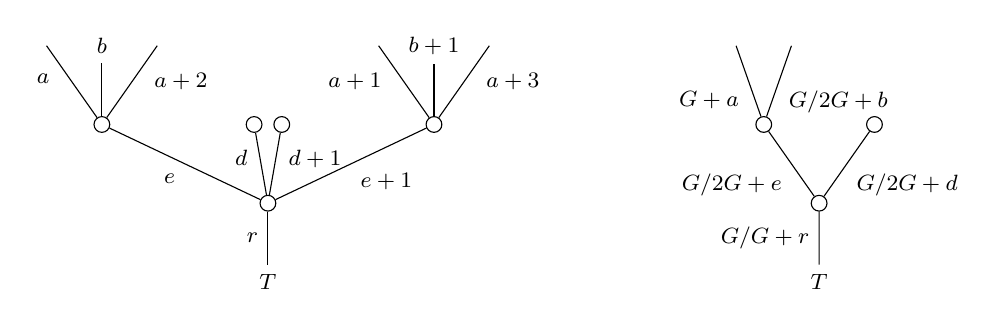
\begin{tikzpicture}[grow= up, auto, level distance = 1cm, every node/.style = {font=\footnotesize}]
              \tikzstyle{level 2}=[sibling distance=4em]
              \tikzstyle{level 3}=[sibling distance=2em]
              \node{$T$}
              child{node [dummy] {}%
                child{node [dummy] {}%
                  child{edge from parent node [swap,near end]{$a+3$}}
                  child{node {$b+1$}}
                  child{edge from parent node [near end] {$a+1$}}
                  edge from parent node [swap]{$e+1$}
                }
                child[sibling distance=1em]{node [dummy] {}
                  edge from parent node [swap,very near end]{$d+1$}
                }
                child[sibling distance=1em]{node [dummy] {}
                  edge from parent node [very near end]{$d$}
                }
                child{node [dummy] {}%
                  child{edge from parent node [swap, near end]{$a+2$}}
                  child{node {$b$}}
                  child{edge from parent node [near end] {$a$}}
                  edge from parent node {$e$}
                }
                edge from parent node {$r$}
              };
              \tikzstyle{level 3}=[sibling distance=2em]
              \node at (7,0){$T$}
              child{node [dummy] {}%
                child{node [dummy] {}
                  edge from parent node [swap]{$G/2G+d$}
                }
                child{node [dummy] {}%
                  child{edge from parent node [swap]{$G/2G + b$}}
                  child{edge from parent node {$G + a$}}
                  edge from parent node {$G/2G+e$}
                }
                edge from parent node {$G/G+r$}
              };
        \end{tikzpicture}
  \end{equation}
  Consider the edge orbit $G e$.
  The following are all proper faces of $T$ which are \textit{not} in the inner horn $\Lambda^{G e}[T]$:
  \begin{equation}
        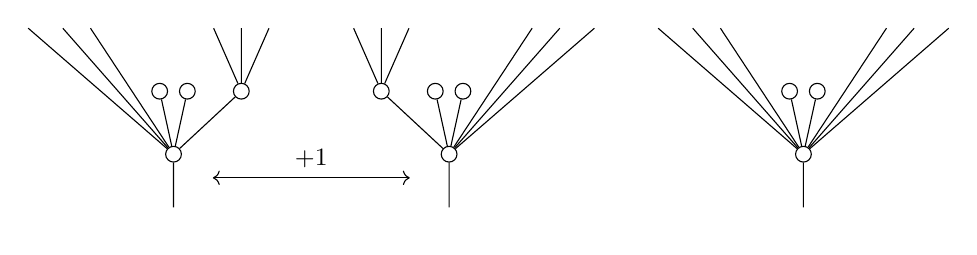
\begin{tikzpicture}
              [grow=up, level distance = .8cm, every node/.style={font=\small}]
              \tikzstyle{level 2}=[sibling distance=1.5em]
              \tikzstyle{level 3}=[sibling distance=1em]
              % -------------- PROPER FACES MISSING FROM \Lambda^{G e}[T] -----------------------------
              \node (Te) at (1,3) {}
              child{node [dummy] {}
                child[sibling distance=.7em]{node [dummy] {}
                  child{}
                  child{}
                  child{}
                }
                child[sibling distance=1em]{edge from parent [draw = none]}
                child[sibling distance=1em]{edge from parent [draw = none]}
                child[sibling distance=1em]{node [dummy] {}}
                child[sibling distance=1em]{node [dummy] {}}
                child[sibling distance=2em,level distance = 1.6cm]{}
                child[sibling distance=1.6em,level distance = 1.6cm]{}
                child[sibling distance=1.5em,level distance = 1.6cm]{}
              };
              \node (Tge) at (4.5,3) {}
              child{node [dummy] {}
                child[level distance = 1.6cm]{}
                child[sibling distance = 1.6em,level distance = 1.6cm]{}
                child[sibling distance = 2em, level distance = 1.6cm]{}
                child[sibling distance = 1em]{node [dummy] {}}
                child[sibling distance = 1em]{node [dummy] {}}
                child[sibling distance=1em]{edge from parent [draw = none]}
                child[sibling distance=1em]{edge from parent [draw = none]}
                child[sibling distance=.7em]{node [dummy] {}
                  child{}
                  child{}
                  child{}
                }
              };
              \draw[<->]
              (Te)+(.5,.5) -- +(3,.5) node [midway, above] {$+1$};
              \node (TGe) at (9,3) {}
              child{node [dummy] {}
                child[level distance = 1.6cm]{}
                child[sibling distance=1.6em,level distance = 1.6cm]{}
                child[sibling distance=2em,level distance = 1.6cm]{}
                child[sibling distance=1em]{node [dummy] {}}
                child[sibling distance=1em]{node [dummy] {}}
                child[sibling distance=2em,level distance = 1.6cm]{}
                child[sibling distance=1.6em,level distance = 1.6cm]{}
                child[sibling distance=1.5em,level distance = 1.6cm]{}
              };
        \end{tikzpicture}
  \end{equation}
  where the tree on the right is a face of both trees in the orbit on the left.
  Similarly, the maximal elements of $\Lambda^{G e}[T]$ are displayed in the top row below,
  while the second row displays the maximal elements of $\Lambda^{G e}_o[T]$;
  we observe that, in this particular case (where each orbit of vertices has at most two elements),
  these are all maximal subfaces of elements in the top row.
  For clarity, we have drawn using dashed lines the inner edges collapsed involving stumps.
    \begin{equation}
        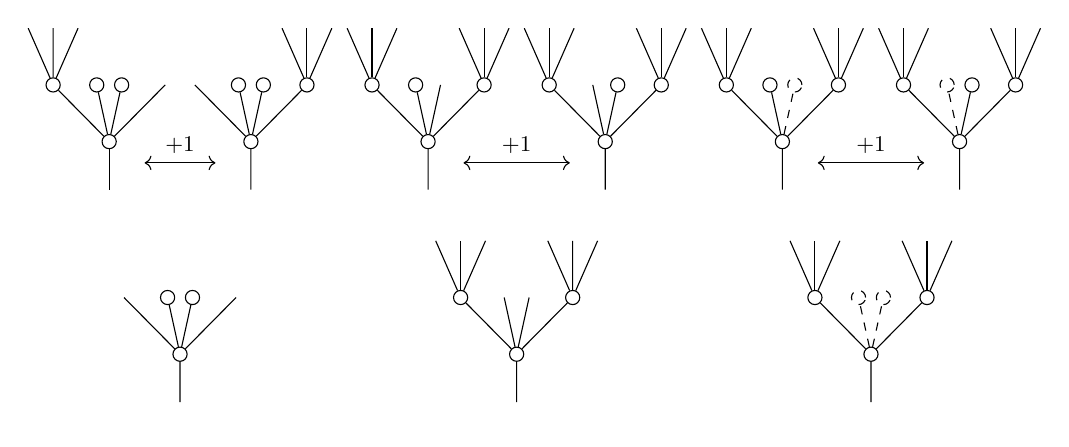
\begin{tikzpicture}
              [grow=up, level distance = .8cm, every node/.style={font=\small, transform shape},
              scale=0.9
              ]
              \tikzstyle{level 2}=[sibling distance=1.5em]
              \tikzstyle{level 3}=[sibling distance=1em]
              % -------------- MAXIMAL FACES OF \Lambda^{G e}[T] --------------------------------------
              \node (TC) {}
              child{node [dummy] {}
                child{}
                child[sibling distance=1em]{node [dummy] {}}
                child[sibling distance=1em]{node [dummy] {}}
                child{node [dummy] {}%
                  child{}
                  child{}
                  child{}
                }
              };
              \node (TgC) at (2,0) {}
              child{node [dummy] {}
                child{node [dummy] {}
                  child{}
                  child{}
                  child{}
                }
                child[sibling distance=1em]{node [dummy] {}}
                child[sibling distance=1em]{node [dummy] {}}
                child{}
              };
              \draw[<->]
              (TC)+(.5,.5) -- +(1.5,.5) node [midway, above] {$+1$};
              \node (TCd) at (4.5,0) {}
              child{node [dummy] {}
                child{node [dummy] {}
                  child{}
                  child{}
                  child{}
                }
                child[sibling distance=1em]{}
                child[sibling distance=1em]{node [dummy] {}}
                child{node [dummy] {}
                  child{}
                  child{}
                  child{}
                }
              };
              \node (TgCd) at (7,0) {}
              child{node [dummy] {}
                child{node [dummy] {}
                  child{}
                  child{}
                  child{}
                }
                child[sibling distance=1em]{node [dummy] {}}
                child[sibling distance=1em]{}
                child{node [dummy] {}
                  child{}
                  child{}
                  child{}
                }
              };
              \draw[<->]
              (TCd)+(.5,.5) -- +(2,.5) node [midway, above] {$+1$};
              \node (Td) at (9.5,0) {}
              child{node [dummy] {}
                child{node [dummy] {}
                  child{}
                  child{}
                  child{}
                }
                child[sibling distance=1em]{node [dummy, dashed] {}
                  edge from parent [dashed]
                }
                child[sibling distance=1em]{node [dummy] {}}
                child{node [dummy] {}
                  child{}
                  child{}
                  child{}
                }
              };
              \node (Tgd) at (12,0) {}
              child{node [dummy] {}
                child{node [dummy] {}
                  child{}
                  child{}
                  child{}
                }
                child[sibling distance=1em]{node [dummy] {}}
                child[sibling distance=1em]{node [dummy, dashed] {}
                  edge from parent [dashed]
                }
                child{node [dummy] {}
                  child{}
                  child{}
                  child{}
                }
              };
              \draw[<->]
              (Td)+(.5,.5) -- +(2,.5) node [midway, above] {$+1$};
              % --------- Maximal Faces in $\Lambda^{G e}_o[T]$ ---------------------------------------%%%%%
              \node (TGC) at (1, -3) {}
              child{node [dummy] {}
                child{}
                child[sibling distance=1em]{node [dummy] {}}
                child[sibling distance=1em]{node [dummy] {}}
                child{}
              };
              \node (TGCd) at (5.75,-3) {}
              child{node [dummy] {}
                child{node [dummy] {}
                  child{}
                  child{}
                  child{}
                }
                child[sibling distance=1em]{}
                child[sibling distance=1em]{}
                child{node [dummy] {}
                  child{}
                  child{}
                  child{}
                }
              };
              % \node (TB) at (7.5,-3) {}
              % child{node [dummy] {}
              %   child{}
              %   child{}
              %   child{}
              %   edge from parent node [left] {$e$}
              % };
              % \node (TgB) at (9,-3) {}
              % child{node [dummy] {}
              %   child{}
              %   child{}
              %   child{}
              %   edge from parent node [right] {$e+1$}
              % };
              % \draw[<->]
              % (TB)+(.3,.5) -- +(1.2,.5) node [midway,above] {$+1$};
              \node (TGd) at (10.75,-3) {}
              child{node [dummy] {}
                child{node [dummy] {}
                  child{}
                  child{}
                  child{}
                }
                child[sibling distance=1em]{node [dummy, dashed] {}
                  edge from parent [dashed]
                }
                child[sibling distance=1em]{node [dummy, dashed] {}
                  edge from parent [dashed]
                }
                child{node [dummy] {}
                  child{}
                  child{}
                  child{}
                }
              };
        \end{tikzpicture}
  \end{equation}
  However, these orbital faces are certainly \textit{not} the only subfaces of the top row above.
  In particular, the following is a minimal face in $\Lambda^{G e}[T]$ not in the orbital horn $\Lambda^{G e}_o[T]$.
  \begin{equation}
        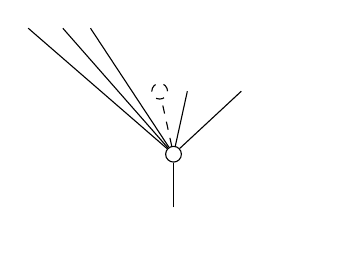
\begin{tikzpicture}
              [grow=up, level distance=.8cm, every node/.style={font=\small}]
              \tikzstyle{level 2}=[sibling distance=2em]
              \tikzstyle{level 3}=[sibling distance=1em]
              \node{}
              child{node [dummy] {}
                child[sibling distance=.7em]{}
                child{edge from parent [draw = none]}
                child{edge from parent [draw = none]}
                child[sibling distance=1em]{}
                child[sibling distance=1em]{node [dummy, dashed] {}
                  edge from parent [dashed]
                }                
                child[sibling distance=2em,level distance = 1.6cm]{}
                child[sibling distance=1.6em,level distance = 1.6cm]{}
                child[sibling distance=1.5em,level distance = 1.6cm]{}
              };
        \end{tikzpicture}
  \end{equation}
\end{example}














\subsection{Proof of \cref{HYPER PROP}}


{\color{red} need to think about hypersaturation for non-monomorphisms}

Recall that a class of maps is called \textit{saturated}
if it is closed under pushouts, transfinite composition and retracts.
Moreover, following the discussion preceding \cite[Prop. 3.6.8]{HHM16}, we will call a class of maps of $\mathsf{dSet}^G$ \textit{hypersaturated} if it is further closed under the following cancellation property: if in
\[
A \xrightarrow{f} B \xrightarrow{g} C
\]
both $f$ and $gf$ are in the class, then so is $g$.

\begin{notation}
      Given a class of morphisms $\mathcal{C}$ in $\mathcal V$, let
      $W(\mathcal C)$ and $\hat{W}(\mathcal C)$ denote
      the saturation and hypersaturation of $\mathcal C$.
      \todo[inline]{change $W$ notation}
\end{notation}

\begin{remark}
      If $L$ is a left adjoint, then $L(\hat{W}(\mathcal C)) \subseteq \hat{W}(L(\mathcal C))$.
      In particular, this applies to the ``free $G$-object'' functor $G \cdot (-)$.
\end{remark}

The following lemma identifies some of the utility of hypersaturations.
\begin{notation}
      Given a class of maps $\mathcal C$ in $\mathcal V$, let $\mathcal C^\boxslash$ (respectively $\mathcal C^{\boxslash !}$)
      denote the class of maps with the
      \textit{(strict) right lifting property} (abreviated (S)RLP) against $\mathcal C$.
\end{notation}
\begin{lemma}
      \label{HYPER_LP_THM}
      Let $\mathcal C$ be a class of maps in $\mathcal V$. Then
      $W(\mathcal C) = {}^\boxslash(\mathcal C^{\boxslash})$,
      $\mathcal C^{\boxslash}= W(\mathcal C)^{\boxslash}$
      and
      $\mathcal C^{\boxslash !} = \hat{W}(\mathcal C)^{\boxslash !}$.
\end{lemma}
\begin{proof}
      It is a straightforward exercise to show that
      if $X \to Y$ has the (S)RLP with respect to a map $A \to B$ (resp. maps $A_\alpha \to A_{\alpha +1}$), then
      $X \to Y$ has the (S)RLP with respect to any pushout or retract of $A \to B$ (resp. the transfinite composite).
      \begin{itemize}
      \item For the pushout, the map $C \to X$ always provides one component of the new lift,
            while $B \to D \to X$ is always a lift over $A \to B$; hence strictness implies strictness.
      \item For the retract, again we have that $B \to D \to X$ is a lift over $A \to B$,
            and hence strictness implies this composite is uniquely determined;
            composing with the section map yields that $D \to X$ is then also uniquely determined.
      \item Both the definition of the lift for the composite and its uniqueness are immediate.
      \end{itemize}
      Now, suppose $X \to Y$ has the SRLP against $A \to B$ and the composite $A \to B \to C$.
      Consider the diagrams below.
      \begin{equation}
            \begin{tikzcd}
                  A \arrow[r] \arrow[d]
                  &
                  X \arrow[d, equal]
                  &&
                  A \arrow[r] \arrow[d]
                  &
                  B \arrow[d] \arrow[r]
                  &
                  X \arrow[d]
                  \\
                  B \arrow[r] \arrow[d]
                  &
                  X \arrow[d]
                  &&
                  B \arrow[r] \arrow[d] \arrow[urr, crossing over, near start, dashed, "\exists ! G"]
                  &
                  X \arrow[r] \arrow[d]
                  &
                  Y \arrow[d, equal]
                  \\
                  C \arrow[r] \arrow[uur, dashed, crossing over, near end, "\exists ! H"]
                  &
                  Y
                  &&
                  C \arrow[r] \arrow[uurr, bend right, crossing over, dashed, "H"']
                  &
                  Y \arrow[r, equal]
                  &
                  Y
            \end{tikzcd}
      \end{equation}
      By assumption, there exist unique lifts $H$ and $G$ as denoted by the dashed arrows.
      It is immediate that both $B \to X$ and $B \to C \xrightarrow{H} X$ are candidates for lift $G$,
      and hence by strictness all three are equal.
      Thus $H$ is also a lift of the bottom-left square.
      Since any lift of the bottom square is also a lift of the rectangle,
      strictness for $A \to B$ implies strictness for $B \to C$.
      \todo[inline]{check what is needed for the first fact, and prove it}
\end{proof}


{\color{blue}
  \todo[inline]{change/combine with ``CHAR PLAYGROUND SECTION''}
\begin{definition}
      Given $T \simeq G \cdot_H T_0$,
      let $U_0 \subseteq T_0$ be a (non-equivariant) subtree, and
      let $K = \mathrm{Stab}_H(U_0)$.
      Suppose we have another subdendroidal set $X \subseteq \Omega[T]$
      which contains all proper outer faces of $U_0$, and
      an inner edge edge $e \in U_0$.
      We say that $K e \subseteq U_0$ is a \textit{characteristic edge orbit} of
      $X \subseteq \Omega[T] \leftarrow \Omega[G \cdot_K U_0]$
      if we have, for any $R_0 \in \mathscr{F}_{\mathrm{Inn}}(U_0)$ containing $e$ as an inner edge,
      \begin{equation}
            R_0 \in \mathscr{F}_{\mathrm{Inn}}(U_0) \cap X
            \mbox{ if and only if }
            R_0 / \bar K e \in \mathscr{F}_{\mathrm{Inn}}(U_0) \cap X,
      \end{equation}
      where $\bar K = \mathrm{Stab}_{K}(R_0)$. 
\end{definition}

\begin{proposition}
      \label{CHAR_HORN_THM}
      Given $T$, $T_0$, $H$, $U_0$, $K$, and $X$ as above.
      If $K e$ is a characteristic edge orbit of $X \subseteq \Omega[T] \leftarrow \Omega[G \cdot_K U_0]$
      then $X \to X \cup \mathsf{im}\left(\Omega[G \cdot_K U_0] \right)$ is inner $G$-anodyne.
\end{proposition}
\begin{proof}
      If $\mathsf{im}(\Omega[G \cdot_K U_0]) = \bigcup_G \Omega[g U_0]$ is already contained in $X$, we are done.
      Assuming otherwise, it suffices to show that for all
      $C \subseteq C'$ $K$-closed convex subsets of $\mathscr{F}_{\mathrm{Inn}}^{K e}(U_0) \setminus X$, the map
      $X_C \to X_{C'}$ is inner $G$-anodyne, where we define
      \begin{equation}
            X_C := X \cup \mathop{\bigcup}\limits_{C/K} \mathsf{im}\left(\Omega[G \cdot_L U_0 \setminus E] \right)
            = X \cup \left( G \cdot_K \mathop{\bigcup}\limits_{C/K} \Omega[U_0 \setminus E] \right),
      \end{equation}
      with the unions taking place in $\Omega[T]$.
      Indeed, once $C = \mathscr{F}_{\mathrm{Inn}}^{K e}(U_0) \setminus X$, we have the pushout
      \begin{equation}
            \begin{tikzcd}
                  G \cdot_K \left( \Lambda^{K e}[U_0] \right) \arrow[d, hookrightarrow] \arrow[r]
                  &
                  X_C \arrow[d]
                  \\
                  G \cdot_K \Omega[U_0] \simeq \Omega[G \cdot_K U_0] \arrow[r]
                  &
                  X \cup \mathsf{im}\left(\Omega[G \cdot_K U_0]\right).
            \end{tikzcd}
      \end{equation}
      Moreover, it suffices to consider $C' = C \cup G\cdot_K(U_0 \setminus D)$ for a set of inner edges $D$,
      without loss of generality $e \not\in D$ and $U_0 \setminus D$ is not in the domain.
      Let $\bar K = \mathrm{Stab}_H(D)$.

      We first claim that (the image of) $\Lambda^{K e}[U_0 \setminus D]$ is in the domain.
      If $S_0$ is an outer face of $U_0 \setminus D$, then
      $S_0$ factors through an outer face of $U_0$, and so $S_0$ is in $X$.
      Further, if $S_0 = U_0 \setminus (D \cup E)$ with $E \cap K e = \varnothing$,
      then concavity implies that $S_0$ is in the domain, as required.

      Second, we claim that no face $S_0 = U_0 \setminus D \cup \bar e$, with $\bar e \subseteq K e$, is in the domain.
      Suppose $U_0 \setminus D \cup \bar e$ is contained in some $U_0 \setminus E$ already attached.
      Then, since $E \cap K e = \varnothing$ we have $U_0 \setminus D \subseteq U_0 \setminus E$, so
      $U_0 \setminus D$ is also in the domain, a contradiction.
      Further, if $U_0 \setminus D \cup \bar e$ is in $X$, then so is $U_0 \setminus D \cup K e$, and hence
      so is $U_0 \setminus D$ (by definition of characteristic edge orbit), also a contradiction.

      Now, all faces $U_0 \setminus D \cup \bar e$ with $\varnothing \subseteq \bar e \subseteq K e$ have stabilizer $\bar K$
      (else $D \cap K e \neq \varnothing$).
      Thus $X_C \to X_{C'}$ is the pushout of
      \begin{equation}
            \label{CHAR_HORN_EQ}
            G \cdot_{\bar K} \left( \Lambda^{\bar K e}[U_0 \setminus D] \to \Omega[U_0 \setminus D] \right),
      \end{equation}
      and hence is anodyne, as required.
\end{proof}



% \begin{proposition}
%       \label{ORB_HORN_THM}
%       $\Lambda_o^{Ge}[T] \to \Omega[T]$ is inner $G$-anodyne, and hence
%       the (hyper)saturated class of the orbital horn inclusions is contained in
%       the (hyper)saturated class of the horn inclusions.
% \end{proposition}
% \begin{proof}
%       Let $\mathrm{Out}^{-o}(T)$ be the poset of outer faces $U_0$ of $T$ which are not in $\Lambda_0^{Ge}[T]$.
%       It suffices to show that for any $G$-convex subsets $B \subseteq B'$ of $\mathrm{Out}^{-o}(T)$, the map
%       \begin{equation}
%             \left(\Lambda^{G e}_{o}[T]\right)_B
%             := \Lambda_o^{Ge}[T] \cup \mathop{\bigcup}\limits_{B/G}\mathsf{im}\left(\Omega[G \cdot_K U_0]\right)
%             \to
%             \Lambda_o^{Ge}[T] \cup \mathop{\bigcup}\limits_{B'/G}\mathsf{im}\left(\Omega[G \cdot_K U_0]\right)
%             =: (\Lambda^{G e}_o[T])_{B'}
%       \end{equation}
%       is inner $G$-anodyne.
%       Again, suffices to show when $B' = B \cup G \cdot_K \set{U_0}$, where $K = \mathrm{Stab}_G(U_0)$, and
%       without loss of generality $e \in U_0$.
%       For the final reduction, \cref{CHAR_HORN_THM} implies it suffices to show
%       $K e$ is a characteristic edge orbit for
%       $(\Lambda^{G e}_o[T])_B \subseteq \Omega[T] \leftarrow \Omega[G \cdot_K U_0]$.
%       To that end, let $U_0 \setminus D$ be an inner face with stabilizer $\bar K$.
      
%       For $B = \varnothing$, we suppose $U_0 \setminus \bar K e \in \Lambda_o^{G e}[T]$. This implies that
%       \begin{equation}
%             K_r := \mathrm{Stab}_H(r_U) \leq \mathrm{Stab}_H(U_0 \setminus D \cup \bar K e) \leq \mathrm{Stab}_H(U_0) \leq Kr,
%       \end{equation}
%       so the outer face $U_0$ is $K_r$-closed and not in $\Lambda_0^{Ge}[T]$, and hence we conclude that $U_0$ must be $T_0$.
%       However, if $\Lambda^{Ge}_0[T] \neq \Lambda^{Ge}[T]$, $T_0$ is not a minimal outer face not in $\Lambda_0^{Ge}[T]$.
%       Thus, in these cases, $K e$ is a characteristic edge orbit vacuously.
%       If in fact $\Lambda_o^{Ge}[T] = \Lambda^{Ge}[T]$, then $T \simeq G \cdot T_0$, so $H = \bar K = K_r = \set{e}$.
%       Now, since $U_0 \setminus D \cup e \in \Lambda_0^{Ge}[T]$,
%       $D \setminus e \neq \varnothing$, so
%       $U_0 \setminus D \in \Lambda_0^{Ge}[T]$.
      
%       For general $B$, we know the domain contains all outer faces of $U_0$ by convexity.
%       Now, let $U_0 \setminus D$ be an inner face, with stabilizer $\bar K$.
%       Then $U_0 \setminus D \cup \bar K e$ is in the domain if either
%       $U_0 \setminus D \cup \bar K e$ is contained in some $\Omega[G \cdot_L R_0]$, or
%       $U_0 \setminus D \cup \bar K e \in \Lambda_o^{Ge}[T]$.
%       But then $U_0$ is contained in $R_0$ since both are outer faces, or again we apply the previous lemma.
%       Both lead to contradictions, and thus the result follows.
% \end{proof}

 }%%%%%%%%%%%-------------- COLOR BLUE --------------------------------------------------------------------




The reverse inclusion is only true on the level of hypersaturations.
\begin{definition}
      Let $\hat{W}_o$ be the hypersaturation of the orbital horn inclusions.
\end{definition}

\begin{proposition}
      \label{HORN_ORB_THM}
      For any $T \in \Omega_G$, the map
      $\Lambda^{G e}[T] \to \Omega[T]$
      is in $\hat{W}_o$.
\end{proposition}
\begin{proof}
      We go by induction on $|G| \times |\mathscr{F}_{\mathrm{Inn}}(T)|$ \todo{replace $Inn(T)$ with $Inn_G(T)$? $E(T)$? $V(T)$? $V_G(T)$?}
      When $G = \set{e}$, the orbital horns are regular inner horns, and so the result holds.

      Now, the proof of \cref{CHAREDGE LEM} says that,
      for any proper face $U_0 \into T$,
      if $E$ is a characteristic edge set for $U_0$ with respect to $X$, then
      \begin{equation}
            \label{CHAR_ATTACH_EQ}
            X \to X \cup \mathop{\bigcup}\limits_G \Omega[g U_0]
      \end{equation}
      is cellular on inner horn inclusions of for inner faces of $U_0$,
      and thus such maps \eqref{CHAR_ATTACH_EQ} are in $\hat{W}_o$ by induction
      (since either $|\mathrm{Stab}_G(U_0)| < |G|$ or $U_0$ is strictly contained in a component of $T$).

      We now claim that
      \begin{equation}
            \Lambda^{G e}_o[T] \to \Lambda_o^{G e}[T] \cup \partial^{out}\Omega[T] =:A
      \end{equation}
      is in $\hat{W}_o$.
      Indeed, letting $\mathsf{Out}^{-o}(T)$ denote the poset of proper outer faces $U_0$ of $T$
      which are not in $\Lambda_o^{G e}[T]$,
      it suffices to show that for any $G$-convex $B \subseteq B' \subseteq \mathsf{Out}^{-o}[T]$,
      the map
      \begin{equation}
            (\Lambda^{G e}_o[T])_B := \Lambda^{G e}_o[T] \cup  \mathop{\bigcup}\limits_{B}\Omega[U_0]
            \to
            \Lambda^{G e}_o[T] \cup  \mathop{\bigcup}\limits_{B'}\Omega[U_0]
      \end{equation}
      is built from a characteristic edge construction.
      We may assume $B' = B \cup G\set{U_0}$, and then apply \cref{CHAREDGE LEM} with
      $X = (\Lambda^{G e}_o[T])_B$, $\set{U_i} = \set{g U_0}$, and $\Ksi = G e$. 
      (Ch 0) and (Ch 3') are immediate, and (Ch 1) follows by convexity.
      (Ch 2) follows as in the proof of \cref{ORB_HORN_THM}.

      % {\color{blue}     
      %   Thus, the proof of \cref{ORB_HORN_THM} implies, in particular, that
      %   \begin{equation}
      %         \Lambda^{G e}_o[T] \to \Lambda^{G e}_o[T] \cup \partial^{out}(T) =: A
      %   \end{equation}
      %   is in $\hat{W}_o$.
      % }%%% ------------ COLOR BLUE -------------------------------------------

      Lastly, it then suffices to show that
      $\Ksi = H e$ is a characteristic edge set for $\set{U_i} = \set{T_0}$ with respect to $X = A$,
      where $e \in T_0$ and $T \simeq G \cdot_H T_0$ is a decomposition for $T$.
      (Ch 0) and (Ch 3') are immediate, while (Ch 1) follows since $\partial^{out}\Omega[T] \subseteq A$.
      Finally, since any inner face $V_0$ of $T_0$ is not contained in any outer face,
      (Ch 2) follows as above:
      if $V_0 - He$ is contained in the orbital horn, then so is $V_0$ by \cref{GINNER REM}.
    
      % It then suffices to show that, for any $G$-convex subposets $B \subseteq B' \subseteq \mathscr{F}_{\mathrm{Inn}}^{G e,-o}(T)$,
      % \begin{equation}
      %       \label{ORB_HORN_ATTACH_EQ}
      %       A_B := A \cup \mathop{\bigcup}\limits_{B/G}\mathsf{im}\left(\Omega[G \cdot_{K} U_0]\right)
      %       \to
      %       A \cup \mathop{\bigcup}\limits_{B'/G}\mathsf{im}\left(\Omega[G \cdot_{K} U_0]\right) =: A_B'
      % \end{equation}
      % is in $\hat{W}_o$,
      % where $\mathscr{F}_{\mathrm{Inn}}^{G e,-o}(T)$ is the poset of inner faces of $T$ which contain $H e$ and are not in $\Lambda^{G e}_o[T]$.
      % Indeed, for $B = \mathscr{F}_{\mathrm{Inn}}^{G e,-o}(T)$, $A_B = \Lambda^{G e}[T]$,
      % so the result follows from the cancelation property in the definition of hypersaturation.

      % We may assume that $B' = B \cup (G\cdot_K \set{U_0})$, for $U_0 = T_0 \setminus D$.
      % % and let's call the domain of \eqref{ORB_HORN_ATTACH_EQ} $A_B$.
      % Then, it suffices to show that $K e$ is a characteristic edge orbit for
      % $A_B \subseteq \Omega[T] \leftarrow \Omega[G \cdot_K U_0]$.
      % Since $A_B$ contains all outer faces of $T$ (and hence all outer faces of $U_0$),
      % let $R_0 = T_0 \setminus D \cup E$ be an inner face of $U_0$ with isotropy $\bar K$, and suppose
      % $R_0 \setminus \bar K e$ is in $A_B$.
      % We see $R_0 \setminus \bar K e \in \Lambda^{G e}_o[T]$ iff $D \cup E$ contains a full $H$-orbit $H t$ of edges, in which case
      % \begin{equation}
      %       R_0 \setminus \bar K e = T_0 \setminus D \cup E \cup K e
      %       \into
      %       T_0 \setminus H t \in \Lambda^{G e}_o[T].
      % \end{equation}
      % But then we also have $R_0 = T_0 \setminus D \cup E \into T_0 \setminus H t$, as required.
      % Moreover, no inner face factors through an outer face of $T$.
      % Finally, if $R_0 \setminus \bar K e$ is in some $S_0 = T_0 \setminus D'$ already attached, then
      % $D \cup E \cup \bar K e \supseteq D'$;
      % but since $D' \cap K e = \varnothing$, this implies
      % $D \cup E \supseteq D'$, and hence $R_0$ also factors through $S_0$, as required.
      % Thus $K e$ is a characteristic edge orbit, and the result is proven.
\end{proof}



We will now compare Segal core inclusions with the inner horn inclusions.

\begin{proposition}
      \label{SC_IN_GHORN_THM}
      For all $T \in \Omega_G$, $Sc[T] \to \Omega[T]$ is inner $G$-anodyne.
\end{proposition}
\begin{proof}
      Let $\mathsf{Out}^{>1}(T)$ denote the subposet $\mathsf{Out}(T) \setminus \mathscr{F}_{\mathrm{SC}}(T)$.
      It suffices to show that for all $G$-convex $B \subseteq B' \subseteq \mathsf{Out}^{>1}(T)$, the map
      \begin{equation}
            % (Sc[T])_B :=
            % Sc[T] \cup \mathop{\bigcup}\limits_{B/G}\mathsf{im}(\Omega[G \cdot_K U_0])
            Sc[T] \cup \mathop{\bigcup}\limits_{B}\Omega[U_0]
            \to
            Sc[T] \cup \mathop{\bigcup}\limits_{B'}\Omega[U_0]
            % Sc[T] \cup \mathop{\bigcup}\limits_{B'/G}\mathsf{im}(\Omega[G \cdot_K U_0])
      \end{equation}
      is inner $G$-anodyne. In particular, we may assume $B' = B \cup G \cdot_K \set{U_0}$.
      Then the above map is the pushout over
      \begin{equation}
                  G\cdot_K \left(\partial^{out}\Omega[U_0] \to \Omega[U_0] \right),
      \end{equation}
      which by \cref{GEN_GHORN_THM} is inner $G$-anodyne, and hence the result follows.
\end{proof}
\begin{proof}
      Fix some decomposition $T \simeq G \cdot_H T_0$, and let $I_0$ denote the set of inner edges of $T_0$.
      Then it is immediate that $I_0$ is an characteristic inner edge set for $T_0$ with respect to $Sc[T]$,
      and the result then follows from \cref{CHAREDGE LEM}.
\end{proof}
\begin{proposition}
      \label{SC_IN_OHORN_THM}
      For all $T \in \Omega_G$, $Sc[T] \to \Omega[T]$ is in $W_o$. 
\end{proposition}
\begin{proof}
      Define $\mathscr{F}'_{o}(T)$ denote the poset of orbital non-vertex-inclusion outer faces
      $\mathscr{F}_{o}^{G e}(T) \setminus \mathscr{F}_{SC}(T)$.
      It suffices to show that for all $G$-convex $B \subseteq B' \subseteq \mathscr{F}'_o(T)$, the map
      \begin{equation}
            % Sc[T] \cup \mathop{\bigcup}\limits_{B/G}\mathsf{im}\left(\Omega[G \cdot_K U_0]\right)
            Sc[T] \cup \mathop{\bigcup}\limits_{B}\Omega[U_0]
            \to
            Sc[T] \cup \mathop{\bigcup}\limits_{B'}\Omega[U_0]
            % \mathop{\bigcup}\limits_{B'/G}\mathsf{im}\left(\Omega[G \cdot_K U_0]\right)
      \end{equation}
      is in $W_o$; in particular, we may assume $B' = B \cup G \cdot_K U_0$.

      Now, since $B$ is convex, every orbital face of $U_0$ is in the domain.
      Continuing, any face in $\Omega[G \cdot_K U_0] \cap Sc[T]$ is in $Sc[G \cdot_K U_0] \subseteq \partial^{out}_o[G \cdot_K U_0]$.
      Moreover, any face $R_0$ in $\Omega[G \cdot_K U_0] \cap \Omega[G \cdot_L V_0]$ for $V_0$, another orbital face,
      is a face of their intersection (where we may assume $R_0$ injects into both $U_0$ and $V_0$),
      which is also orbital.
      Thus, the above map is the pushout over
      \begin{equation}
            \partial^{out}_o[G \cdot_K U_0] \to \Omega[G \cdot_K U_0].
      \end{equation}
\end{proof}
The above combined with \cref{ORB_HORN_THM} immediately implies the following.
\begin{corollary}
      Segal core inclusions are inner $G$-anodyne.
\end{corollary}


\begin{definition}
      Let $\hat{W}_{SC} = \hat{W}(SCI_G)$ denote the hypersaturation of the Segal core inclusions.
\end{definition}

\begin{lemma}
      \label{GHORN_IN_SC_THM}
      The inner $G$-horn inclusions are contained in $\hat{W}_{SC}$.
\end{lemma}
\begin{proof}
      It suffices to show that $\Lambda^{G e}[T] \to \Omega[T]$ is in $\hat{W}_{SC}$
      for any $T\in \Omega_G$ and inner edge $e$ of $T$.

      Suppose we have a decomposition $T \simeq G \cdot_H T_0$, where $H = \mathrm{Stab}(T_0)$.
      We go by induction on $|H| \times |V_H(T_0)|$.

      If $H = e$, then, since $G \cdot SCI \subseteq SCI_G$,
      and by \cite[2.5]{CM13a} we know $IHI \subseteq \hat{W}(SCI)$, we conclude that
      \begin{equation}
            G \cdot IHI \subseteq G \cdot (\hat{W}(SCI)) \subseteq \hat{W}(G \cdot SCI) \subseteq \hat{W}(SCI_G) = \hat{W}_{SC}.
      \end{equation}
      
      If $H \neq e$, and $V_H(T_0) = 2$, then there is only one inner edge orbit, so
      the Segal core is an inner horn.
      Thus, we may assume that $V_H(T_0) > 2$.

      By \cref{GHORN_IN_SC_THM}, we see that
      \begin{equation}
            \label{SC_POUT_EQ}
            Sc[T] \to \partial^{out}\Omega[T]
      \end{equation}
      is cellular on maps of the form
      $\partial^{out}[G \cdot_K U_0] \to \Omega[G \cdot_K U_0]$ for outer faces $U_0$ of $T$,
      which are themsevles inner $G$-anodyne on inner horn inclusions in trees either
      with strictly smaller isotropy (e.g. $K \leq H$) or
      with a strictly smaller number of $G$-vertices.
      Thus, by induction, \eqref{SC_POUT_EQ} is in $\hat{W}_{SC}$. 

      Now consider
      \begin{equation}
            \label{POUT_GHORN_EQ}
            \partial^{out}\Omega[T] \to \Lambda^{G e}[T].
      \end{equation}
      By \cite[Proposition 6.17]{Per17},
      this is built by pushouts over maps of the form
      $\partial^{out}\Omega[G \cdot_K U_0] \to \Omega[G \cdot_K U_0]$ for $U_0 \in \mathscr{F}_{\mathsf{Inn}}^{H e}[T_0]$,
      and so again by induction on $|H| \times |V_H(T_0)|$, these maps are all in $\hat{W}_{SC}$. 
      
      Combining the above, we have that $Sc[T] \to \Lambda^{G e}[T]$ is in $\hat{W}_{SC}$, and hence
      by the closure property of hypersaturations, the inner horn inclusion $\Lambda^{G e}[T] \to \Omega[T]$
      is in $\hat{W}_{SC}$, as desired.
\end{proof}





The following is an equivariant generalization of 
\cite[Props. 2.4 and 2.5]{CM13a},
summarizing the results
(in particular, \cref{ORB_HORN_THM}, \cref{HORN_ORB_THM} \cref{SC_IN_GHORN_THM}, \cref{SC_IN_OHORN_THM}, and \cref{GHORN_IN_SC_THM})
of this subsection.

\begin{proposition}
The following sets of maps generate the same hypersaturated class:
\begin{itemize}
\item the $G$-inner horn inclusions
$\Lambda^{Ge} [T] \to \Omega[T]$ for $T \in \Omega_G$ and $Ge$ an inner edge orbit; 
\item the orbital $G$-inner horn inclusions
$\Lambda^{Ge}_o [T] \to \Omega[T]$ for $T \in \Omega_G$ and $Ge$ an inner edge orbit; 
\item the $G$-segal core inclusions
$Sc [T] \to \Omega[T]$ for $T \in \Omega_G$.
\end{itemize}
Moreover, one also has the following:
\begin{itemize}
	\item[(a)] orbital $G$-inner horn inclusions are in the saturation of $G$-inner horn inclusions;
	\item[(b)] $G$-segal core inclusions are in the saturation of both orbital $G$-inner horn and $G$-inner horn inclusions.
\end{itemize}
\end{proposition}


As a corollary of the above, we can fully characterize the image of the nerve functor $N: \Op^G \to \mathsf{dSet}^G$.

\begin{definition}
      $X \in \mathsf{dSet}^G$ is called a \textit{(strict) inner $G$-Kan complex} if
      $X$ has the strict right lifting property against inner $G$-horn inclusions
      (that is, $(X \to \**) \in (IHI_G)^{\boxslash (!)}$).
      Let $\mathsf{(S)Kan}_G \subseteq \mathsf{dSet}^G$ denote the full subcategory.

      Similarly, let $\mathsf{(S)Kan}$ denote the category of
      (strict) inner Kan complexes in $\mathsf{dSet}$
      (that is, $(X \to \**) \in (IHI)^{\boxslash (!)}$).
      We will denote their image under $\iota_!$ by $(S)Kan^G = G \cdot (S)Kan$.
      \todo[inline]{make sure we say $(\iota_!)\Lambda^E[T_0] = \Lambda^{G E}[G \cdot T_0]$ somewhere}
\end{definition}

\begin{remark}
      If $IHI$ denotes the set of inner horn inclusions in $\mathsf{dSet}$,
      with image $\iota_! IHI = G \cdot IHI$ in $\mathsf{dSet}^G$,
      then it is immediate that $(G \cdot IHI)^{\boxslash} = Kan^G$ and $(G \cdot IHI)^{\boxslash !} = SKan^G$.
\end{remark}

We will in fact show that $(G \cdot IHI)^{\boxslash !} = (IHI_G)^{\boxslash !}$.
First, a lemma.

\begin{lemma}
      Let $GIHI$ denote the class of generalized inner horn inclusions $\Lambda^E[T_0] \to \Omega[T]$. 
      If $X \in (G\ cdot IHI)^{\boxslash !}$, then
      $X \in (G \cdot GIHI)^{\boxslash !}$. 
\end{lemma}
\begin{proof}
      We go by induction on $|V(T_0)| \times |E|$, where the base case is immediate.
      Now, given $e\in E$, the square below is a pushout.
      \begin{equation}
            \begin{tikzcd}
                  \iota_!\Lambda^{E\setminus e}[T_0/e] \arrow[rr] \arrow[d]
                  &&
                  \iota_!\Lambda^E[T_0] \arrow[r, "f"]
                  &
                  X
                  \\
                  \iota_!\Omega[T_0/e] \arrow[rr] \arrow[urrr, dotted, near start, "\exists! F"]
                  &&
                  \iota_!\Lambda^{E\setminus e}[T_0] \arrow[ur, dotted, "\exists! F'"'] \arrow[u, leftarrow, crossing over]
            \end{tikzcd}
      \end{equation}
      Moreover, by induction, any map $f$ induces a unique lift $F$.
      The universal property of the pushout then implies that we have a unique lift $F'$.

      Now, we have the following diagram
      \begin{equation}
            \begin{tikzcd}
                  \iota_!\Lambda^{E}[T_0] \arrow[rr, "f"] \arrow[d, "i"']
                  &&
                  X \arrow[d, equal]
                  \\
                  |[alias = U]| (i_G)_!\Lambda^{E \setminus e}[T_0] \arrow[d, "j"'] \arrow[rr, dotted, near end, "\exists! F'"]
                  &&
                  |[alias=V]| X
                  \\
                  \iota_!\Omega[T_0]
                  \arrow[uurr, dotted, near end, crossing over, "\exists \psi"] \arrow[urr, dotted, "\exists! \phi"']
                  % \arrow[dotted, from=U, to=V, crossing over, "\exists! g"] \\
            \end{tikzcd}
      \end{equation}
      where the dotted arrows are lifts:
      $F'$ is the unique lift of $f$ against $i$,
      $\phi$ is the unique lift of $F'$ against $j$, and
      $\psi$ is some lift of $f$ over $ji$.
      This implies that $\psi j$ is a lift of $f$ over $i$, so by uniquenss $\psi j = F'$, but then
      $\psi$ is a lift of $F'$ over $j$, and hence $\psi = \phi$,
      Thus the lift of $f$ over $j i$ is uniquely determined.
\end{proof}

\begin{proposition}
      \label{SRLP_IHI_THM}
      $(IHI_G)^{\boxslash !} = (G\cdot IHI)^{\boxslash !}$.
      Thus $\mathsf{Kan}_G = \mathsf{Kan}^G$
      % (strict inner $G$-Kan complexes are just $G$-objects in strict inner Kan complexes)
\end{proposition}
\begin{proof}
      Any inner $G$-horn inclusion $i: \Lambda^{G e}[T] \to \Omega[T]$ has a decomposition description as
      \begin{equation}
            j/N: (\iota_! \Lambda^{H e}[T_0])/N \to (\iota_! \Omega[T_0])/N,
      \end{equation}
      where $e \in T_0$, $T \simeq G \cdot_H T_0 \simeq (G \cdot T_0)/N$, $N$ a graph subgroup of $G \times \mathsf{Aut}(T_0)$,
      and $j \in GIHI$.
      Now, for any span
      $\Omega[T] \xleftarrow{j/N} \Lambda^{G e}[T] \xrightarrow{f}$,
      consider the following diagram, where $n \in N$, and the dashed arrows are lifts.
      \begin{equation}
            \begin{tikzcd}
                  \iota_!\Lambda^{H e}[T_0] \arrow[dd, "j"'] \arrow[rr] \arrow[dr, "n"]
                  &&
                  \iota\Lambda^{H.e}[T_0]/N \simeq \Lambda^{G e}[T] \arrow[dd, "j/N = i"] \arrow[r, "f"]
                  &
                  X
                  \\
                  &
                  \iota_!\Lambda^{H.e}[T_0] \arrow[dd] \arrow[ur, twoheadrightarrow]
                  \\
                  \iota_!\Omega[T_0] \arrow[rr, crossing over]
                  \arrow[uurrr, crossing over, bend right=10, very near start, dotted, "\exists! \phi"] \arrow[dr, "n"]
                  &&
                  \iota_!\Omega[T_0]/N \simeq \Omega[T]
                  \\
                  &
                  \iota_!\Omega[T_0] \arrow[ur, twoheadrightarrow] \arrow[uuurr, dotted, out=0, in=-90, "\exists! \phi"']
            \end{tikzcd}
      \end{equation}
      Uniqueness implies that $\phi = n \cdot \phi$ for all $n \in N$, and hence factors through $\Omega[T]$,
      finishing the proof.
\end{proof}

\begin{corollary}
      Fix $X \in \mathsf{dSet}^G$. Then
      $X$ is a strict inner $G$-Kan complex iff $X \simeq N^G(\O)$ for some $\O \in \mathsf{Op}^G$.
\end{corollary}
\begin{proof}
      $N^G(\O)(T)$ is given by maps $\mathsf{Op}^G(\Omega(T), \O)$,
      and since $\Omega(T)$ is a free coloured operad on it's vertices, we may conclude that
      \begin{equation}
            N^G(\O)(T) \simeq \mathsf{Op}^G(\Omega(T), \O) \simeq \mathsf{dSet}^G(Sc[T], N^G\O).
      \end{equation}
      Thus $N^G(\O)$ is in $(SCI_G)^{\boxslash !}$, and hence is in $(IHI_G)^{\boxslash !}$
      by \cref{HYPER_LP_THM,GHORN_IN_SC_THM}.

      Conversely, by \cref{SRLP_IHI_THM} and \cite[Theorem 6.1, Proposition 6.10]{MW09}, we have that
      $X \simeq N_d \circ \tau_d \circ X$
      (where we consider $X$ as a functor $G \to \mathsf{Kan}$).
\end{proof}














\subsection{Weak Equivalences in $\mathsf{dSet}^G$}

Recall that a class of maps is called \textit{saturated}
if it is closed under pushouts, transfinite composition and retracts.
Moreover, following the discussion preceding \cite[Prop. 3.6.8]{HHM16}, we will call a class of maps of $\mathsf{dSet}^G$ \textit{hypersaturated} if it is further closed under the following cancellation property: if in
\[
A \xrightarrow{f} B \xrightarrow{g} C
\]
both $f$ and $gf$ are in the class, then so is $g$.

The following is an equivariant generalization of 
\cite[Props. 2.4 and 2.5]{CM13a}.

\begin{proposition}\label{HYPER PROP}
The following sets of maps generate the same hypersaturated class:
\begin{itemize}
\item the $G$-inner horn inclusions
$\Lambda^{Ge} [T] \to \Omega[T]$ for $T \in \Omega_G$ and $Ge$ an inner edge orbit; 
\item the orbital $G$-inner horn inclusions
$\Lambda^{Ge}_o [T] \to \Omega[T]$ for $T \in \Omega_G$ and $Ge$ an inner edge orbit; 
\item the $G$-segal core inclusions
$Sc [T] \to \Omega[T]$ for $T \in \Omega_G$.
\end{itemize}
Moreover, one also has the following:
\begin{itemize}
	\item[(a)] orbital $G$-inner horn inclusions are in the saturation of $G$-inner horn inclusions;
	\item[(b)] $G$-segal core inclusions are in the saturation of both orbital $G$-inner horn and $G$-inner horn inclusions.
\end{itemize}
\end{proposition}


\begin{remark}
	Setting $G=e$ and slicing over the stick tree $\eta$ in the previous result
	one recovers the well known claim that 
	the hypersaturation of the simplicial inner horns
	$\{\Lambda^i[n] \to \Delta[n] \colon 0< i < n\}$
	coincides with the hypersaturation of the simplicial Segal core inclusions
	$\{Sc[n] \to \Delta[n]\colon n \geq 2\}$.
\end{remark}


\begin{remark}\label{HYPERSATKAN REM}
	We will also make use of a variant of the previous remark for the hypersaturation of \textit{all} simplicial horns.
	Namely, we claim that the hypersaturation of all simplicial horns 
	$\{\Lambda^i[n] \to \Delta[n] \colon 0 \leq i \leq n\}$
	coincides with the hypersaturation of all vertex inclusion maps
	$\{\Delta[0] \to \Delta[n]\}$.
	Indeed, call the latter hypersaturation $S$. 
	An easy argument shows that the Segal core inclusions 
	$\{Sc[n] \to \Delta[n]\}$ are in $S$ and thus so are all inner horn inclusions. On the other hand, the skeletal filtration of the left horns $\Lambda^0[n]$ is built exclusively out of left horn inclusions, and thus since $\Delta[0]=\Lambda^0[1] \to \Delta[1]$ is in $S$ so are all left horn inclusions 
	$\Lambda^0[n] \to \Delta[n]$. The case of right horn inclusions $\Lambda^n[n] \to \Delta[n]$ is dual.
\end{remark}

\begin{notation}
Given subgroups $H_i \leq G$, $0\leq i \leq k$ such that
$H_0 \geq H_i$, $1 \leq i \leq k$ we write
$C_{\amalg_i H_0/H_i}$ for the $G$-corolla encoding the 
$H_0$-set $H_0/H_1 \amalg \cdots \amalg H_0/H_k$.
\end{notation}


The following is the equivariant generalization of 
\cite[Thm. 3.5]{CM13a}.

\begin{proposition}\label{TFAE PROP}
Let $X \to Y$ be a map between $G$-$\infty$-operads. The following are equivalent:
\begin{enumerate}
	\item[(a)] for all $G$-corollas $C_A$ and $H\leq G$ the maps
\[k(\Omega[C_A],X) \to k(\Omega[C_A],Y), \qquad
k(\Omega[G/H \cdot \eta],X) \to k(\Omega[G/H \cdot \eta],Y)
\]
are weak equivalences in $\mathsf{sSet}$;
	\item[(b)] for all $G$-trees $T$ the maps 
	\[k(\Omega[T],X) \to k(\Omega[T],Y) \]
are weak equivalences in $\mathsf{sSet}$;
	\item[(c)] for all normal $G$-dendroidal sets $A$, the maps
	\[k(A,X) \to k(A,Y) \]
are weak equivalences in $\mathsf{sSet}$;
	\item[(d)] $f \colon X \to Y$ is a weak equivalence in 
	$\mathsf{dSet}^G$.
\end{enumerate}
\end{proposition}


\begin{definition}\label{PROF DEF}
	Let $X$ be a $G$-$\infty$-operad.
	A \textit{$G$-profile} on $X$ is a map
\[
	\partial \Omega[C] \to X
\]
	for some $G$-corolla $C \in \Sigma_G$.

More explicitly, a $G$-profile consists of:
\begin{itemize}
	\item subgroups $H_i \leq G$, $0\leq i \leq k$ such that
	$H_0 \geq H_i$ for $1 \leq i \leq k$;
	\item objects $x_i \in X(\eta)^{H_i}$ for $0 \leq i \leq k$.
\end{itemize}
To simplify notation, we will prefer to denote a $G$-profile as 
$(x_1,\cdots,x_k;x_0)$, and refer to it as a 
\textit{$C$-profile}.
\end{definition}


\begin{definition}\label{MAPSPACE DEF}
Given a $G$-$\infty$-operad and a $C$-profile 
$(x_1,\cdots,x_k;x_0)$ we define the space of maps
$X(x_1,\cdots,x_k;x_0)$ to be given by the pullback
\[
\begin{tikzcd}
	X(x_1,\cdots,x_k;x_0) \ar{r} \ar{d}&
	Hom(\Omega[C],X) \ar{d}
\\
	G \cdot \eta \ar{r}[swap]{(x_1,\cdots,x_k;x_0)} &
	\prod_{0\leq i \leq k} X^{H_i}
\end{tikzcd}
\]
Noting that there are equivalences of categories (the first of which is an isomorphism)
\[(\mathsf{dSet}_G) / G\cdot \eta \simeq 
\mathsf{sSet}^{B_G} \simeq \mathsf{sSet},\]
 one sees that 
$X(x_1,\cdots,x_k;x_0)$ 
can indeed be regarded as a simplicial set (in fact, this is a Kan complex).
\end{definition}


\begin{definition}
Let $f \colon X \to Y$ be a map of $G$-$\infty$-operads.

The map $f$ is called \textit{fully faithful} if, for each $C$-profile $(x_1,\cdots, x_k ; x_0)$ one has that
\[
X(x_1,\cdots,x_k;x_0) \to Y\left(f(x_1),\cdots,f(x_k);f(x_0)\right)
\]
is weak equivalence in $\mathsf{sSet}$.

The map $f$ is called \textit{essentially surjective} if for each subgroup $H \leq G$ the map of categories
$\tau(\iota^{\**}(X^H)) \to \tau(\iota^{\**}(Y^H))$
are essentially surjective.
\end{definition}

The following is the equivariant generalization of 
\cite[Thm. 3.11 and Remark 3.12]{CM13a}.


\begin{theorem}\label{COMSQ THM}
A map $f \colon X \to Y$ of $G$-$\infty$-operads is fully faithful iff for all $G$-corollas $C \in \Sigma_G$ the commutative squares
of Kan complexes
\begin{equation}\label{COMSQ EQ}
\begin{tikzcd}
	k(\Omega[C],X) \ar{r} \ar{d}[swap]{p}&
	k(\Omega[C],Y) \ar{d}{q}
\\
	k(\partial \Omega[C],X) \ar{r}[swap]{f_{\**}} &
	k(\partial \Omega[C],Y)
\end{tikzcd}
\end{equation}
are homotopy pullback squares.

Hence, $f$ is a weak equivalence in $\mathsf{dSet}^G$ iff $f$ is both fully faithful and essentially surjective. 
\end{theorem}

\begin{proof}
Noting that the $0$-simplices of $k(\partial \Omega[C],X)$
are precisely the $C$-profiles $(x_1,\cdots,x_k,x_0)$,
fully faithfulness can be reinterpreted as saying that all fiber maps
$p^{-1}(x_1,\cdots,x_k,x_0) \to 
q^{-1}(f(x_1),\cdots,f(x_k),f(x_0))$
are weak equivalences. But since $p,q$ are Kan fibrations, this is equivalent to the condition that \eqref{COMSQ EQ}
is a homotopy pullback (see \cite[Lemma 3.9]{CM13a}), and the first half follows.

For the second half, note first that the bottom map in 
\eqref{COMSQ EQ} can be rewritten as
\[
	\prod_{0\leq i \leq k} k \left(G/H_i \cdot \eta, X \right) \to 
	\prod_{0\leq i \leq k} k \left(G/H_i \cdot \eta, Y \right).
\]

Assume first that $f$ is a weak equivalence. Proposition \ref{TFAE PROP} then implies that the horizontal maps in \eqref{COMSQ EQ}
are weak equivalences, so that the square is a pull back square, and thus $f$ is fully faithful. 
That $f$ is essentially surjective follows from the identity
$k \left(G/H \cdot \eta, X \right) = k(\iota^{\**}(Z^H))$, so that 
$\tau(\iota^{\**}(X^H)) \to \tau(\iota^{\**}(Y^H))$ is essentially surjective at the level of maximal groupoids, and this suffices for essential surjectivity.

Assume now that $f$ is fully faithful and essentially surjective. Since \eqref{COMSQ EQ}, Proposition \ref{TFAE PROP} now implies that one needs only check that the maps of Kan complexes
\begin{equation}\label{KANMAP EQ}
	k \left(G/H \cdot \eta, X \right) \to 
	k \left(G/H \cdot \eta, Y \right)
\qquad \text{or} \qquad
	k\left(\iota^{\**}\left(X^H\right)\right) \to 
	k\left(\iota^{\**}\left(Y^H\right)\right)
\end{equation}
are weak equivalences. As before, essential surjectivity is equivalent to the fact that the maps \eqref{KANMAP EQ} induce surjections on connected components. Hence, it now suffices to show that for each $0$-simplex $x \in X^H$ the top map of loop spaces in 
\begin{equation}\label{OMEGASQ EQ}
\begin{tikzcd}
	\Omega(k(\iota^{\**}X^H),x) \ar{r} \ar{d} &
	\Omega(k(\iota^{\**}Y^H),f(x)) \ar{d}
\\
	X(x;x) \ar{r} &
	Y(f(x);f(x))
\end{tikzcd}
\end{equation}
is a weak equivalence. Noting that the bottom map in 
\eqref{OMEGASQ EQ}
is a weak equivalence since $F$ is fully faithful
 and that the vertical maps are the inclusion of the connected components corresponding to automorphisms of $x$ in 
 $\tau(\iota^{\**} X^H)$.
 It thus suffices to check that the top map in
 \eqref{OMEGASQ EQ} is an isomorphism on $\pi_0$,
 and this follows since the map of categories
 $\tau(\iota^{\**}(X^H)) \to \tau(\iota^{\**}(Y^H))$
 is fully faithful. 
\end{proof}


\section{Equivariant simplicial dendroidal sets}

The results in \cite[\S 4]{CM13a}
concerning the simplicial Reedy model structure all generalized mutatis mutandis.

\begin{proposition}\label{COMBMODSTR PROP}
	Suppose $\mathcal{C}$
	admits two model structures $(C,W_1,F_1)$ and $(C,W_2,F_2)$
	with the same class of cofibrations, and assume further that both model structures are cofibrantly generated and admit left Bousfield localizations with respect to any set of maps.
	
	Then there is a smallest common left Bousfield localization 
	$(C,W,F)$ and for any $(C,W,F)$-local 
	$c,d$ objects one has that $c\to d$ is in $W$ iff it is in $W_1$ iff it is in $W_2$.
	
	Moreover, an object $X$ is local in the common left Bousfield localization iff it is simultaneously fibrant in both of the two initial model structures.
\end{proposition}

\begin{proof}
	The model structure $(C,W,F)$ can be obtained by either localizing $(C,W_1,F_1)$ with regards to the generating trivial cofibrations of $(C,W_2,F_2)$ or vice-versa. That the two processes yield the same model structure follows from from the universal property of left Bousfield localizations \cite[Prop. 3.4.18]{Hir03}.
	The claim concerning local $c,d$ follows from the local Whitehead theorem \cite[Thm. 3.3.8]{Hir03}, stating that
the local equivalences between local objects match the
initial weak equivalences.

That local objects are fibrant in both model structures follows since $C \cap W$ contains both $C \cap W_1$ and $C\cap W_2$ (in fact, this shows that local fibrations are fibrations in both model structures). The converse claim follows from the observation that fibrant objects in any model structure are local with respect to the weak equivalences in that same model structure.
\end{proof}

The prototypical example of Proposition \ref{COMBMODSTR PROP}
is given by the category $\mathsf{ssSet}$ of bisimplicial sets together with the two possible Reedy structures (over the Kan model structure on $\mathsf{sSet}$).

Explicitly, writing the levels of 
$X \in \mathsf{ssSet}$ as $X_{n,m}$
one can either form a Reedy model structure with respect to the 
\textit{horizontal index $n$}
or with respect to the 
\textit{vertical index $m$}.
In either case, the generating cofibrations are then given by the maps
\[
	\left( \partial \Delta[n] \to \Delta[n] \right)
\square
	\left( \partial \Delta[m] \to \Delta[m] \right),
\qquad n,m\geq 0.
\] 
Further, in the horizontal Reedy model structure the generating trivial cofibrations are the maps
\begin{equation}\label{GTRCOHOR EQ}
	\left( \partial \Delta[n] \to \Delta[n] \right)
\square
	\left( \Lambda^j[m] \to \Delta[m] \right),
\qquad n\geq 0,m\geq j \geq 0.
\end{equation}
while for the vertical Reedy model structure the generating trivial cofibrations are the maps
\begin{equation}\label{GTRCOVER EQ}
	\left( \Lambda^i[n] \to \Delta[n] \right)
\square
	\left( \partial \Delta[m] \to \Delta[m] \right),
\qquad n \geq i \geq 0,m\geq 0.
\end{equation}
We caution the reader about a possible hiccup with the terminology: 
the weak equivalences for the horizontal Reedy structure are the 
\textit{vertical equivalences},
i.e. maps inducing Kan equivalences of simplicial sets
$X_{n,\bullet} \to Y_{n,\bullet}$
for each $n \geq 0$, and dually for the vertical Reedy structure.

In the next result we refer to the localized model structure given by Proposition \ref{COMBMODSTR PROP} as the 
\textit{joint Reedy model structure}.

\begin{proposition}\label{SSSETJREE PROP}
	Suppose that $X, Y \in \mathsf{ssSet}$ are horizontal Reedy fibrant. Then:
\begin{itemize}
	\item[(i)] for each fixed $m$ all vertex maps $X_{\bullet,m} \to X_{\bullet,0}$ are trivial Kan fibrations;
	\item[(ii)] any vertical Reedy fibrant replacement $\tilde{X}$ of $X$ is in fact fibrant in the joint Reedy model structure;
	\item[(iii)] a map $X \to Y$ is a horizontal weak equivalence iff it is a joint weak equivalence;
	\item[(iv)] the canonical map $X_{n,0} \to X_{n,n}$ is a Kan equivalence.
\end{itemize}
\end{proposition}

\begin{proof}
(i) follows since the trivial cofibrations for the horizontal Reedy structure include all the maps of the form
$(\partial \Delta[n] \to \Delta[n]) \square (\Delta[0] \to \Delta[m])$.

(ii) follows since by (i) $\tilde{X}$ is then local
(with the vertical Reedy model structure as the initial model structure)
with respect to all maps of the form
$\Delta[0] \times (\Delta[0] \to \Delta[m])$,
and thus by Remark \ref{HYPERSATKAN REM}
it is fibrant in the joint Reedy model structure ({\color{blue} add a remark about this}).

(iii) follows from (ii) since the localizing maps 
$X \to \tilde{X}$, $Y \to \tilde{Y}$
are horizontal equivalences.

For (iv), note first that the diagonal functor
$\delta^{\**} \colon \mathsf{ssSet} \to \mathsf{sSet}$
is left Quillen for either the horizontal or vertical Reedy structures (and thus also for the joint Reedy structure). But noting that all objects are cofibrant, and regarding 
$X_{n,0}$ as a bisimplicial set that is vertically constant, the claim
follows by noting that by (i) the map
$X_{n_0} \to X$ is a horizontal weak equivalence in $\mathsf{ssSet}$.
\end{proof}

\begin{corollary}\label{WEAKDIAG COR}
	A map $f\colon X \to Y$ in $\mathsf{ssSet}$ is a joint equivalence iff it induces a Kan equivalence on diagonals
	$\delta^{\**}(X) \to \delta^{\**}(Y)$ in $\mathsf{sSet}$.
\end{corollary}

\begin{proof}
	Since horizontal Reedy fibrant replacement maps
	$X \to \tilde{X}$ are diagonal equivalences, 
	one reduces to the case of $X,Y$ horizontal Reedy fibrant.
	
	But Proposition \ref{SSSETJREE PROP} (i) and (iii) then combine to say that $X \to Y$ is a joint equivalence iff
	$X_{\bullet,0} \to Y_{\bullet,0}$ is a Kan equivalence, 
	so that the result follows from Proposition \ref{SSSETJREE PROP} (iv).
\end{proof}

\begin{corollary}\label{SSETSSETADJ COR}
	The adjunction
\[
	\delta_{!}\colon \mathsf{sSet} 
		\rightleftarrows 
	\mathsf{ssSet} \colon \delta^{\**}
\]
is a Quillen equivalence.

Moreover if a map $f\colon X \to Y$ in $\mathsf{ssSet}$ has the right lifting property
against both sets of maps in
\eqref{GTRCOHOR EQ} and \eqref{GTRCOVER EQ}, then
$\delta^{\**} (f)$ is a Kan fibration in $\mathsf{sSet}$.
\end{corollary}

Note that the ``moreover'' claim in this result is not quite formal, since the maps in \eqref{GTRCOHOR EQ},\eqref{GTRCOVER EQ} are not known to be generating trivial cofibrations for the joint model structure in $\mathsf{ssSet}$.


\begin{proof}
	Recall that $\delta_!$ can be characterized as the unique colimit preserving functor such that 
	$\delta_!(\Delta[n])=\Delta[n] \times \Delta[n]$.

	The claim that $\delta_!$ preserves cofibrations thus follows provided that 
	$\delta_{!}\left( \partial \Delta[n] \to \Delta[n]\right)$
	is a monomorphism for all $n\geq 0$.
	This holds since:
	\begin{inparaenum}
		\item[(i)] any two face inclusions $F_1 \to \Delta[n]$, $F_2 \to \Delta[n]$ factor through a minimal face inclusion $F \to \Delta[n]$ (indeed, faces are indexed by subsets of $\{0,1\cdots,n\}$); 
		\item[(ii)] for any face inclusion one has 
		$\delta_{!}\left( F \to \Delta[n]\right) = 
		\left(F^{\times 2} \to \Delta[n]^{\times 2} \right)$, which is a monormorphism.
	\end{inparaenum}

The claim that $\delta_!$ preserves trivial cofibrations easily follows from Remark \ref{HYPERSATKAN REM} together with Corollary \ref{WEAKDIAG COR}, but here we give a harder argument needed to establish the stronger ``moreover'' claim.
Namely, we will argue that the maps
$\delta_! \left( \Lambda^i[n] \to \Delta[n]\right)$
are built cellularly out of the maps in 
\eqref{GTRCOHOR EQ}, \eqref{GTRCOVER EQ}.
One has a factorization
\[
	\delta_! \Lambda^i[n] \to
	\Lambda^i[n] \times \Delta[n] \to \Delta[n]^{\times 2}
\]
where the second map is clearly built cellularly out of maps in 
\eqref{GTRCOVER EQ}, and we claim that 
the first map is likewise built cellularly out of maps in \eqref{GTRCOHOR EQ}.
Indeed, this first map be built by iteratively attaching the maps
\[
	\left(\Lambda^{F}[n] \to \Lambda^i[n] \right)
		\square
	\left(\Lambda^{i}F \to F \right)
\]
where $F$ ranges over the poset $\mathsf{Face}_{\supsetneq \{i\}}$
of faces of $\Delta[n]$ strictly containing $\{i\}$ 
(note that when $F=\Delta[n]$ then $\Lambda^F[n]=\emptyset$, so that these maps can not in general be built out of the maps in \eqref{GTRCOVER EQ}). 

Lastly, the Quillen equivalence condition 
is that for all $X \in \mathsf{sSet}$ and joint fibrant
$Y \in \mathsf{ssSet}$ a map
$X \to \delta^{\**} Y$ is a weak equivalence iff 
$\delta_!X \to Y$ is. 
But by Corollary \ref{WEAKDIAG COR}
this reduces to showing
that the unit maps $X \to \delta^{\**} \delta_! X$
are weak equivalences, and this latter claim easily follows by cellular induction on $X$
(recall that since $\mathsf{sSet}$ is left proper the pushouts attaching cells are homotopy pushouts).
\end{proof}

\begin{remark}\label{HYPERSIMPL REM}
	Hypersaturations can be used to simplify the lifting condition required in the previous result. 
	Indeed, note first that $X \to Y$ will have the lifting condition against the maps in \eqref{GTRCOHOR EQ} iff
	all maps $X^L \to X^K \times_{Y^K} Y^L$
	are Kan fibrations in $\mathsf{sSet}$ for $K\to L$ a monomorphism in $\mathsf{sSet}$.
	But hence $X \to Y$ will also have the lifting condition
	against the maps in \eqref{GTRCOVER EQ} provided 
	$X^L \to X^K \times_{Y^K} Y^L$ is also a \textit{trivial} Kan fibration when $K\to L$ is an horn inclusion.
	But one readily checks that horn inclusions can now be replaced with any set with the same hypersaturation. In particular, by Remark \ref{HYPERSATKAN REM} it suffices to check that the maps $X_n \to X_0 \times_{Y_0} Y_n$ induced by the vertex maps $[0] \to [n]$ are trivial Kan fibrations.
\end{remark}



\begin{remark}
The adjunction 
$
	\delta^{\**}\colon \mathsf{ssSet}
		\rightleftarrows 
	\mathsf{sSet} \colon \delta_{\**}
$
is also a Quillen equivalence, but we will not need this fact.
\end{remark}


We now turn to our main application of Proposition \ref{COMBMODSTR PROP}, the category 
$\mathsf{sdSet}^G = \mathsf{Set}^{\Delta^{op} \times \Omega^{op} \times G}$
of $G$-equivariant simplicial dendroidal sets.

Using the fact that $\Delta$ is a (usual) Reedy category
and the model structure on $\mathsf{dSet}^G$ given by 
\cite[Thm. 2.1]{Per17}
yields a model structure on $\mathsf{sdSet}^G$
that we will refer to as the \textit{simplicial Reedy model structure}.

On the other hand, in the context of Definition \ref{GENRED DEF},
$\Omega^{op} \times G$ is a generalized Reedy category such that the families $\{\mathcal{F}_{U}^{\Gamma}\}_{U \in \Omega}$
of $G$-graph subgroups are Reedy-admissible 
(see Example \ref{GGRAPHREEDY EX}), 
and hence using the underlying 
Kan model structure on $\mathsf{sSet}$, 
Theorem \ref{REEDYADM THM} yields
a model structure on $\mathsf{sdSet}^G$
that we will refer to as the \textit{equivariant dendroidal Reedy model structure}, 
or simply as \textit{dendroidal Reedy model structure} for the sake of brevity.

\begin{proposition}
	Both the simplicial and dendroidal Reedy model structures on 
	$\mathsf{sdSet}^G$ have generating cofibrations given by the maps
\[
	\left(\partial \Delta [n] \to \Delta[n]\right)
		\square
	\left(\partial \Omega[T] \to \Omega[T]\right),
	\qquad
	n\geq 0, T \in \Omega_G.
\]
Further, the dendroidal Reedy structure has generating trivial cofibrations the maps
\begin{equation}\label{DENDTRIVCOF EQ}
	\left(\Lambda^i [n] \to \Delta[n]\right)
		\square
	\left(\partial \Omega[T] \to \Omega[T]\right),
	\qquad
	n\geq i \geq 0, T \in \Omega_G.
\end{equation}
while the simplicial Reedy structure has generating trivial cofibrations the maps
\begin{equation}\label{SIMPTRIVCOF EQ}
	\left(\partial \Delta [n] \to \Delta[n]\right)
		\square
	\left(A \to B\right),
	\qquad
	n\geq 0
\end{equation}
for $\{A \to B\}$ a set of generating trivial cofibrations of
$\mathsf{dSet}^G$.
\end{proposition}

\begin{proof}
	For the claims concerning the dendroidal Reedy structure, 
	note that the presheaves $\Omega[T] \in \mathsf{dSet}^G$
	are precisely the quotients $(G \cdot \Omega[U])/K$ for $U\in \Omega$ and $K \leq G \times \Sigma_U$ a $G$-graph subgroup,
	so that $\partial \Omega[T] \to \Omega[T]$
	represents the maps $X_U^K \to (M_U X)^K$ for $X \in \mathsf{dSet}^G$.
	
	The claims concerning the simplicial Reedy structure are immediate.
\end{proof}


\begin{corollary}\label{JOINTFIBCHAR COR}
The joint fibrant objects $X \in \mathsf{sdSet}^G$ have the following equivalent characterizations:
\begin{itemize}
	\item[(i)] $X$ is both simplicial Reedy fibrant and dendroidal Reedy fibrant;
	\item[(ii)] $X$ is simplicial Reedy fibrant and all maps 
	$X_0 \to X_n$ are equivalences in $\mathsf{dSet}^{G}$;
	\item[(iii)] $X$ is dendroidal Reedy fibrant and all maps
\[
	X^{\Omega[T]} \to X^{Sc[T]}
\qquad \text{and} \qquad
	X^{\Omega[T]} \to X^{\Omega[T]\otimes J_d}
\]
for $T \in \Omega_G$ are Kan equivalences in $\mathsf{sSet}$.
\end{itemize}
\end{corollary}


\begin{proof}
	(i) simply repeats the last part of Proposition \ref{COMBMODSTR PROP}. In the remainder we write $K \to L$ for a generic monomorphism in 
$\mathsf{sSet}$
and $A \to B$ a generic normal monomorphism in $\mathsf{dSet}^G$.

	For (ii), note first that $X$ is simplicial fibrant iff 
$X^L \to X^K$ is always a fibration in $\mathsf{dSet}^G$. 
Hence, such $X$ will have the right lifting property againt all maps in \eqref{DENDTRIVCOF EQ} iff 
$X^L \to X^K$ is a trivial fibration whenever $K \to L$ is anodyne. But Remark \ref{HYPERSATKAN REM}
implies that it suffices to verify this for
the vertex inclusions $\Delta[0] \to \Delta[n]$.

For (iii), note first that $X$ is dendroidal fibrant iff $X^B \to X^A$ is always a Kan fibration in $\mathsf{sSet}$.
Therefore, $X$ will have the right lifting property against all maps \eqref{SIMPTRIVCOF EQ} iff 
$X^B \to X^A$ is a trivial Kan fibration whenever $A\to B$ is a generating trivial of $\mathsf{dSet}^G$.
By adjunction, this is equivalent to showing that
$X^L \to X^K$ is a fibration in $\mathsf{dSet}^G$ for any monomorphism $K \to L$ in $\mathsf{sSet}$. Moreover, by the fibration between fibrant objects part of \cite[Prop. 8.8]{Per17}
(see also the beginning of \cite[\S 8.1]{Per17})
it suffices to verify that the maps $X^L \to X^K$ have the right lifting property against the maps
\[
	\Lambda^{G e} \Omega[T] \to \Omega[T],
	\quad
	T \in \Omega_G, e \in Inn(T)
\qquad
\text{and}
\qquad
	\Omega[T] \otimes \left( \{i\} \to J_d\right),
	\quad
	T \in \Omega_G, i = \{0,1\}
\]
and it thus suffices to check that $X^B \to X^A$ is a trivial Kan fibration whenever $A\to B$ is one of these maps.
Proposition \ref{HYPER PROP} now finishes the proof.
\end{proof}

We now obtain the following partial analogue of Proposition \ref{SSSETJREE PROP}. Note that the equivalences in the simplicial Reedy model structure are the dendroidal equivalences and vice versa.

\begin{corollary}\label{SDSETG COR}
	Suppose that $X, Y \in \mathsf{sdSet}^G$ are dendroidal Reedy fibrant. Then:
\begin{itemize}
	\item[(i)] for each fixed $m$ all vertex maps $X_{\bullet,m} \to X_{\bullet,0}$ are trivial fibrations in $\mathsf{dSet}^G$;
	\item[(ii)] any simplicial Reedy fibrant replacement $\tilde{X}$ of $X$ is in fact fibrant in the joint Reedy model structure;
	\item[(iii)] a map $X \to Y$ is a dendroidal weak equivalence iff it is a joint weak equivalence;
	\item[(iv)] regarding $X_0$ as a simplicially constant object in $\mathsf{sdSet}^G$, the map $X_0 \to X$ is a dendroidal equivalence, and thus a joint equivalence. (iv) follows from (i).
\end{itemize}
\end{corollary}

\begin{proof}
	The proof adapts that of Proposition \ref{SSSETJREE PROP}.
	(i) follows since $X$ then has the right lifting property with respect to all maps 
	$(\Delta[0] \to \Delta[m]) \square (\partial \Omega[T] \to \Omega[T])$. (ii) follows from (i) and the characterization in  Corollary \ref{JOINTFIBCHAR COR} (ii). (iii) follows from (ii) since the simplicial fibrant replacement maps 
	$X \to \tilde{X}$ are dendroidal equivalences.
\end{proof}


\begin{theorem}\label{INC0AGJ THM}
	The inclusion/$0$-th level adjunction
	\[
	\iota\colon 
	\mathsf{dSet}^G \rightleftarrows \mathsf{sdSet}^G
	\colon (-)_0,
	\]
	where $\mathsf{sdSet}^G$ is given the joint Reedy model structure,
	is a Quillen equivalence.
\end{theorem}

\begin{proof}
	It is clear that the inclusion preserves both normal monomorphisms and all weak equivalences, hence the adjunction is Quillen. 
	Consider any map $\iota(A) \to X$ with $X$ joint fibrant and perform a trivial cofibration followed by fibration factorization on the left
\[
\iota(A) \xrightarrow{\sim} \widetilde{\iota(A)} \to X
	\qquad
A \xrightarrow{\sim} \widetilde{\iota(A)}_0 \to X_0
\]
	for the simplicial Reedy model structure. 
	Corollary \ref{JOINTFIBCHAR COR} (ii) now implies that 
	$\widetilde{\iota(A)}$ is in fact joint fibrant
	and thus that the leftmost composite above is a joint equivalence iff $\widetilde{\iota(A)} \to X$ is a dendroidal equivalence in $\mathsf{sdSet}^G$ iff $\widetilde{\iota(A)}_0 \to X_0$ is an equivalence in  $\mathsf{dSet}^G$ iff the rightmost composite is an equivalence in $\mathsf{dSet}^G$.
\end{proof}


\begin{remark}\label{CONCRECOM REM}
	Given a $G$-$\infty$-operad $X$, a joint fibrant model in 
	$\mathsf{sdSet}^G$ is given by 
	$X^{J_d(m)}$.
	Moreover, note that it follows from 
	\cite[Cor. 8.21]{Per17}
	that $u_{\**}(X^{J_d(m)}) = X^{(J_d(m))} \to X^{(\Delta_m)}$
	is a trivial fibration in $\mathsf{sdSet_G}$, 
	so that $X^{J_d(m)}(T) \sim k(\Omega[T],X)$.
\end{remark}

\section{Pre-operads}

Recall that the category $\mathsf{PreOp}$
of \textit{pre-operads} is the full subcategory
$\mathsf{PreOp} \subset \mathsf{sdSet}$
of those $X$ such that $X(\eta)$ is a discrete simplicial set.
Writing $\gamma^{\**}$ for the inclusion one has left and right adjoints $\gamma_!$ and $\gamma_{\**}$
\begin{equation}
\begin{tikzcd}[column sep =5em]
	\mathsf{PreOp}^G \ar{r}[swap]{\gamma^{\**}} 
	&
	\mathsf{sdSet}^G
	\ar[bend right]{l}[swap,midway]{\gamma_{!}}
	\ar[bend left]{l}{\gamma_{\**}}
\end{tikzcd}
\end{equation}
described as follows \cite[\S 7]{CM13a}:
$\gamma_{!}X (T) = X(T)$ if $T \not \in \Delta$
while $\gamma_{!}X ([n])$ for $[n] \in \Delta$ is given by the pushout on the left below; 
$\gamma_{\**}X(T)$ is given by the pullback on the right below.
\[
\begin{tikzcd}
	X(\eta) \ar{r} \ar{d} \arrow[dr, phantom, "\ulcorner", very near start]  &
	\pi_0 X(\eta) \ar{d}
&& 
	\gamma_{\**}X(T) \ar{r} \ar{d} & X(T) \ar{d}
\\
	X([n]) \ar{r} & \gamma_! X([n]) 
&&
	\coprod_{Edges(T)} X(\eta)_0 \ar{r} &
	\coprod_{Edges(T)} X(\eta)
	\arrow[lu, phantom, "\lrcorner", very near start]
\end{tikzcd}
\]


\begin{remark}\label{BOUNDRED REM}
	Let $A \to B$ denote a monomorphism in $\mathsf{sdSet}^G$ of the form
\begin{equation}\label{BOUNDRED EQ}
	\left( \partial \Delta[n] \to \Delta [n] \right)
\square
	\left( \partial \Omega[T] \to \Omega [T] \right),
\qquad
	n\geq 0, T\in \Omega_G, T \not = G/H \cdot \eta.
\end{equation}
Then one has an isomorphism $A(\eta) \simeq B(\eta)$
so that the square below is a pushout square.
\begin{equation}\label{GAMMASH EQ}
\begin{tikzcd}
	A \ar{r} \ar{d} \arrow[dr, phantom, "\ulcorner", very near start]&
	\gamma_! A \ar{d}
\\
	B \ar{r} & \gamma_! B 
\end{tikzcd}
\end{equation}
\end{remark}

In the next results we write $I'$ for the set of maps in \eqref{BOUNDRED EQ}.


\begin{lemma}\label{GENSET LEM}
	The normal monomorphisms of $\mathsf{PreOp}^G$ are the saturation of the set of maps
$\{\emptyset \to G/H\cdot \eta | H \leq G\} \cup \gamma_! (I')$.
\end{lemma}


\begin{proof}
	Using the cellular filtration in $\mathsf{sdSet}^G$, 
	any monomorphism $A \to B$ in $\mathsf{PreOp}^G$ can be written as a transfinite composition of pushouts of maps in 
	$\{\emptyset \to G/H\cdot \eta\} \cup I'$.
	But, since the squares \eqref{GAMMASH EQ} are pushouts, the same also holds for the maps 
	$\{\emptyset \to G/H\cdot \eta\} \cup \gamma_!(I')$.
\end{proof}


\begin{lemma}\label{TRIVFIB LEM}
	Any map in $\mathsf{PreOp}^G$ which has the right lifting property against all normal monomorphisms in $\mathsf{PreOp}^G$
	is a joint equivalence in $\mathsf{sdSet}^G$.
\end{lemma}

\begin{proof}
We need simply adapt the proof of \cite[Lemma 8.12]{CM13a} mutatis mutandis. 

Choose a normalization $E_{\infty}$ of $\**$ in 
$\mathsf{sdSet}^G$, i.e. a normal object such that 
$E_{\infty} \to \**$ is a trivial fibration. 
Regarding $E_{\infty}$ as a simplicially constant object in $\mathsf{sdSet}^G$, a map $X\to Y$ in $\mathsf{PreOp}^G$ will have the right lifting property against all monomorphisms iff so does 
$E_{\infty}\times (X\to Y)$, so that one is free to assume $X,Y$ are normal.

One is thus free to pick a section $s\colon Y \to X$
of $p\colon X\to Y$ and regarding $J_d \in \mathsf{dSet}^G$ as a simplicially constant object of $\mathsf{sdSet}^G$ our assumption yields the lift below, so that $p$ is a homotopy equivalence.
\begin{equation}
\begin{tikzcd}[column sep = 4em]
	X \coprod X \ar{r}{(id_X,sp)} \ar{d} &
	X \ar{d}{p}
\\
	X \otimes J_d \ar[dashed]{ru} \ar{r} & Y
\end{tikzcd}
\end{equation}
\end{proof}



\begin{theorem}
	The category $\mathsf{Preop}^G$ of $G$-preoperads has a model structure such that
	\begin{itemize}
		\item the cofibrations are the normal monomorphisms;
		\item the weak equivalences are the maps 
		that become joint equivalences when regarded as maps on 
		$\mathsf{sdSet}^G$.
	\end{itemize}
\end{theorem}

\begin{proof}
One repeats the proof of the non-equivariant analogue \cite[Thm. 8.13]{CM13a}, applying J. Smith's theorem \cite[Thm. 1.7]{Bek00} with the required set of generating cofibrations the 
set $\{\emptyset \to G/H\cdot \eta | H \leq G\} \cup \gamma_! (I')$ given by Lemma \ref{GENSET LEM}.
Indeed, conditions c0 and c2 in \cite{Bek00} are inherited from 
$\mathsf{sdSet}^G$ and c1 follows from Lemma \ref{TRIVFIB LEM}.
The technical ``solution set'' condition c3 follows from 
\cite[Prop. 1.15]{Bek00} since weak equivalences are accessible, being the preimage by $\gamma^{\**}$ of the weak equivalences in 
$\mathsf{sdSet}^G$ 
(see \cite[Cor. A.2.6.5]{Lur09} and \cite[Cor. A.2.6.6]{Lur09}). 
\end{proof}


\begin{theorem}\label{ANOQUEQUIV THM}
	The adjunction
\[
	\gamma^{\**} \colon \mathsf{PreOp}^G	
\rightleftarrows
	\mathsf{sdSet}^G \colon \gamma_{\**}
\]
is a Quillen equivalence.
\end{theorem}

\begin{proof}
	It it tautological that the left adjoint $\gamma^{\**}$
	preserves and detects cofibrations and weak equivalences, so it suffices to show that for all fibrant $X \in \mathsf{sdSet}^G$ there exists $Y \in \mathsf{PreOp}^G$ and a weak equivalence
	$\gamma^{\**}Y \to X$.
	But by Corollary \ref{SDSETG COR} it suffices to take $Y=X_0$, regarded as a simplicially trivial object.
\end{proof}


We will find it useful to also have a characterization of the
fibrant objects in $\mathsf{PreOp}^G$.
In doing so, it becomes useful to consider a fourth model structure on the category $\mathsf{sdSet}^G$ whose fibrant objects ``interpolate'' between the fibrant objects in the two model structures in Theorem \ref{ANOQUEQUIV THM}.
This is the model structure of equivariant dendroidal Segal spaces, that we discuss in the next section.



\section{Equivariant dendroidal Segal spaces}


\begin{definition}
	The \textit{equivariant Segal space model structure} on the category $\mathsf{sdSet}^G$, which we denote 
	$\mathsf{sdSet}^G_S$, 
	is the left Bousfield localization of the dendroidal Reedy model structure with respect to the equivariant Segal core inclusions
\[
	Sc[T] \to \Omega[T], \qquad T \in \Omega_G.
\]
\end{definition}

\begin{remark}
	By Proposition \ref{HYPER PROP} this model structure can equivalently be obtained by localizing with respect to the $G$-inner horn inclusions $\Lambda^{Ge}[T] \to \Omega[T]$.
\end{remark}

\begin{notation}
We will refer to the fibrant objects in 
$\mathsf{sdSet}^G_S$
as \textit{equivariant dendroidal Segal spaces}, 
or just \textit{dendroidal Segal spaces}.
Further, a pre-operad $X \in \mathsf{PreOp}^G$ is called \textit{fibrant}
if $\gamma^{\**}X$ is a dendroidal Segal space.
\end{notation}

\begin{remark}
If $X \in \mathsf{sdSet}^G$ is a dendroidal Segal space, then
$\gamma_{\**}X \in \mathsf{PreOp}^G$ is fibrant. Indeed, the equality $Sc[T](\eta)=\Omega[T](\eta)$ implies that the square below is a pullback square.
\[
\begin{tikzcd}
	\gamma_{\**}X(T) \ar{r} \ar{d} & X(T) \ar{d}
\\
	\left(\gamma_{\**}X\right)^{Sc[T]} \ar{r} &
	X^{Sc[T]}
	\arrow[lu, phantom, "\lrcorner", very near start]
\end{tikzcd}
\]
\end{remark}



The following is a variation on Definition \ref{MAPSPACE DEF}

\begin{definition}\label{MAPSPACESEG DEF}
Given a dendroidal Segal space $X \in \mathsf{sdSet}^G_S$
and a $C$-profile $(x_1,\cdots,x_n ; x_0)$
on $X$ (defined exactly as in Definition \ref{PROF DEF})
we define the space of maps 
$X(x_1,\cdots,x_n ; x_0)$ via the pullback
\[
\begin{tikzcd}
	X(x_1,\cdots,x_k;x_0) \ar{r} \ar{d}&
	X(C) \ar{d}
\\
	\Delta[0] \ar{r}[swap]{(x_1,\cdots,x_k;x_0)} &
	\prod_{0\leq i \leq k} X(\eta)^{H_i}
\end{tikzcd}
\]
\end{definition}

\begin{definition}
	Let $X \in \mathsf{sdSet}^G$ be a dendroidal Segal space.
	The \textit{homotopy genuine operad} 
	$ho(X)\in \mathsf{dSet_G}$ is defined by
	\[
	ho(X) = \pi_0 \left( u_{\**} \left( \gamma_{\**}X \right) \right).
	\]
\end{definition}

\begin{remark}
	It is immediate that 
	$X(x_1,\cdots,x_k;x_0) = \gamma_{\**}X(x_1,\cdots,x_k;x_0)$, so that both of the previous definitions depend only on 
	the fibrant pre-operad $\gamma_{\**}X$.
\end{remark}

\begin{remark}
It is important not to confuse Definitions \ref{MAPSPACE DEF} 
and \ref{MAPSPACESEG DEF}. Indeed, when $X$ is a dendroidal Segal, its $0$-th level $X_0$ is a $G$-$\infty$-operad, and one can thus form two ``spaces of maps'' 
$X_0(x_1,\cdots,x_k;x_0)$ (cf. Definition \ref{MAPSPACE DEF})
and
$X(x_1,\cdots,x_k;x_0)$ (cf. Definition \ref{MAPSPACESEG DEF}).
The constructions leading to these spaces are quite different. When $X$ is complete Segal, 
the fact that these two spaces are homotopic follows 
from Remark \ref{CONCRECOM REM}, since $X$ must then be both dendroidally and simplicially equivalent to $X_0^{J_d(m)}$. 
The claim that this holds without completeness is harder, with the rest of the section devoted to establishing this.
\end{remark}


\begin{remark}
	Writing $\iota$ for the inclusion $\Delta \to \Omega$
	and $\iota_G$ for the composite inclusion
	$\Delta \times \mathsf{O}_G \to 
	\Omega \times \mathsf{O}_G \to
	\Omega_G$,
	one has that $\iota_G^{\**}ho(X)$ is the $G$-coefficient system of categories formed by the homotopy categories
	$ho \left(\iota^{\**}\left(X^H\right)\right) = 
	\pi_0 \left(\iota^{\**} \gamma_{\**}X^H\right)$.
\end{remark}

\begin{definition}
	A map $f \colon X \to Y$ of equivariant dendroidal Segal spaces is called 
\begin{itemize}
	\item \textit{fully faithful} is for all $C\in \Sigma_G$ and $C$-profile $(x_1,\cdots,x_n;x_0)$ on $X$ the map
\[
	X(x_1,\cdots,x_k;x_0) \to
	Y\left(f(x_1),\cdots,f(x_k);f(x_0)\right)
\]
is a Kan equivalence in $\mathsf{sSet}$;
	\item \textit{essentially surjective} if
	the map $\iota_G^{\**}ho(X) \to \iota_G^{\**}ho(Y)$
	is essentially surjective on all category levels of the $G$-coefficient system;
	\item a \textit{DK-equivalence}\footnote{Here DK stands for Dwyer and Kan.} if it is both fully faithful and essentially surjective.
\end{itemize}
\end{definition}

\begin{remark}
This definition depends only on the map
$\gamma_{\**} X \to \gamma_{\**} Y$
of fibrant pre-operads.
\end{remark}


\begin{definition}
	Let $X\in \mathsf{sdSet}^G$ be a dendroidal Segal space.
	We call a point $f \in X(C_{H/H})_0$ a $H$-equivalence 
	if the corresponding class 
\[
[f] \in ho(X)(C_{H/H}) = ho \left(\iota^{\**}\left(X^H\right)\right) = 
\pi_0 \left(\iota^{\**} \gamma_{\**}X^H\right)
\]
	is an isomorphism.
\end{definition}


DK-equivalences will provide an explicit description of complete/joint equivalences between dendroidal Segal objects (and thus also between fibrant pre-operads), as we will prove in
{\color{red} whatever below}. We now introduce some auxiliary notions.

Suppose $C,D \in \Sigma_G$ are $G$-corollas that can be grafted,
i.e. that $C$ has a leaf orbit and $D$ a root orbit both isomorphic to $G/H$. Denote this orbit as $G e$
and write $T= C \amalg_{G e} D$ for the grafted $G$-tree. 
For any dendroidal Segal space $X$ one then has
$X^{Sc[T]} \simeq X(C) \times_{X(\eta)^H} X(D)$
and one can hence form the section in the middle row below
\begin{equation}\label{HOMOTCIRC EQ}
\begin{tikzcd}
	\{\varphi\} \times X(z_1,\cdots,z_l;e)
	\ar[dashed]{rr}{\varphi \circ_{Ge} (-)}
&&
	X(z_1,\cdots,z_l,y_2,\cdots,y_k;x)
\\
	X(C) \times_{X(\eta)^H} X(D) \ar[bend left=17,dashed]{r}
	\ar[hookleftarrow]{u}
&
	X(T) \ar[->>]{l}{\sim} \ar[->>]{r}
&
	X(T-Ge)
	\ar[hookleftarrow]{u}
\\
	X(e,y_2,\cdots,y_k;x) \times \{\psi\}
	\ar[hookrightarrow]{u}
	\ar[dashed]{rr}[swap]{(-)\circ_{Ge} \psi}
&&
	X(z_1,\cdots,z_l,y_2,\cdots,y_k;x)
	\ar[hookrightarrow]{u}
\end{tikzcd}
\end{equation}
thus defining maps 
$\varphi \circ_{Ge} (-)$ (resp. $(-)\circ_{Ge} \psi$)
for any choice of
$\varphi \in X(e,y_2,\cdots,y_k;x)$
(resp. $\psi \in X(z_1,\cdots,z_l;e)$).

\begin{proposition}\label{GENOPHO PROP}
	The maps $\varphi \circ_{Ge} (-)$, $(-)\circ_{Ge} \psi$
are well defined up to homotopy. Further, if 
$\varphi,\bar{\varphi} \in X(e,y_2,\cdots,y_k;x)$ are homotopic 
(i.e. in the same connected component), then 
the maps $\varphi \circ_{Ge} (-)$, $\bar{\varphi} \circ_{Ge} (-)$
	are homotopic, and likewise for $\psi$.
	
	In particular, $\varphi \circ_{Ge} \psi \in X(z_1,\cdots,z_l,y_2,\cdots,y_k;x)$
	is well defined up to homotopy.

	Lastly, the maps $\varphi \circ_{Ge} (-)$, $(-)\circ_{Ge} \psi$ are functorial in maps $f\colon X \to Y$ between dendroidal Segal spaces.
\end{proposition}

\begin{proof}
	This is immediate once one notes that, writing $E = T-Ge$ for the ``composite $G$-corolla'', all solid maps in 
	\eqref{HOMOTCIRC EQ} are compatible with the projections
	to $X^{\partial \Omega[E]}$.
	
%For functoriality, recall that we can find a factorization 
%$X \overset{\sim}{\rightarrowtail} Z \twoheadrightarrow Y$
%as a trivial cofibration followed by a fibration in the category of dendroidal Segal spaces. Since the trivial cofibration then has a homotopy inverse, and one easily checks that so do the induced maps 
 
For functoriality, one simply notes that either type of section as on the leftmost diagram
\[
\begin{tikzcd}[column sep =13]
	X(T) \ar{r} \ar[->>]{d}{\sim} &
	Y(T) \ar[->>]{d}{\sim}
& &
	Y(T) \ar[->>]{d}{\sim}
\\
	X(C) \underset{X(\eta)^H}{\times} X(D)
	\ar[bend left=30,dashed]{u} \ar{r}
&
	Y(C) \underset{Y(\eta)^H}{\times} Y(D)
	\ar[bend left=30,dashed]{u}
&
	X(C) \underset{X(\eta)^H}{\times} X(D) \ar[dashed]{ru} \ar{r}
&
	Y(C) \underset{Y(\eta)^H}{\times} Y(D) 
\end{tikzcd}
\]
induces lifts as on the  rightmost diagram. However, a standard argument shows that all such lifts are homotopic over $X^{\partial \Omega[E]}$.
\end{proof}

	We will now show that the operations   
	$\varphi \circ_{Ge} (-)$, $(-)\circ_{Ge} \psi$
	satisfy the obvious compatibilities one expects, but we will find it convenient to first package these compatibilities into a common format. In the categorical case (corresponding to linear trees), there are three types of compatibilities, corresponding to homotopies
\[
	\varphi \circ \left( \psi \circ (-) \right)
		\sim
	(\varphi \circ \psi) \circ (-) 
\qquad
	\varphi \circ \left( (-)  \circ \psi \right)
		\sim
	\left( \varphi \circ (-) \right) \circ \psi 
\qquad
	\left( (-) \circ \varphi \right) \circ \psi 
		\sim
	(-) \circ (\varphi \circ \psi) 
\]	
but in the operadic case there are instead five cases, corresponding to the different possible roles of the nodes in 
$G$-trees with exactly three $G$-nodes, whose \textit{orbital} representation falls into one of the two cases illustrated below.
\[%
	\begin{tikzpicture}[grow=up, every node/.style = {font=\footnotesize}]%
	\begin{scope}[level distance = 1.9em]
	\tikzstyle{level 2}=[sibling distance=3em]%
	\tikzstyle{level 3}=[sibling distance=1.25em]%
		\node at (5.5,0) {}%
			child{node [dummy] {}%
				child{node {}}%
				child{node [dummy] {}%
					child{}%
					child{}%
					child{}%
				}%
				child{node {}}%
				child{node [dummy] {}%
					child{}%
					child{}%
				}%
			};%
	\end{scope}
	\begin{scope}[level distance = 1.425em]
	\tikzstyle{level 2}=[sibling distance=4em]%
	\tikzstyle{level 3}=[sibling distance=1.5em]%
	\tikzstyle{level 4}=[sibling distance=1em]%
		\node at (0,0) {}%
			child{node [dummy] {}%
				child{node {}}%
				child{node [dummy] {}%
					child{}%
					child{node [dummy] {}
						child
						child}%
					child{}%
					child{}%
				}%
				child{node {}}%
			};%
	\end{scope}
	\end{tikzpicture}%
\]%
Since all these compatibilities can be simultaneously encoded in terms of such trees, we will simply refer to all types of compatibility as ``associativity''.

In the next result, note that a $G$-tree $T$ with three $G$-nodes contains precisely two inner edge orbits $Ge$ and $Gf$. We will write $T[Ge]$ (resp. $T[Gf]$) for the unique orbital outer face of $T$ with $Ge$ (resp. $Gf$) has its single inner edge orbit. 

\begin{proposition}
	The operations   
	$\varphi \circ_{Ge} (-)$, $(-)\circ_{Ge} \psi$
	satisfy all associativity conditions with respect to 
	$3$-nodal $G$-trees.
\end{proposition}

\begin{proof}
	For any $3$-nodal $G$-tree $T$ with inner edge orbits $Ge$, $Gf$, consider the following diagram, 
	where all solid maps are fibrations, and the maps labelled $\sim$ are trivial fibrations.
\begin{equation}\label{FOURSQ EQ}
\begin{tikzcd}[column sep =3.5em,row sep =3.5em]
	X^{\mathsf{Sc}[T]} 
	\ar[bend left=17,dashed]{r}
	\ar[bend right=30,dashed]{d}&
	X^{\mathsf{Sc}_{T[Ge]}[T]}
	 \ar[->>]{l}{\sim} \ar[->>]{r} 
	\ar[bend right=30,dashed]{d}&
	X^{\mathsf{Sc}[T-Ge]}
	\ar[bend right=30,dashed]{d}
\\
	X^{\mathsf{Sc}_{T[Gf]}[T]} \ar[->>]{u}[swap]{\sim} \ar[->>]{d}
	\ar[bend left=17,dashed]{r}& 
	X^{\Omega[T]} \ar[->>]{l}{\sim} \ar[->>]{u}[swap]{\sim} \ar[->>]{r} 
	\ar[->>]{d}&
	X^{\Omega[T-Ge]} \ar[->>]{u}[swap]{\sim} \ar[->>]{d}
\\
	X^{\mathsf{Sc}[T-Gf]} 
	\ar[bend left=17,dashed]{r}&
	X^{\Omega[T-Gf]} \ar[->>]{r} \ar[->>]{l}{\sim}&
	X^{\Omega[T-Ge-Gf]}
\end{tikzcd}
\end{equation}
Noting that the following three diagrams,
where $\Lambda_o^{Ge,Gf}[T]$ is a generalized orbital $G$-horn
and $\Lambda_{o,c}^{Ge}[T]$, $\Lambda_{o,c}^{Gf}[T]$
are characteristic orbital $G$-horns (cf. {\color{red} ref}), are pullbacks
\[
\begin{tikzcd}[column sep =12]
	X^{\mathsf{Sc}[T]} 
	\arrow[rd, phantom, "\ulcorner", near start]& 
	X^{\mathsf{Sc}_{T[Ge]}[T]}
	\ar[->>]{l}{\sim}
&
	X^{\mathsf{Sc}_{T[Ge]}[T]}
	\ar[->>]{r} &
	X^{\mathsf{Sc}[T-Ge]}
	\arrow[ld, phantom, "\urcorner", near start]
&
	X^{\mathsf{Sc}_{T[Gf]}[T]}   \ar[->>]{d}
	& 
	X^{\Lambda_{o,c}^{Ge}[T]} \ar[->>]{l}{\sim}  \ar[->>]{d}
\\
	X^{\mathsf{Sc}_{T[Gf]}[T]} \ar[->>]{u}[swap]{\sim} &
	X^{\Lambda_o^{Ge,Gf}[T]} \ar[->>]{u}[swap]{\sim}
	\ar[->>]{l}{\sim}
&
	X^{\Lambda_{o,c}^{Gf}[T]} \ar[->>]{u}[swap]{\sim}
	\ar[->>]{r} &
	X^{\Omega[T-Ge]} \ar[->>]{u}[swap]{\sim}
&
	X^{\mathsf{Sc}[T-Gf]} 
	\arrow[ur, phantom, "\llcorner", near start]
	&
	X^{\Omega[T-Gf]} \ar[->>]{l}{\sim}&
\end{tikzcd}
\]
one sees that:
\begin{inparaenum}
	\item[(i)] sections in the top left square of \eqref{FOURSQ EQ} can be chosen to be compatible in the sense that the two composites
$X^{Sc[T]} \to X^{\Omega[T]}$ coincide;
	\item[(ii)] 
	sections in the top right and bottom left squares of \eqref{FOURSQ EQ} can be chosen to be compatible in the sense that the two composites
$X^{Sc[T-Ge]} \to X^{\Omega[T]}$ and $X^{Sc[T-Gf]} \to X^{\Omega[T]}$ coincide.
\end{inparaenum}
Note that we do not claim (or need) that (i) and (ii) hold simultaneously.
We thus conclude that the possible choices of maps 
$X^{\mathsf{Sc}[T]} \to X^{\Omega[T-Ge-Gf]}$
given by outer paths in \eqref{FOURSQ EQ}
are homotopic. All desired forms of associativity follow from taking fibers of these maps over the objects $X^{\partial \Omega[T-Ge-Gf]}$.

{\color{blue} Actually, I may just be able to do without these arguments.}
\end{proof}


\begin{remark}
	While in the non-equivariant case the associativity conditions in the previous result capture all the key compatibilities of the
	$\varphi \circ_{e} (-)$, $(-)\circ_{e} \psi$
	operations, 
	in the equivariant case there are further 
	``compatibilities with pullback of $G$-trees'', which are closely related to the genuine equivariant operads introduced in \cite{BP17}. 
	However, describing these extra compatibilities would require using $G$-trees with more than $3$ $G$-nodes, and since such compatibilites are not needed for our current goals, 
	we omit their discussion. 
\end{remark}


\begin{corollary}
DK-equivalences between dendroidal Segal spaces satisfy 2-out-of-3.
\[
\begin{tikzcd}[row sep =5]
	X \ar{rr}{gf} \ar{rd}[swap]{f} && Z \\
	& Y \ar{ru}[swap]{g}
\end{tikzcd}
\]
\end{corollary}

\begin{proof}
The non trivial claim is that when $f$ and $gf$ are DK-equivalences then so is $g$, or more precisely, that the maps
\[
	Y(y_1,\cdots,y_n;y_0)
\to
	Z(g(y_1),\cdots, g(y_n); g(y_0))
\]
are weak equivalences even if the $y_i$ are not in the image of $f$.
But this follows from the functoriality in 
Proposition \ref{GENOPHO PROP},
essential surjectivity 
(note that when $y_i \in Y(\eta)^{H_i}$ one needs to use $H_i$-equivalences), 
and the fact that by the previous corollary the maps
$f \circ_{Ge} (-)$, $(-)\circ_{Ge} f$
are weak equivalences whenever $f$ is a $H$-equivalence.
\end{proof}

\begin{corollary}\label{26COR}
DK-equivalences between dendroidal Segal spaces satisfy 2-out-of-6, i.e. whenever $gf$ and $hg$ are DK-equivalences then so are
$f$, $g$, $h$, $hgf$.
\end{corollary}

\begin{proof}
	The hypothesis implies together with the 
	2-out-of-6 condition for the Kan model structure in 
	$\mathsf{sSet}$
	imply that $g$ is fully faithful for objects in the image of $f$. But this easily implies that $f$ is a DK equivalence, and thus 2-out-of-3 concludes the proof. 
\end{proof}


We now recover the following from \cite{Rez01}
({\color{red} add commentary})

\begin{proposition}
	Let $X \in \mathsf{ssSet}$ be a Segal space. Then:
\begin{itemize}
	\item[(i)] equivalences define a subset of connected components
	$X_1^h \subset X_1$;
	\item [(ii)] the pullbacks
\begin{equation}\label{XHDEF EQ}
\begin{tikzcd}
	X_n^h \ar{r} \ar{d} & X_n \ar{d}
\\
	X_1^h \times_{X_0} \cdots \times_{X_0} X_1^h \ar{r} &
	X_1 \times_{X_0} \cdots \times_{X_0} X_1
\end{tikzcd}
\end{equation}
define a Segal space $X^h \subset X$, consisting of a union of connected components at each level;
	\item[(iii)] the maps
	$X_2^h \xrightarrow{(d_2,d_1)} X_1^h \times_{X_0} X_1^h$, 
	$X_2^h \xrightarrow{(d_0,d_1)} X_1^h \times_{X_0} X_1^h$
	are trivial fibrations;
	\item[(iv)] the map $X^J \to X^{\Delta^1} = X_1$ factors through a weak equivalence $X^J \to X_1^h$.
\end{itemize}
\end{proposition}

\begin{proof}
For (i), note first that given 
	$f \colon x \to y$ in $X_{1,0}$,
then $[f]$ has a left inverse iff one can find a lift $p$
as on the leftmost diagram below. But for any path $H$ between $f$ and $f'$ in $X_1$
\[
\begin{tikzcd}[column sep =40]
	& X_2 \ar{d}{(d_2,d_1)}
&
	\Delta[0] \ar{r}{p} \ar{d}[swap]{0} &
	X_2 \ar{d}{(d_2,d_1)}
\\
	\Delta[0] \ar{r}[swap]{(f,s_0(x))} \ar{ru}{p} &
	X_1 \times_{X_0} X_1
&
	\Delta[1] \ar{r}[swap]{(H,s_0 d_1(H))} \ar[dashed]{ru} &
	X_1 \times_{X_0} X_1
\end{tikzcd}
\]
one can form the lift in the rightmost diagram, showing that $f'$ is also left-invertible. The situation for right inverses is identical, thus (i) follows.

For (ii), the fact that $X^h_{\bullet}$ is closed under the simplicial operators follows since the composite of equivalences is an equivalence.
In fact, this further implies that the bottom row in the pullback 
\eqref{XHDEF EQ} could have been replaced with
$(X^h)^{sk_1 \Delta[n]} \to	X^{sk_1 \Delta[n]}$,
from which it follows that the squares
\[
\begin{tikzcd}
	(X^h)^K \ar{r} \ar{d} & X^K \ar{d}
\\
	(X^h)^{sk_1 K} \ar{r} &
	X^{sk_1 K}
\end{tikzcd}
\]
are pullbacks. Since 
$sk_1 (\partial \Delta[n]) = sk_1 \Delta[n]$
if $n \geq 2$
it follows that the maps
$X^h_n \to (X^h)^{\partial \Delta[n]}, n\geq 2$
are Kan fibrations, and since the map $X_1^h\ \to X_0 \times X_0$
is certainly a Kan fibration, $X^h$ is indeed Reedy fibrant. 
The Segal condition is obvious from the pullback \eqref{XHDEF EQ}.

For (iii), it suffices by symmetry to show the first claim.
Moreover, one reduces to showing show that for any choice of section 
in the following diagram the top composite is a weak equivalence.
\[
\begin{tikzcd}
	X_1^h \times_{X_0} X_1^h \ar[bend left=23,dashed]{r} 
	\ar[->>]{rd}[swap]{(id,d_0)}&
	X_2^h \ar[->>]{r}[swap]{(d_2,d_1)} \ar[->>]{l}{(d_2,d_0)}[swap]{\sim}&
	X_1^h \times_{X_0} X_1^h
	\ar[->>]{dl}{(id,d_0)}
\\
	& X_1^h \times X_0
\end{tikzcd}
\]
But this composite is a map of fibrations over
$X_1^h \times X_0$ with the map between the fibers over 
$(f \colon x \to y,z)$
computing the map
$(-) \circ f \colon X^h(y;z) \to X^h(x;z)$,
which is a Kan equivalence since $f\in X_1^h$ is an equivalence.
Thus the composite is an equivalence, establishing (iii).

Lastly, for (iv) we first note that (iii) can be restated as saying that $X^h$ is local with respect to the outer horn inclusions
$\Lambda^0[2] \to \Delta[2]$ and
$\Lambda^2[2] \to \Delta[2]$, 
and that hence by Remarks 
\ref{ANHYPER REM} and \ref{CONTGR REM}
the map 
$(X^h)^J \to X^h_1$ 
is a Kan equivalence.
Hence, the only remaining claim is that
$(X^h)^J = X^J$,
which is clear.
\end{proof}

\begin{remark}
The inclusion $X^h \to X$ is a Reedy fibration.
{\color{blue} justify}
\end{remark}


\begin{proposition}\label{JDDK PROP}
	Let $X\in \mathsf{sdSet}^G$ be a dendroidal Segal space. 
	Then the map $X \to X^{J_d}$ is a $DK$-equivalence.
\end{proposition}


\begin{proof}
	Note first that for any $T \in \Omega_G$ the map
	$X^{J_d}(T) \to X^{\Omega[1]}(T)$ can be rewritten as
	$\left(X^{\Omega[T]}\right)^{J_d} \to
	\left(X^{\Omega[T]}\right)^{\Omega[1]} = \left(X^{\Omega[T]}\right)_1$,
	and since $X^{\Omega[C]}$ is a (simplicial) Segal space
	the previous result implies that this map is a weak equivalence onto a subset of components 
	(such maps are also called homotopy monomorphisms).
It thus follows that for any $G$-corolla
	$C_{\amalg_i H_0/H_i}$ the horizontal maps in 
	the rightmost square below are homotopy monomorphisms.
\begin{equation}\label{BIGSQ EQ}
\begin{tikzcd}
	X(C) \ar{r} \ar[->>]{d} & 
	X^{J_d}(C) \ar{r} \ar[->>]{d} & 
	X^{\Omega[1]}(C) \ar[->>]{d}
\\
	\prod_{0\leq i\leq k} X(\eta)^{H_i} \ar{r}&
	\prod_{0\leq i\leq k} X^{J_d}(\eta)^{H_i} \ar{r} &
	\prod_{0\leq i\leq k} X^{\Omega[1]}(\eta)^{H_i}
\end{tikzcd}	
\end{equation}
Since the claim that $X \to X^{J_d}$ is a $DK$-equivalence
is the statement that the leftmost square induces weak equivalences on fibers, it thus suffices to show that so does the composite square.

Now note that we can rewrite
$X^{\Omega[1]}(C) = X^{\Omega[1] \otimes \Omega[C]}$
and that there is a pullback diagram
\[
\begin{tikzcd}	
	X^{\Omega[1] \otimes \Omega[C]} \ar[->>]{r} \ar[->>]{d}&
	X(C \star \eta) \ar[->>]{d}
\\
	X(\eta \star C) \ar[->>]{r} &
	X(C)
\end{tikzcd}
\]
Noting that the required cube is projective fibrant, 
% the top of this cube is the diagram above and the base
%\[
%\begin{tikzcd}	
%	\underset{0 \leq i \leq n}{\prod} X([1])^{H_i} \ar[->>]{r} \ar[->>]{d}&
%	\left(\underset{1\leq i \leq n}{\prod} X(\eta)^{H_i}\right)
%	\times X([1])^{H_0} \ar[->>]{d}
%\\
%	\left(\underset{1\leq i \leq n}{\prod} X([1])^{H_i}\right)
%	\times X(\eta)^{H_0} \ar[->>]{r} &
%	\underset{0 \leq i \leq n}{\prod} X(\eta)^{H_i}
%\end{tikzcd}
%\]
one reduces to checking that the following squares induce weak equivalences on fibers, and this claim is clear from the top right vertical trivial fibrations (which are instances of the Segal condition).
%\[	
%\begin{tikzcd}[column sep =12]
%	X^{\Omega[1] \otimes \Omega[C]} \ar[->>]{r}{\sim} \ar[->>]{d}[swap]{\sim} &
%	\bullet \ar[->>]{d}[swap]{\sim} \ar[->>]{r} &
%	X(C \star \eta) \ar[->>]{d}[swap]{\sim}
%\\
%	\bullet \ar[->>]{r}{\sim} \ar[->>]{d} & 
%	\underset{1 \leq i \leq n}{\prod} X([1])^{H_i} 
%	\times_{\underset{1 \leq i \leq n}{\prod} X(\eta)^{H_i}}
%	X(C)
%	\times_{X(\eta)^{H_0}} X([1])^{H_0} \ar[->>]{d}
%	\ar[->>]{r} &
%	X(C) \times_{X(\eta)^{H_0}} X([1])^{H_0} \ar[->>]{d}
%\\
%	X(\eta \star C) \ar[->>]{r}{\sim} \ar[->>]{r} &
%	\underset{1 \leq i \leq n}{\prod} X([1])^{H_i} 
%	\times_{\underset{1 \leq i \leq n}{\prod} X(\eta)^{H_i}}
%	X(C) \ar[->>]{r}
%	&
%	X(C)
%\end{tikzcd}	
%\]
\[
\begin{tikzcd}
	X(C) \ar{r}{s_{\eta}} \ar[->>]{dd}&
	X(C \star \eta) \ar[->>]{d}{\sim}
&
	X(C) \ar{r}{s_{\eta}} \ar[->>]{dd}&
	X(C \star \eta) \ar[->>]{d}{\sim}
\\
	& X(C) \underset{X(\eta)^{H_0}}{\times} X([1])^{H_0} \ar[->>]{d}
&
	& \underset{1 \leq i \leq n}{\prod} X([1])^{H_i} 
	\underset{\underset{1 \leq i \leq n}{\prod} X(\eta)^{H_i}}{\times} X(C) \ar[->>]{d}
\\
	\underset{0\leq i \leq n}{\prod} X(\eta)^{H_i} \ar{r}[swap]{s_0} &
	\left(\underset{1\leq i \leq n}{\prod} X(\eta)^{H_i}\right)
	\times X([1])^{H_0}
&
	\underset{0\leq i \leq n}{\prod} X(\eta)^{H_i} \ar{r}[swap]{s_0} &
	\left(\underset{1\leq i \leq n}{\prod} X([1])^{H_i}\right)
	\times X(\eta)^{H_0}
\end{tikzcd}
\]
\end{proof}


\begin{definition}
	Two maps $f,f'\colon A \rightrightarrows B$ between dendroidal Segal spaces are called $J$-homotopic, written $f \sim_J f'$, if
	there is a $H$ such that
	the two composites
	$A \xrightarrow{H} B^J \rightrightarrows B$
	are $f,f'$.
	
	Further, a map $f\colon X \to Y$ of dendroidal Segal spaces is called a $J$-homotopy equivalence if there is $g \colon Y \to X$
	such that $gf \sim_J id$, $fg \sim_J id$.
\end{definition}

\begin{remark}
	It follows from Proposition \ref{JDDK PROP} and 2-out-of-3 that if 
	$f\sim_J f'$ then $f$ is a DK-equivalence iff $f'$is.
	Thus by 2-out-of-6 all $J$-homotopy equivalences are DK-equivalences.
\end{remark}

\begin{remark}\label{ALLXJK REM}
	Let $X$ be a Segal space. All simplicial operators
	$X^{J_n} \to X^{J_m}$ are induced from equivalences of groupoids $\widetilde{[m]} \to \widetilde{[n]}$, and one easily checks that these operators are thus $J$-homotopy equivalences and thus also DK-equivalences.
\end{remark}


\begin{proposition}\label{COMPLE PROP}
Let $X \in \mathsf{sdSet}^G$ be a dendroidal Segal space. 
Then there is a complete dendroidal Segal space $\tilde{X}$
and complete equivalence $X \to \tilde{X}$ such that
\begin{itemize}
	\item[(i)] $X \to \tilde{X}$ is a monomorphism and a DK-equivalence;
	\item[(ii)] $X_0(\eta) \to \tilde{X}_0(\eta)$ is an isomorphism.
\end{itemize}
\end{proposition}


\begin{proof}
	Our argument will mostly adapt the construction of the completion functor in \cite[\S 10.4]{Rez01}.

	Firstly, we let 
$X^{J_{\bullet}} \in (\mathsf{sdSet}^G)^{\Delta^{op}}
= \mathsf{ssdSet}^G$
be the object whose $k$-th level (in the new simplicial direction)
is $X^{J_k}$.
	Since $J_{\bullet}$ is a Reedy cofibrant cosimplicial object,
	$X^{J_{\bullet}}$ is Reedy fibrant with respect to the dendroidal Space model structure on 
	$\mathsf{sdSet}^G$.
	In particular, it follows that
	$X^{J_{\bullet}} \to \mathsf{csk}_{\eta} X^{J_\bullet}$
	is a fibration in $\mathsf{ssdSet}^G$.

In particular, this implies that for each $T \in \Omega_G$ and
vertex map $[0] \to [k]$ the induced square
\[
\begin{tikzcd}
	X^{J_k}(T) \ar[->>]{r} \ar[->>]{d}&
	X(T) \ar[->>]{d}
\\
	\underset{e_i \in E_G(T)} {\prod} \left(X^{J_k}(\eta)\right)^{H_i} \ar[->>]{r} &
	\underset{e_i \in E_G(T)} {\prod} \left(X(\eta)\right)^{H_i}
\end{tikzcd}
\]
is an (injective) fibrant square, which by Remark \ref{ALLXJK REM}
induces weak equivalences on fibers,
so that the map from $X^{J_k}(T)$ to the pullback of the remaining diagram is a trivial Kan fibration.
By Remark \ref{HYPERSIMPL REM} we have just shown that for each fixed $T \in \Omega_G$ the map
\begin{equation}\label{MOREOVER EQ}
X^{J_{\bullet}}(T) \to
\left(\mathsf{csk}_{\eta}X^{J_{\bullet}}\right)(T)
\end{equation}
satisfies the ``moreover'' condition in 
Corollary \ref{SSETSSETADJ COR}. Therefore, applying $\delta^{\**}$ to \eqref{MOREOVER EQ} yields a Kan fibration, so that all fibers of this map are in fact homotopy fibers.

We now write $\tilde{X}$ for any dendroidal Reedy fibrant replacement of the diagonal 
$\delta^{\**} \left(X^{J_{\bullet}}\right)$,
which we note can always be chosen so that
$\delta^{\**} \left(X^{J_{\bullet}}\right) \to \tilde{X}$
is a monomorphism and
$\tilde{X}_0(\eta) = 
\left(\delta^{\**} \left(X^{J_{\bullet}}\right)\right)_0(\eta)=
X_0(\eta)$ (this follows since fibrant replacements in the Kan model structure in $\mathsf{sSet}$ can be chosen to preserve $0$-simplices, since existence of lifts against the horn inclusions
$\Delta[0]=\Lambda^0[1]\to \Delta[1]$,
$\Delta[0]=\Lambda^1[1]\to \Delta[1]$
is automatic).

To see that $\tilde{X}$ is a complete Segal space, note that there is a composite
$X_0^{J_{\bullet}} \to 
\delta^{\**}\left( X^{J_{\bullet}} \right)
\to \tilde{X}$
where the first map is a dendroidal Reedy equivalence by Proposition \ref{SSSETJREE PROP}(iv)
and the second by definition of $\tilde{X}$.
But since $X_0^{J_{\bullet}}$ is a complete Segal space, so is 
$\tilde{X}$.

For the remaining claim that the composite
$X = X^{J_{0}} \to 
\delta^{\**}\left( X^{J_{\bullet}} \right)
\to \tilde{X}$
is a DK equivalence, 
though the first map is no longer a dendroidal Reedy equivalence, 
it is nonetheless an equivalence
on fibers over
$\prod_{e_i \in E_G(T)} \left(X(\eta)\right)^{H_i}$
for each $T\in \Omega_G$.
And since we established above that the fibers of
$\delta^{\**}\left( X^{J_{\bullet}} \right)(T)$
 are homotopy fibers, these are equivalent to the fibers of $\tilde{X}(T)$ (since Reedy replacement does not change the homotopy fibers), and thus $X \to \tilde{X}$ is indeed fully faithful.
Essential surjectivity is trivial since the objects coincide.
The monomorphism condition is clear.
\end{proof}


\begin{corollary}
	A map of $X \to Y$ of dendroidal Segal spaces is a joint equivalence iff it is a DK equivalence.
\end{corollary}


\begin{proof}
By the (proof of) previous result one is free to, via a zigzag, 
replace $X$, $Y$ with 
$X_0^{J_{\bullet}}$, $Y_0^{J_{\bullet}}$.
But by Theorem \ref{INC0AGJ THM} this map is a joint equivalence iff
$X_0 \to Y_0$ is an equivalence in $\mathsf{dSet}^G$, which by 
Theorem \ref{COMSQ THM} holds iff this is a fully faithful and essentially surjective map of $G$-$\infty$-operads.
But it is easy to check that
$X_0 \to Y_0$ is a fully faithful and essentially surjective map of $G$-$\infty$-operads iff
$X_0^{J_{\bullet}}\to Y_0^{J_{\bullet}}$
is a fully faithful and essentially surjective map
of dendroidal Segal spaces.
\end{proof}


\begin{corollary}
	A pre-operad $X \in \mathsf{PreOp}^G$ is fibrant iff $\gamma^{\**}(X)$ is fibrant in the Segal space model structure on 
	$\mathsf{sdSet}^G$.
\end{corollary}


\begin{proof}
	We start with the ``only if'' direction.
Recall that $\gamma^{\**} X$ is a dendroidal Segal space if it has the right lifting property against the maps of the form
\begin{equation}\label{SOMEMAPS EQ}
	(\Lambda^i[n] \to \Delta[n]) \square (\partial \Omega[T] \to \Omega[T])
\qquad
	(\partial \Delta[n] \to \Delta[n]) \square (Sc[T] \to \Omega[T]).
\end{equation}
With the exception of the first type of maps when $T=\eta$, in which case the lifting condition is automatic since
$\gamma^{\**}X(\eta)$ is discrete, all other maps induce isomorphisms at the $\eta$-level, so that by \eqref{GAMMASH EQ} applying $\gamma_{!}$ to these maps yields trivial cofibrations in 
$\mathsf{PreOp}^G$.
Thus, if $X \in \mathsf{PreOp}^G$ is fibrant, an adjunction argument shows that $\gamma^{\**}(X)$ indeed has the lifting property against all maps \eqref{SOMEMAPS EQ}, i.e. 
$\gamma^{\**}(X)$ is a dendroidal Segal space.
	
For the ``if'' direction, form the completion 
$\gamma^{\**}X \to \tilde{X}$
as in Proposition \ref{COMPLE PROP}.
Then $\gamma_{\**}\tilde{X} \in \mathsf{PreOp}^G$
is fibrant by Theorem \ref{ANOQUEQUIV THM}
and the adjoint map $X \to \gamma_{\**}\tilde{X}$
has the following properties:
\begin{inparaenum}
	\item[(i)] it is a monomorphism;
	\item[(ii)] it is an isomorphism on the $\eta$-level;
	\item[(iii)] it is a DK-equivalence when regarded as a map
	in $\mathsf{sdSet}^G$
	(since $\gamma_{\**}\gamma^{\**}\tilde{X} \to \tilde{X}$ is tautologically a DK-equivalence);
	\item[(iv)] it is hence a trivial Reedy cofibration when regarded as a map
	in $\mathsf{sdSet}^G$. 
\end{inparaenum}	
	But then the hypothesis that
	$\gamma^{\**}X$ is a dendroidal Segal space yields a lift
\[
\begin{tikzcd}
	\gamma^{\**} X \ar[equal]{r} \ar{d}&
	\gamma^{\**} X
\\
	\gamma^{\**}\gamma_{\**}X \ar[dashed]{ru}
\end{tikzcd}
\]
showing that $X$ is a retract of $\gamma_{\**}X$ and finishing the proof.
\end{proof}


\begin{remark}
	For any dendroidal Segal space 
	$X \in \mathsf{sdSet}^G$ one hence has complete equivalences
\[
\gamma_{\**} X \to X \to \tilde{X}
\] 
where $\gamma_{\**}$ is a fibrant preoperad and $\tilde{X}$
a complete dendroidal Segal space.
\end{remark}







\[
	u^{\**} \colon \mathsf{dSet}_G 
\rightleftarrows 
	\mathsf{dSet}^G \colon u_{\**}
\]



{\color{red} discuss characteristic horns}



\newpage


\section{Scratchwork (to be folded into previous sections eventually)}





\begin{remark}\label{ANHYPER REM}
The smallest hypersaturated class containing the inner horns and the left horn inclusion
$\Lambda^0[2] \to \Delta[2]$
in fact contains all left horn inclusions
$\Lambda^0[n] \to \Delta[n]$ for $n \geq 2$.
Indeed, this follows inductively from the following diagram since
the bottom map is inner
\begin{equation}
\begin{tikzcd}
	\Lambda^{0,1}[n] \ar{r} \ar{d} &
	\Lambda^{0}[n] \ar{d}
\\
	\Lambda^{1}[n] \ar{r} & \Delta[n] 
\end{tikzcd}
\end{equation}
and the top and left maps are given by following pushouts
\begin{equation}
\begin{tikzcd}
	\Lambda^{0}[n-1] \ar{r} \ar{d} \arrow[dr, phantom, "\ulcorner", very near start]&
	\Lambda^{0,1}[n] \ar{d}
&
	\Lambda^{0}[n-1] \ar{r} \ar{d} \arrow[dr, phantom, "\ulcorner", very near start]&
	\Lambda^{0,1}[n] \ar{d}
\\
	\Delta[n-1] \ar{r}[swap]{d^1} & \Lambda^0[n] 
&
	\Delta[n-1] \ar{r}[swap]{d^0} & \Lambda^1[n] 
\end{tikzcd}
\end{equation}
\end{remark}


\begin{remark}\label{CONTGR REM}
Write $\widetilde{[n]}$
for the contractible groupoid on objects $\{0,1,\cdots,n\}$. Note that the $k$-simplices of $\widetilde{[n]}$
are encoded as strings $a_0 a_1 \cdots a_k$
with $a_{i} \in \{0,1,\cdots,n\}$, and that a simplex is non-degenerate iff $a_{i-1}\not = a_{i}, 1 \leq i \leq k$.
Then the maps
\begin{equation}\label{INVER EQ}
%	\Delta[2] \xrightarrow{010} N \widetilde{[1]}
%\qquad
	\Delta[n] = N [n] \xrightarrow{012\cdots n} N \widetilde{[n]},\quad n \geq 1
\end{equation}
are built cellularly out of left horn inclusions $\Lambda^{0}[k] \to \Delta[k]$ with $k\geq 2$.

Indeed, we show a little more. Call subcomplex 
$A \subset N \widetilde{[n]}$ is \textit{$0$-stable}
if a $n$-simplex $\underline{a}$ is in $A$ iff the $n+1$-simplex $0\underline{a}$ is.
We claim that any inclusion $A \to A'$ of $0$-stable subcomplexes is built cellularly from left horn inclusions $\Lambda^{0}[k] \to \Delta[k]$ with $k\geq 1$.
Indeed, it suffices to check this when $A'$ attaches as little as 
possible to $A$, and $0$-simplicity guarantees that in that case the only two non-degenerate simplices in $A-A'$
have the form 
$\underline{a}$ and $0\underline{a}$
(note that $\underline{a}$ can not start with a $0$).
But then $A\to A'$ is a pushout of 
$\Lambda^{0}[k+1] \to \Delta[k+1]$ where $k$ is the dimension of $\underline{a}$.

The desired claim follows by noting that both the domain and codomain of \eqref{INVER EQ} are $0$-stable and that the horns 
$\Lambda^0[1]$ are unneeded since \eqref{INVER EQ} is an isomorphism on $0$-simplices.
\end{remark}


\[
\begin{tikzcd}[column sep =3.5em,row sep =3.5em]
	W_1 \times_{W_0} W_1 \times_{W_0} W_1 
	\ar[bend left=17,dashed]{r}
	\ar[bend right=30,dashed]{d}&
	W_1 \times_{W_0} W_2 \ar[->>]{l}{\sim} \ar[->>]{r} 
	\ar[bend right=30,dashed]{d}&
	W_1 \times_{W_0} W_1
	\ar[bend right=30,dashed]{d}
\\
	W_2 \times_{W_0} W_1 \ar[->>]{u}[swap]{\sim} \ar[->>]{d}
	\ar[bend left=17,dashed]{r}& 
	W_3 \ar[->>]{l}{\sim} \ar[->>]{u}[swap]{\sim} \ar[->>]{r} 
	\ar[->>]{d}&
	W_2 \ar[->>]{u}[swap]{\sim} \ar[->>]{d}
\\
	W_1 \times_{W_0} W_1 
	\ar[bend left=17,dashed]{r}&
	W_2 \ar[->>]{r} \ar[->>]{l}{\sim}&
	W_1
\end{tikzcd}
\]

\begin{remark}
	Note that $\mathsf{Sc}_{T[Ge]}$, $\mathsf{Sc}_{T[Gf]}$
	in \eqref{FOURSQ EQ}
	are cover inclusions, and thus $G$-anodyne, relate to 
	\cite[\S 6.2]{Rez10}, \cite[\S 10]{Rez01}.
\end{remark}


\begin{remark}
Indexing systems are precisely the Segal sieves of $\Omega_G$.
\end{remark}

\begin{remark}
{\color{blue} bla bla} the diagrams for compositions of norm maps are given by orbital representations, but the category $\Omega_G$ is better described in terms of the expanded representation.
\end{remark}




\begin{lemma}
	A non-equivariant face $U \hookrightarrow T$ generates an equivariant face $G\cdot U \hookrightarrow T$ iff the $G$-isotropy of $r_U$ matches the isotropy of $U$.
\end{lemma}



%\begin{remark}\label{OUTINP REM}
%	Let $U \hookrightarrow T$ be an outer face.
%	Then for any string of descendancy relations
%	$e <_d e' <_d r$ such that $e,r\in U$ it is also $e' \in U$.
%\end{remark}



\begin{proposition}
	Any non-equivariant face $U \hookrightarrow T$ has a minimal factorization
	$U \hookrightarrow GU \hookrightarrow T$
	through an equivariant face $GU$.
\end{proposition}

\begin{proof}
	Our first task is that of building $GU$. The edges of $GU$ will be given by combining 
	the $G$-orbits of the edges in $U$, but describing the broad relations requires some caution.

	We first assume that $U$ is an outer face and write	$H \leq G$ for the isotropy of the root $r_U$ in $T$.
	We form a (non-equivariant) subtree $HU$ of $T$ with edges (resp. generating broad relations) those edges
	$h u$ (resp. relations $h u^{\uparrow} \leq hu$) in some $hU$ for $h \in H$.
	Indeed, while a priori $HU$ is merely a pre-broad poset of $T$, the antisymmetry and simplicity axioms in \cite[Defs. 5.1 and 5.3]{Per17} are inherited from $T$, and the nodal axiom in
	\cite[Def. 5.9]{Per17} follows since the $h U$, $h \in H$ have a common root. It is now clear that $HU$ inherits a $H$-action and we thus set $GU = G \cdot_H HU$.
	Both the factorization $U \to GU \to T$ and its minimality are immediate from the description of $HU$.
	
	Before tackling the general case, we collect some key observations. Firstly, the assumption that $U$ is outer implies that so are the (non-equivariant) face $HU$ and the equivariant face $GH$. Secondly, the root tuple of 
	$GU$ is $G\cdot_H r_U$.
	Lastly, we need a characterization of the leaf tuple of $GU$: we call a leaf $l$ of $U$ orbital if 
all the edges in $Hl \cap U$ are leaves of $U$, 
	and claim that the leaves of $GU$ are the tuple $\underline{l}$ formed by the $G$-orbits of the orbital leaves of $U$. Indeed, a leaf $l\in U$ will be a leaf of $HU$ iff whenever $l \in hU$ for some $h\in H$ then $l$ is a leaf of $hU$ iff
	whenever $h^{-1} l \in U$ for some $h\in H$ then $h^{-1}l$ is a leaf of $U$.
	
	In the general case, write $U \to V \to T$ for the factorization
	\cite[Prop. 3.31]{BP17} as a inner face followed by an outer face. 
	We now define $GU$ to be the equivariant inner face of $GV$ that removes all edge orbits that are not represented in $U$
	(that all such edge orbits are inner follows from the description of the roots and leaves of $GV$ in the previous paragraph).
	It is now clear that $U \to GV \to T$ is the minimal factorization with $GV$ an \textit{outer} equivariant face,
	so that the desired factorization $U \to GU \to T$
	follows since inner faces are full while minimality follows
	from the equivariant analogue of the inner face followed by outer face factorization.
%
%	We first assume that $U$ is an outer face and write	$H \leq G$ for the isotropy of the root $r_U$ in $T$.
%	We say that a leaf $l$ of $U$ is orbital if 
%all the edges in $Hl \cap U$ are leaves of $U$, 
%and we write $\underline{l}$ for the tuple formed by the $H$-orbits of the orbital leaves of $U$.
%Note that edges in $\underline{l}$ are $<_d$-incomparable: 
%indeed, whenever it is $l <_d hl' <_d r_V$ with $l,l'$ leaves of $U$
%and $h\in H$ then Remark \ref{OUTINP REM} yields $hl' \in U$, so that $l'$ can not be an orbital leaf.	
%	
%Given $e \in U$, we next write $\underline{l}_e \subseteq \underline{l}$ for the subtuple of those $l$ such that $l \leq_d e$.
%We now make the following key claim:
%for any broad relation $\underline{e} \leq e$ in one of the conjugate trees $hU$ (for $h\in H$) it is 
%$\underline{l}_e \leq \underline{e}$ in $T$.
%The argument is by $\leq_d$ induction on $e$. The base case is that of $e \in \underline{l}$, which holds since $\leq$-incomparability of the edges of $\underline{l}$ then implies
%$\underline{l}_e = e$.
%	Otherwise, there exists some $h \in H$ such that the relation
%	$h e^{\uparrow} \leq he$ is in $hU$ (recall that we are assuming $U$ is outer)
%	and by decomposing the broad relation $h \underline{e} \leq (h e)^{\uparrow}$
%	the induction hypothesis yields
%	$\underline{l}_{h e} \leq h \underline{e}$ and thus also
%	$\underline{l}_e = h^{-1} \underline{l}_{h e} \leq \underline{e}$, as desired.
%	
%	The key claim now yields that $\underline{l} \leq r_U$ and,
%	noting that the relation $\underline{l} \leq r_U$ is $H$-equivariant so that the outer subtree $T_{\underline{l} \leq r_U}$
%	inherits a $H$-action, we define $GU = G \cdot_H T_{\underline{l} \leq r_U}$. 
%	The desired factorization $U \to GU \to T$ is also immediate from the key claim, which further implies that all edges $gu$ and generating relations $gu^{\uparrow}\leq gu$ of the $gU$ are edges and generating relations of $GU$.
%	To check minimality of $GU$, consider any string
%	$u_k <_d u_{k-1} <_d \cdots <_d u_0 = r_U$ in $GU$ where the $\leq_g$ relations are induced by generating $\leq$ relations of $U$. We claim by induction on $k$ that the $u_i$ and generating relations are in some conjugate $g U$. The base case $k=0$ is obvious. Otherwise, by the induction hypothesis it is
%	$u_{k-1} \in gH$ for some $g$, and since it must be  
%	$u_{k-1} \not \in \underline{l}$ (or else $u_k$ it could not be $u_k \in GU$), the relation $g'u_{k-1}^{\uparrow} \leq g' u_{k-1}$ must be in $g'gU$ for some $g' \in G$, and thus minimality of $GU$ follows. 
%	
%	Write $U \to V \to T$ for the factorization
%	\cite[Prop. 3.31]{BP17} as a tall map followed by an outer face
%	as well as $H \leq G$ for the isotropy of the root $r_U=r_V$ in $T$. 
%	We say that a leaf $l$ of $U$ (or, equivalently, of $V$) is orbital if 
%all the edges in $Hl \cap V$ are leaves of $V$.
%
%We now write $\underline{l}$ for the tuple formed by the $H$-orbits of the orbital leaves of $U$.
%Note that edges in $\underline{l}$ are $<_d$-incomparable: 
%indeed, whenever it is $l <_d hl' <_d r_V$ with $l,l'$ leaves of $V$
%and $h\in H$ then Remark \ref{OUTINP REM} yields $hl' \in V$, so that $l'$ can not be an orbital leaf.
\end{proof}

\begin{example}
When $T$ is open then $GU$ is necessarily a full equivariant face, i.e. broad relations coincide with those in $T$, 
and this fact can be leveraged to obtain a simpler proof.

However, the presence of stumps can make the situation 
substantially more subtle, especially in the non-outer case, as illustrated by the following example (where $G = \mathbb{Z}_{/2}=\{\pm1\}$).
\[%
	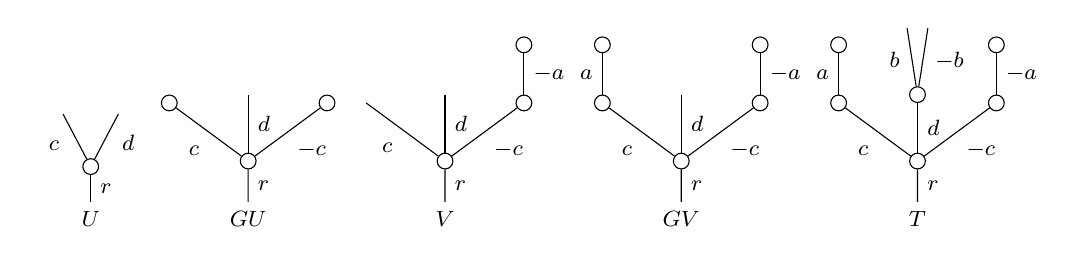
\begin{tikzpicture}[auto,grow=up, every node/.style = {font=\footnotesize}]%
	\begin{scope}[level distance = 1.9em]
	\tikzstyle{level 2}=[sibling distance=2em]%
	\tikzstyle{level 3}=[sibling distance=0.75em]%
		\node at (0,0) {$U$}%
			child{node [dummy] {}%
				child{
				edge from parent node [swap, near end] {$d$}}%
				child{
				edge from parent node [near end] {$\phantom{d}c$}}%
			edge from parent node [swap] {$r$}};%
	\end{scope}
	\begin{scope}[level distance = 2.1em]
	\tikzstyle{level 2}=[sibling distance=2.85em]%
	\tikzstyle{level 3}=[sibling distance=0.75em]%
		\node at (2,0) {$GU$}%
			child{node [dummy] {}%
				child{node [dummy] {}%
				edge from parent node [swap] {$-c$}}%
				child[level distance = 2.4em]{
				edge from parent node [swap] {$d$}}%
				child{node [dummy] {}%
				edge from parent node {$\phantom{-}c$}}%
			edge from parent node [swap] {$r$}};%
		\node at (4.5,0) {$V$}%
			child{node [dummy] {}%
				child{node [dummy] {}%
					child{node [dummy] {}
					edge from parent node [swap] {$-a$}}%
				edge from parent node [swap] {$-c$}}%
				child[level distance = 2.4em]{
				edge from parent node [swap] {$d$}}%
				child{
				edge from parent node {$\phantom{-}c$}}%
			edge from parent node [swap] {$r$}};%
		\node at (7.5,0) {$GV$}%
			child{node [dummy] {}%
				child{node [dummy] {}%
					child{node [dummy] {}
					edge from parent node [swap] {$-a$}}%
				edge from parent node [swap] {$-c$}}%
				child[level distance = 2.4em]{
				edge from parent node [swap] {$d$}}%
				child{node [dummy] {}%
					child{node [dummy] {}
					edge from parent node {$\phantom{-}a$}}%
				edge from parent node {$\phantom{-}c$}}%
			edge from parent node [swap] {$r$}};%
		\node at (10.5,0) {$T$}%
			child{node [dummy] {}%
				child{node [dummy] {}%
					child{node [dummy] {}
					edge from parent node [swap] {$-a$}}%
				edge from parent node [swap] {$-c$}}%
				child[level distance = 2.4em]{node [dummy] {}%
					child{
					edge from parent node [near end,swap]{$-b$}}%
					child{
					edge from parent node [near end]{$\phantom{-}b$}}%
				edge from parent node [swap] {$d$}}%
				child{node [dummy] {}%
					child{node [dummy] {}
					edge from parent node {$\phantom{-}a$}}%
				edge from parent node {$\phantom{-}c$}}%
			edge from parent node [swap] {$r$}};%
	\end{scope}
	\end{tikzpicture}%
\]%

\end{example}

\begin{remark}\label{GINNER REM}
	For any inner face $V-e$ of $V$ one has 
	that $G(V-e)$ is either $GV - Ge$ or $GV$.
	Indeed, the latter will happen iff $V-e$ contains either an inner edge of a leaf of the form $ge$.
\end{remark}








\newpage

\subsection{The characteristic edge set argument}


\begin{definition}\label{CHAREDGE DEF}
Let $T \in \Omega_G$, $X \subseteq \Omega[T]$ a subdendroidal set, and $\{U_i\}_{i \in I} \subseteq \mathsf{Face}(T)$ a subset.

Given a set $\Xi^i$ of inner edges of $U_i$ and a subface $V \hookrightarrow U_i$, denote $\Xi_V^i = \Xi^i \cap E^{\mathsf{i}}(V)$.

Suppose further that the indexing set $I$ is a 
finite $G$-poset. For each $i \in I$ denote
\[
X_{<i} = X \cup \bigcup_{j \colon j<i} \Omega[U_j]
\]
We say that $\{\Xi^i \subseteq E^{\mathsf{i}}(U_i)\}$ 
is a \textit{characteristic inner edge collection of $\{U_i\}$ with respect to $X$} if:
\begin{itemize}
	\item[(Ch0)] $X$, $\{U_i\}$ and $\{\Xi^i\}$ are all $G$-equivariant, i.e. $g X = X$, $g U_i = U_{gi}$, $g \Xi^i = \Xi^{gi}$ as appropriate; 
	\item[(Ch1)] for all $i$, any outer face $V = \bar{V}^{U_i}$
		of $U_i$ such that $\Xi_{V}^i = \emptyset$
		is contained in $X_{<i}$;
	\item[(Ch2)] for all $i$, any face
		$V \hookrightarrow U_i$ such that $(V-\Xi_V^i) \in X$
		is contained in $X_{<i}$;
	\item[(Ch3)] for all $j \not \geq i$, 
		all faces $V \hookrightarrow U_i$ such that 
		$(V-\Xi^i_V) \hookrightarrow U_j$
		are contained in $X_{<i}$.
\end{itemize}
\end{definition}


\begin{remark}\label{XIIII REM}
If $g i \neq i$, then $i,g i$ are incomparable in $I$. Indeed, otherwise $i<gi<g^2i<g^3i<\cdots$ would violate antisymmetry.
Therefore, (Ch3) applies whenever $j=gi$ for $gi\neq i$.

In particular, we assume throughout that if
$gi \neq i$ then $U_{gi} \neq U_i$,
or else it would be $U_i \in X_{<i}$.
\end{remark}


\begin{remark}\label{SOMEMAIN REM}
In some of the main examples (see Propositions \ref{ORB_HORN_PROP} and \ref{REG_HORN_PROP}), there exists a $G$-equivariant set 
$\Xi$ of inner edges of $T$ such that $\Xi^i = \Xi \cap E^{\mathsf{i}}(U_i)$.

%In such cases (Ch3) guarantees that, for fixed $\Xi$ and $X$, the characteristic conditions are monotone on $\{U_i\}$, in the sense that if they hold for $\{U_i\}$ they also hold for all of its subsets. NO LONGER TRUE
	
We caution that, for fixed $X$ and $\{U_i\}$, our characteristic conditions are \textit{not} monotone on such $\Xi$ since increasing $\Xi$ makes (Ch1) more permissive while making (Ch2),(Ch3) more restrictive.
\end{remark}


\begin{lemma}\label{CHAREDGE LEM}
If $\{\Xi^i\}_{i \in I}$ is a characteristic inner edge collection of $\{U_i\}_{i\in I}$ with respect to $X$, then the map
\begin{equation}\label{CHARLEM EQ}
	X \to X \cup \bigcup_{i \in I} \Omega[U_i]
\end{equation}
is $G$-inner anodyne. In fact, it is cellular on $G$-inner horn inclusions $\Lambda^E[S] \to \Omega[S]$, $S \in \Omega_G$.
\end{lemma}


\begin{proof}
We start with the case of $I \simeq G/H$ orbital so that, abbreviating $U = U_{[e]}$, $\{U_i\}$ is the set of conjugates $gU$. 
Note that $H$ is also the isotropy of $U$ in $\mathsf{Face}(T)$.
We likewise abbreviate $\Xi = \Xi^{[e]}$ and
$\Xi_V = \Xi_V^{[e]}$ for $V \hookrightarrow U$.
Moreover, in this case one has $X_{<[g]}=X$ in (Ch1),(Ch2),(Ch3).

We write $\mathsf{Face}_{\Xi}^{lex}(U)$
for the $H$-poset of planar faces $V \hookrightarrow U$
such that $\Xi_V \neq \emptyset$ and $\Xi_V = \Xi_{\bar{V}}$
ordered as follows: 
$V \leq V'$ if either
	\begin{inparaenum}
		\item[(i)] $\bar{V} \hookrightarrow \bar{V}'$ and 
		$\bar{V} \neq \bar{V}'$ or
		\item[(ii)] $\bar{V} = \bar{V}'$ and
		$V \hookrightarrow V'$
	\end{inparaenum}
(alternatively, this is the lexicographic order of pairs $(\bar{V},V))$.
We note that here and in the remainder of the proof all outer closures are implicitly taken in $U$ (rather than $T$), i.e. 
$\bar{V}=\bar{V}^U$.

For any $H$-equivariant convex subset $C$ of $\mathsf{Face}_{\Xi}^{lex}(U)$ we write
\[
X_C = 
X \cup \bigcup_{g\in G,V \in C} \Omega[gV].
\]
It now suffices to show that whenever
$C \subseteq C'$
the map 
$X_C \to X_{C'}$ is built cellularly from 
$G$-inner horn inclusions
(indeed, setting $C=\emptyset$ and 
$C'=\mathsf{Face}_{\Xi}^{lex}(U)$ recovers \eqref{CHARLEM EQ}
when $I \simeq G/H$).

Without loss of generality we can assume that $C'$ is obtained from $C$ by adding the $H$-orbit of a single $W \hookrightarrow U$. Further, we may assume $W \not \in X_C$ or else $X_C=X_{C'}$.
Letting $K \leq H$ denote the isotropy of 
$W$ in $\mathsf{Face}_{\Xi}^{lex}(U)$ and regarding $W \in \Omega^{K}\subseteq \Omega_{K}$, we claim there is a pushout diagram
\begin{equation}\label{FIRPUSH EQ}
\begin{tikzcd}
	G \cdot_{K} \Lambda^{\Xi_{W}}[W] \ar{d} \ar{r}&
	X_C \ar{d}
\\
	G \cdot_{K} \Omega[W] \ar{r}&
	X_{C'}
\end{tikzcd}
\end{equation}
where we note that inner edge set $\Xi_{W}$ is $K$-equivariant
since $\Xi_W = \Xi \cap E^{\mathsf{i}}(W)$ and $\Xi$ is $H$-equivariant by (Ch0).
The desired pushout will follow once we establish the following claims:
\begin{enumerate}
\item[(a)] all outer faces $V$ of $W$ are in $X_C$;
\item[(b)] an inner face $W - D$ of $W$ is in $X_C$ iff 
$D \not \subseteq \Xi_{W}$;
\item[(c)] 
the $G$-isotropy (i.e. the isotropy in $\mathsf{Face}(T)$)
of faces 
$W - D$, $D \subseteq \Xi_{W}$ is contained in $K$.
%the $G$-isotropy of inner faces 
%(i.e. their isotropy in $\mathsf{Face}(T)$)
%is contained in $G_W$.
\end{enumerate}

To check (a), writing $\bar{V}$ for the corresponding outer face of $U$, one has
	\[
	\Xi_V = \Xi \cap E^{\mathsf{i}} (V) 
	= \Xi \cap E^{\mathsf{i}}(W) \cap E^{\mathsf{i}}(\bar{V})
	= \Xi \cap E^{\mathsf{i}}(\bar{W}) \cap E^{\mathsf{i}}(\bar{V})
	= \Xi \cap E^{\mathsf{i}}(\bar{V})
	= \Xi_{\bar{V}}
	\]
where the second step follows from Lemma \ref{INNINT LEM}
(applied to $V \hookrightarrow W \hookrightarrow U$, 
$V \hookrightarrow \bar{V} \hookrightarrow U$)
and the third since by definition of
$\mathsf{Face}_{\Xi}^{lex}(U)$ it is $\Xi_{W} = \Xi_{\bar{W}}$.
Thus either $\Xi_V= \Xi_{\bar{V}} = \emptyset$ so that $\bar{V}\in X$ by (Ch1) 
or $\Xi_V = \Xi_{\bar{V}} \neq \emptyset$
so that $V \in \mathsf{Face}_{\Xi}^{lex}(U)$ with $V<W$, and thus $V\in C$. In either case one has $V \in X_C$.

We now check the ``if'' direction of (b).
If $D \not \subseteq \Xi_{W}$
then $W' = W - (D \setminus \Xi_{W})$
is in $\mathsf{Face}_{\Xi}^{lex}(U)$
(since $\bar{W}' = \bar{W}$ and $\Xi_{W'} = \Xi_{W}$)
and $W'<W$, and thus $W' \in X_C$.

For the ``only if'' direction of (b), the assumption $W \not \in X_C$ together with (Ch2) imply that
$W'=W-\Xi_{W}$ is not in $X$, and hence it remains to show that 
$W'$ is not a face of any $gV$ with $g\in G$, $V \in C$.
Suppose otherwise, i.e. $W' \hookrightarrow gV$.
If it were $g \not \in H$, 
then it would be $W' \hookrightarrow gV \hookrightarrow g U \neq U$, and (Ch3) would imply $W\in X$. Thus we need only consider $g\in H$, and since $C$ is $H$-equivariant, we may as well set $g=e$.
But now since $W' \hookrightarrow V$ it is $ \bar{W} = \bar{W}' \hookrightarrow \bar{V}$
and by convexity of $C'$ it must in fact be 
$ \bar{W} = \bar{V}$. But by definition of 
$\mathsf{Face}_{\Xi}^{lex}(U)$ the face $V$ must contain as inner edges all edges in 
$\Xi_V=\Xi_{\bar{V}} = \Xi_{\bar{W}} = \Xi_{W}$,
so that it is not only $W - \Xi_{W} = W' \hookrightarrow V$ but also $W \hookrightarrow V$.
This contradicts the assumption $W \not \in X_C$.

We now show (c).
If $g(W-D)=W-D$ then $g(W - \Xi_W) \hookrightarrow U$
and thus $W - \Xi_W \hookrightarrow g^{-1}U$,
so that by (Ch3) it must be $g \in H$ or else it would be $W \in X$.
Now suppose $h(W-D)=W-D$ with $h\in H$.
Since $\Xi$ is $H$-equivariant (by (Ch0)) and
$\Xi_{W-D} = \Xi_{W} \setminus D$ (due to $D \subseteq \Xi_{W}$) it follows that 
$h(W-\Xi_W)=W-\Xi_W$,
so that we may assume $D=\Xi_W$.
Now note that
$hW$, $h(W-\Xi_W)=W-\Xi_W$, $W$
are all faces of $U$ with a common outer closure $\bar{W}$.
Hence 
$h\Xi_{W} = \Xi_{hW} \subseteq \Xi_{\bar{W}} = \Xi_{W}$, where the last step follows since
$W \in \mathsf{Face}_{\Xi}^{lex}(U)$, and by cardinality reasons it must in fact be $h \Xi_{W} = \Xi_{W}$. But then $hW,W$
have the same outer closure and the same inner edges, and thus 
$hW=W$, establishing (c).

Lastly, we address the case of general $I$.
For each $G$-equivariant convex subset $J$ of $I$, set
\[
	X_J = 
	X \cup \bigcup_{j \in J} \Omega[U_j].
\]
As before, it suffices to check that for all convex subsets
$J \subseteq J'$
the map $X_J \to X_{J'}$ is built cellularly from $G$-inner horns,
and again we can assume that $J'$ is obtained from $J$ by adding a single $G$-orbit $Gj$ of $I$.
By the $I$ orbital case, it now suffices to check that
$\{\Xi^{gj}\}_{gj \in Gj}$ is also a characteristic inner edge collection of $\{U_{g j}\}_{g j \in Gj}$ with respect to $X_J$.
(Ch0) is then clear, and since by $G$-equivariance and convexity it is $X_{<gj} \subseteq X_J$,
the new (Ch1),(Ch2),(Ch3)
conditions follow from the original conditions.
\end{proof}


\begin{remark}\label{CHAREDGE2 REM}
The requirement $X \subseteq \Omega[T]$ in Definition \ref{CHAREDGE DEF} can be relaxed.
Given an inclusion $X \subseteq Y$,
a set of non-degenerate dendrices
$\{y_i \in Y(U_i)\}_{i \in I}$
and a collection of edges
$\{\Xi^i \subset E^{\mathsf{i}}(U_i)\}_{i \in I}$, 
suppose that $I$ is a finite $G$-poset and that:
\begin{itemize}
	\item[(Ch0.1)] the maps $y_i \colon \Omega[U_i] \to Y$ are monomorphisms;
	\item[(Ch0.2)] $X$, $\{U_i\}$ ,$\{y_i\}$ and $\{\Xi^i\}$
	are all $G$-equivariant in the sense that:
	\begin{inparaenum}
	\item[(i)] $gX = X$;
	\item[(ii)] there are associative and unital isomorphisms
	$U_i \xrightarrow{g} U_{g_i}$;
	\item[(iii)] the composites
	$\Omega[U_i] \xrightarrow{y_i} Y \xrightarrow{g} Y$
	and
	$\Omega[U_i]  \xrightarrow{g} \Omega[U_{gi}] \xrightarrow{y_{gi}} Y$ coincide;
	\item[(iv)] $g \Xi^i=\Xi^{gi}$.
\end{inparaenum}
	 
%	\item[(Ch0*3)] for each face $V \hookrightarrow U_i$ and $g \in G$
%	then $g y_i(V) = y_i(V)$ implies 
%	$g y_i(\bar{V}) = y_i(\bar{V})$.
\end{itemize}
Under (Ch0.1),
the $\Omega[U_i]$ are identified with subcomplexes of $Y$,
and non-degenerate dendrices $y \in y_i(\Omega[U_i])(V)$
are identified with faces $V \hookrightarrow U_i$.

The original conditions (Ch1),(Ch2),(Ch3) can then be reinterpreted by, 
for each $V \hookrightarrow U_i$, 
regarding expressions such as $V \in X$, $(V-\Xi^i_V)\in U_j$
as $y_i(V) \in X$, $y_i(V-\Xi^i_V) \in y_j(\Omega[U_j])$.

The proof of Lemma \ref{CHAREDGE DEF} now carries out to show that 
\begin{equation}
	X \to X \cup \bigcup_{i \in I} y_i(\Omega[U_i])
\end{equation}
is $G$-inner anodyne (again built cellularly from $G$-inner horn inclusions).
%hence we note only the main differences.
%When writing the analogue of (\ref{FIRPUSH EQ}), 
%$K$ must be defined by noting that, cf. Remark \ref{FACEGACT REM},
%the $G \times \mathsf{Aut}(W)$-isotropy of 
%$y(W) \in y(\Omega[U])$
%is the graph of some partial homomorphism
%$G \geq K \xrightarrow{\phi} \mathsf{Aut}(W)$.
%Hence, when stating and proving the analogue of (c) one must instead deal with
%$G \times \mathsf{Aut}(W)$ and $G \times \mathsf{Aut}(W-D)$-isotropies.
%However, as explained in Remark \ref{FACEGACT REM}, the role of the $\mathsf{Aut}(W)$ and $\mathsf{Aut}(W-D)$ coordinates is simply to implement the replanarization isomorphism in (\ref{FACEGACT EQ}). 
%Hence, since non-degenerate $y' \in y(\Omega[U])$ are identified with faces in $\Omega^+\downarrow U$, by borrowing the notation in 
%Remark \ref{PLFUNCTOR REM}, the analogue of (c) states that if
%$pl(g y (W-D)) = y(W-D)$ then $pl(g y (W)) = y(W)$ 
%(note that $y(W)=pl(y(W))$ by definition of $W$).
%But reinterpreting the argument in the proof of Lemma \ref{CHAREDGE DEF}
%shows that $pl(g^{-1} y (W)),y(W)$ are planar faces of $U$ with the same closure and the same edges, and hence indeed 
%$pl(g y (W))=y(W)$.
\end{remark}

%\begin{example}
%To see the need for condition (Ch0*3),
%let $Y =\Delta[2] \amalg_{d_1(\Delta[1])} \Delta[2]$,
%where $d_1 \colon \Delta[1] \to \Delta[2]$
%is the inner face,
%together with the obvious $\mathbb{Z}_{/2}$-action.
%Then for $X = \Lambda^1[2] \amalg_{\partial \Delta[1]} \Lambda^1[2]$ and
%$\{y_i\}$ (resp. $\Xi$) the $\mathbb{Z}_{/2}$-orbital set
%consisting of the two copies of $\Delta[2]$ (resp. two copies of 
%$1 \in \Delta[2]$), 
%conditions (Ch0*1),(Ch0*2),(Ch1),(Ch2),(Ch3) all hold while (Ch0*3) fails,
%and one easily sees that $X \to Y$ is not built cellularly from 
%$\mathbb{Z}_{/2}$-inner horns.
%\end{example}


\begin{remark} Lemma \ref{CHAREDGE LEM} readily recovers several arguments in the literature:
\begin{itemize}
\item[(i)] In \cite[\S 10]{Rez01} (also \cite[\S 6.2]{Rez10}), Rezk introduces the notion of \textit{covers}, which in our language are the subsets
$Sc[n] \subseteq X \subseteq \Delta[n]$
such that if $V$ is in $X$ then so is the closure $\bar{V}^{[n]}$
(in words, $X$ is generated by outer faces).
Similarly, in the proof of \cite[Prop. 2.4]{CM13a}
Cisinski and Moerdijk use subcomplexes $S_j$ that can be regarded as
\textit{dendroidal covers},
i.e. subcomplexes
$Sc[T] \subseteq X \subseteq \Delta[T]$
such that if $V$ is in $X$ then so is $\bar{V}^{T}$.
Lastly, the subcomplexes 
$\Omega[T] \cup_l \Omega[S] \subseteq \Omega[T \circ_l S]$
in the grafting result \cite[Lemma 5.2]{MW09} (and similarly for the equivariant analogue \cite[Prop. 6.19]{Per17}) are also dendroidal covers.

It follows from Lemma \ref{CHAREDGE LEM}
that any inclusion $X \to X'$ of $G$-equivariant (dendroidal) covers of $T\in \Omega_G$
is $G$-inner anodyne. 
Indeed, letting $I=\mathsf{Face}_{X'}^{out}(T)$ be the $G$-poset of outer faces $V \hookrightarrow T$, ordered by inclusion, 
$\Xi = E^{\mathsf{i}}(T)$ and $U_V = V$,
(Ch0) is obvious, (Ch1) follows since 
$Sc(T) \subseteq X$, (Ch2) follows since $X$ is a cover and
(Ch3) follows since the $U_i$ are closed.

Alternatively, one can also use $I=\mathsf{Face}_{X',o}^{out}(T)$
for the $G$-trivial set (viewed as a \textit{discrete} poset)
of orbital outer faces $GV \to T$ (see Remark \ref{TWOPROOF REM} for a similar example).

Lastly, we note that if $\{U_i\}=\{T\}$, $\Xi=E^{\mathsf{i}}(T)$
then (Ch1) says precisely that $Sc(T) \subseteq X$.


\item[(ii)] In \cite[Lemma 9.7]{MW09}, Moerdijk and Weiss introduced a \textit{characteristic edge} condition that can be regarded as a special case of our characteristic edge collection condition as generalized in Remark \ref{CHAREDGE2 REM}, and was one of our main inspirations.

Therein, they work in the case of $Y= \Omega[T] \otimes \Omega[S]$
a tensor product of (non-equivariant) representable dendroidal sets, in which case (Ch0.1) is easily verified (and (Ch0.2) is moot).
In our notation, they then require that $I \simeq \**$ (so that (Ch3) is also moot), 
the dendrex 
$y_{\**} \in \left(\Omega[T] \otimes \Omega[S]\right)(U_{\**})$ encodes a special type of subtree $U_{\**}$ of $\Omega[T] \otimes \Omega[S]$, which they call an \textit{initial segment},
and they further require that $\Xi^{\**} = \{\xi\}$ is a singleton, called the \textit{characteristic edge}.
Moreover, they then demand that $X$ should contain all outer faces of the subtree $U_{\**}$, from which (Ch1) follows, 
as well as the key characteristic condition 
\cite[Lemma 9.7]{MW09}(ii),
which coincides with (Ch2) in this specific setting.

Similarly, in \cite[Lemma 7.39]{Per17} the second author introduced a \textit{characteristic edge orbit} condition that generalizes that in \cite{MW09} to the equivariant context 
by letting $I \simeq G/H$
and the $\Xi^{[g]}=\Xi \cap E^{\mathsf{i}}(U_{[g]})$ be determined by a $G$-edge orbit $\Xi \simeq Gf$ (cf. Remark \ref{SOMEMAIN REM}).

However, both of the lemmas in \cite{MW09} and \cite{Per17}
have the drawback of needing to be used iteratively
(so that much effort therein is spent showing that this can be done) while Lemma \ref{CHAREDGE LEM} is designed so that a single use suffices for the natural applications.
Indeed, conditions (Ch1) and (Ch3), the first of which relaxes the requirement in \cite{MW09},\cite{Per17} that $X$ should contain all outer faces, essentially provide abstract conditions under which the original characteristic edge arguments of \cite{MW09},\cite{Per17} can be iterated.
%Further, we note that in \cite{MW09},\cite{Per17} it is essential to make a good choice for the well-ordering in (Ch3).
%
%We end by noting the importance of the $G$-equivariance of $\Xi$
%in (Ch0),(Ch0*2). In proving \cite[Prop. 7.44]{Per17} the second author chose the $\Xi$ to be sets of edges of the subtrees $y_i$, and thus not necessarily $G$-equivariant,
%leading to the need of extra ad hoc arguments in that proof when establishing the analogue of condition (c) in the proof of Lemma \ref{CHAREDGE LEM}.
\end{itemize}
\end{remark}

{\color{red}HERE}

\begin{example}
	As indicated above, Lemma \ref{CHAREDGE LEM} can be used to
	reorganize and streamline the rather long proofs of \cite[Thms 7.1 and 7.2]{Per17}. We illustrate this in the hardest case, that of \cite[Thm. 7.1(i)]{Per17}, which states that if
	$S,T \in \Omega_G$ are open (i.e. have no stumps) and
	$G \xi$ is an inner edge orbit of $T$ the maps
\begin{equation}\label{THM71 EQ}
	\partial \Omega[S] \otimes \Omega[T]
		\coprod_{\partial \Omega[S] \otimes \Lambda^{G\xi}[T]}
	\Omega[S] \otimes \Lambda^{G\xi}[T]
\to
	 \Omega[S] \otimes \Omega[T]
\end{equation}
are $G$-inner anodyne.

As detailed in \cite[\S 5.1]{Per17},
and originally due to Weiss in \cite{Wei12},
there is an algebraically flavoured model for $\Omega$
as certain types of \textit{broad posets}.
Given $S,T \in \Omega_G$, it is then possible \cite[\S 7.1]{Per17} to define a $G$-equivariant broad poset $S \otimes T$
so that 
$\left(\Omega[S] \otimes \Omega[T]\right)(V) = Hom(V,S \otimes T)$
where the Hom set is taken in broad posets.

\cite[Thm. 7.1(i)]{Per17} now follows from Lemma \ref{CHAREDGE LEM} by letting $I = \mathsf{Max}^{lex}(S \otimes T)$
be the poset of maximal subtrees $U \hookrightarrow S \otimes T$ 
(these are called \textit{percolation schemes} in \cite[\S 9]{MW09}) ordered lexicographically \cite[Def. 7.29]{Per17}.

{\color{red}HERE}

$\Xi = \{(s,g\xi) \in S\otimes T\}$.

{\color{blue} Does not quite follow from this Lemma \ref{}
e original argument, need $\Xi^{[i]}$}.



(Ch3) is almost literally the content of \cite[Lemma 3.37]{Per17}.

\end{example}








\newpage


\appendix

\section{Equivariant Reedy model structures}


{\color{blue} Bla bla one of the axioms in \cite{BM11} is different from the others point of view}

In \cite{BM11} Berger and Moerdijk extend the notion of Reedy category so as to allow for categories $\mathbb{R}$
 with non-trivial automorphism groups 
 $\mathsf{Aut}(r)$ for $r \in \mathbb{R}$.
For such $\mathbb{R}$ and suitable model category $\mathcal{C}$ they then show that there is a 
\textit{Reedy model structure}
on $\mathcal{C}^{\mathbb{R}}$
that is defined by modifying the usual characterizations of
Reedy cofibrations, weak equivalences and fibrations
(see \cite[Thm. 1.6]{BM11} or
Theorem \ref{REEDYADM THM} below)
 to be determined by the $\mathsf{Aut}(r)$-projective model structures
on $\mathcal{C}^{\mathsf{Aut}(r)}$
for each $r \in \mathbb{R}$. 

The purpose of this appendix is to show that,
under suitable conditions, this can also be done by replacing
the $\mathsf{Aut}(r)$-projective model structures
on $\mathcal{C}^{\mathsf{Aut}(r)}$
with the more general 
$\mathcal{C}^{\mathsf{Aut}(r)}_{\mathcal{F}_r}$
model structures for 
$\{\mathcal{F}_r\}_{r \in \mathbb{R}}$
a nice collection of families of subgroups of each 
$\mathsf{Aut}(r)$.

To do so, we first need some essential notation.
For each map $r \to r'$ in a category $\mathbb{R}$ we will write
$\mathsf{Aut}(r \to r')$ for its automorphim group in the arrow category and write
\begin{equation}\label{PIDEFR EQ}
\begin{tikzcd}
\mathsf{Aut}(r) &
\mathsf{Aut}(r \to r') \ar{r}{\pi_{r'}} \ar{l}[swap]{\pi_{r}} &
\mathsf{Aut}(r')
\end{tikzcd}
\end{equation}
for the obvious projections. We now introduce our equivariant generalization of
the ``generalized Reedy categories''
of \cite[Def. 1.1]{BM11}.

\begin{definition}\label{GENRED DEF}
A \textit{generalized Reedy category structure} on a
small category $\mathbb{R}$ consists of
wide subcategories 
$\mathbb{R}^+$, $\mathbb{R}^-$
and a degree function $|\minus| \colon ob(\mathbb{R}) \to \mathbb{N}$ such that:
\begin{itemize}
	\item[(i)] non-invertible maps in $\mathbb{R}^+$ (resp. $\mathbb{R}^-$) raise (lower) degree; isomorphisms preserve degree;
	\item[(ii)] $\mathbb{R}^+ \cap \mathbb{R}^- = \mathsf{Iso}(\mathbb{R})$;
	\item[(iii)] every map $f$ in $\mathbb{R}$ factors as
	$f = f^{+} \circ f^{-}$ with $f^{+} \in \mathbb{R}^+$, $f^{-} \in \mathbb{R}^-$, and this factorization is unique up to isomorphism.
\end{itemize}
Let $\{\mathcal{F}_r\}_{r \in \mathbb{R}}$
be a collection of families of subgroups of the groups $\mathsf{Aut}(r)$.
The collection $\{\mathcal{F}_r\}$ is called 
\textit{Reedy-admissible} if:
\begin{itemize}
	\item[(iv)] for all maps
	$r \twoheadrightarrow r'$ in $\mathbb{R}^-$ one has
	$\pi_{r'}\left( \pi_r^{-1} (H) \right) \in \mathcal{F}_{r'}$
	for all $H \in \mathcal{F}_r$.
\end{itemize}
\end{definition}

We note that condition (iv) above should be thought as of a constraint on the pair 
$(\mathbb{R},\{\mathcal{F}_r\})$.
The original setup of \cite{BM11} then deals with the case
where $\{ \mathcal{F}_r \} =
 \left\{ \left\{ e \right\} \right\}$
is the collection of trivial families. Indeed, our setup recovers
the setup in \cite{BM11}, as follows.

\begin{example}
	When $\{ \mathcal{F}_r \} =
 \left\{ \left\{ e \right\} \right\}$, Reedy-admissibility coincides with axiom (iv) in \cite[Def. 1.1]{BM11},
stating that if $\theta \circ f^{-} = f^{-}$
for some $f^- \in \mathbb{R}^{-}$ and 
$\theta \in \mathsf{Iso}(\mathbb{R})$ then $\theta$ is an identity.
\end{example}

\begin{example}
For any generalized Reedy category $\mathbb{R}$, the collection $\{\mathcal{F}_{\text{all}}\}$
of the families of all subgroups of $\mathsf{Aut}(r)$
is Reedy-admissible.
\end{example}

\begin{example}
	Let $G$ be a group and set $\mathbb{R} = G \times (0 \to 1)$ with $\mathbb{R} = \mathbb{R}^+$. Then any pair 
	$\{\mathcal{F}_0,\mathcal{F}_1\}$
	of families of subgroups of $G$ is Reddy-admissible.
	
	Similarly, set $\mathbb{S} = G \times (0 \leftarrow 1)$
	with $\mathbb{S} = \mathbb{S}^-$. Then a pair
	$\{\mathcal{F}_0,\mathcal{F}_1\}$
	of families of subgroups of $G$ is Reddy-admissible
	iff $\mathcal{F}_0 \supset \mathcal{F}_1$.
\end{example}


\begin{example}\label{GGRAPHREEDY EX}
	Letting $\mathbb{S}$ denote any generalized Reedy category in the sense of \cite[Def. 1.1]{BM11} and $G$ a group,
	we set $\mathbb{R} = G \times \mathbb{S}$
	with $\mathbb{R}^+ = G \times \mathbb{S}^+$ and 
	$\mathbb{R}^- = G \times \mathbb{S}^+$.
	Further, for each $s \in \mathbb{S}$ we write
	$\mathcal{F}_s^{\Gamma}$ for the family of 
	$G$-graph subgroups of $G \times \mathsf{Aut}_{\mathbb{S}}(s)$, i.e., those subgroups 
	$K \leq G \times \mathsf{Aut}_{\mathbb{S}}(s)$ such that $K \cap \mathsf{Aut}_{\mathbb{S}}(s) = \{e\}$.
	
	Reedy admissibility of $\{\mathcal{F}_s^{\Gamma}\}$ follows since for every degeneracy map 
	$s \twoheadrightarrow s'$ in $\mathbb{S}^-$ one has that the homomorphism
	$\pi_s \colon \mathsf{Aut}_{\mathbb{S}}(s \twoheadrightarrow s')
	\to \mathsf{Aut}_{\Omega}(s)$ is injective
	(we note that this is equivalent to axiom (iv) in \cite[Def. 1.1]{BM11} for $\mathbb{S}$).
\end{example}

Our primary example of interest will come by setting
$\mathbb{S} = \Omega^{op}$ in the previous example.
In fact, in this case we will also be interested 
in certain subfamilies
$\{\mathcal{F}_U\}_{U \in \Omega}
\subset \{\mathcal{F}_U^{\Gamma}\}_{U \in \Omega}$.

\begin{example}
	Let $\mathbb{R} = G \times \Omega^{op}$ and let
	$\{\mathcal{F}_U\}_{U \in \Omega}$ be the family of graph subgroups determined by a weak indexing system $\mathcal{F}$.
	Then $\{\mathcal{F}_U\}$ is Reedy-admissible.
	To see this, recall first that each $K \in \mathcal{F}_U$ encodes 
	an $H$-action on $U \in \Omega$ for some $H \leq G$
	so that $G \cdot_H U$ is a $\mathcal{F}$-tree.
	Given a face map $f \colon U' \hookrightarrow U$, 
	the subgroup $\pi^{-1}_U(K)$ is then determined by the largest subgroup $\bar{H}\leq H$ such that 
	$U'$ inherits the $\bar{H}$-action from $U$ along $f$ (so that $f$ becomes a $\bar{H}$-map), 
	so that $\pi_{U'}(\pi^{-1}_U(K))$ encodes the $\bar{H}$-action on $U'$. Thus, we see that Reedy-admissibility is simply the sieve condition for the induced map of $G$-trees
	$G \cdot_{\bar{H}} U' \to G \cdot_H U$.
\end{example}

We now state the main result.
We will assume throughout that $\mathcal{C}$ is a model category such that for any group $G$ and family of subgroups $\mathcal{F}$,
the category $\mathcal{C}^G$ admits the
$\mathcal{F}$-model structure
(for example, this is the case whenever $\C$ is a cofibrantly generated cellular model category in the sense of \cite{Ste16}).


\begin{theorem}\label{REEDYADM THM}
Let $\mathbb{R}$ be generalized Reedy and 
$\{\mathcal{F}_r\}_{r \in \mathbb{R}}$ a Reedy-admissible collection of families. 
Then there is a \textbf{$\{\mathcal{F}_r\}$-Reedy model structure} on
$\mathcal{C}^{\mathbb{R}}$ such that a map $A \to B$ is
\begin{itemize}
  \item a (trivial) cofibration if $A_r \underset{L_r A}{\coprod}L_r B \to B_r$ is a (trivial) $\mathcal{F}_r$-cofibration in $\mathcal{C}^{\mathsf{Aut}(r)}$, $\forall r \in \mathbb{R}$;
	\item a weak equivalence if $A_r \to B_r$ is a $\mathcal{F}_r$-weak equivalence in $\mathcal{C}^{\mathsf{Aut}(r)}$, $\forall r \in \mathbb{R}$;
	\item a (trivial) fibration if $A_r \to B_r \underset{M_r B}{\times }M_r A $ is a (trivial) $\mathcal{F}_r$-fibration in $\mathcal{C}^{\mathsf{Aut}(r)}$, $\forall r \in \mathbb{R}$.
\end{itemize}
\end{theorem}

The proof of this result is given at the end of the section after establishing some routine generalizations of the key lemmas in \cite{BM11}
(indeed, the true novelty in this appendix is the Reedy-admissibility condition in part (iv) of Definition \ref{GENRED DEF}).

We first recall the following, cf. \cite[Props. 6.5 and 6.6]{BP17}
(we note that \cite[Prop. 6.6]{BP17} can be proven in terms of fibrations, and thus does not depend on special assumptions on $\C$).
\begin{proposition}
Let $\phi \colon G \to \bar{G}$ be a homomorphism and
$\mathcal{F}$, $\bar{\mathcal{F}}$ families of subgroups of
$G, \bar{G}$. Then the leftmost (resp. rightmost) adjunction below
is a Quillen adjunction 
\[
	\bar{G} \cdot_G (\minus)
	\colon \C^G_{\mathcal{F}}
		\rightleftarrows
	\C^{\bar{G}}_{\bar{\mathcal{F}}} \colon
	\mathsf{res}^{\bar{G}}_G
\qquad
	\mathsf{res}^{\bar{G}}_G
	\colon	\C^{\bar{G}}_{\bar{\mathcal{F}}}
		\rightleftarrows
	\C^G_{\mathcal{F}} \colon
	\mathsf{Hom}_G(\bar{G},\minus)
\]
provided that for $H \in \mathcal{F}$ it is
$\phi(H) \in \bar{\mathcal{F}}$
(resp. for $\bar{H} \in \bar{\mathcal{F}}$ it is
$\phi^{-1}(H) \in \mathcal{F}$).
\end{proposition}



\begin{corollary}\label{RESGEN COR}
For any homomorphism $\phi \colon G \to \bar{G}$, the functor
$\mathsf{res}^{\bar{G}}_G \colon 
\C^{\bar{G}} \to \C^G$
preserves all four classes of genuine cofibrations, trivial cofibrations, fibrations and trivial fibrations.
\end{corollary}

The following formalizes an argument implicit in the proof of \cite[Lemma 5.2]{BM11}).

\begin{definition}
Consider a commutative diagram
\begin{equation}\label{BLA EQ}
	\begin{tikzcd}
		A \ar{r} \ar{d} & X \ar{d}
	\\
		B \ar{r} \ar[dashed]{ru} & Y
	\end{tikzcd}
\end{equation}
in $\C^{\mathbb{R}}$. A collection of maps 
$f_s \colon B_s \to X_s$ for $|s|\leq n$ 
that induce a lift of the restriction of \eqref{BLA EQ}
 to $\C^{\mathbb{R}_{\leq n}}$ will be called a 
\textit{$n$-partial lift}. 
\end{definition}


\begin{lemma}\label{BLALIFT LEM}
	Let $\C$ be any bicomplete category, and consider a commutative diagram as in \eqref{BLA EQ}. Then any $(n-1)$-partial lift uniquely induces commutative diagrams
\begin{equation}\label{BLALIFT EQ}
	\begin{tikzcd}
		A_r \amalg_{L_r A} L_r B \ar{r} \ar{d} & X_r \ar{d}
	\\
		B_r \ar{r} \ar[dashed]{ru} & Y_r \times_{M_r Y} M_r X
	\end{tikzcd}
\end{equation}
in $\mathcal{C}^{\mathsf{Aut}(r)}$
for each $r$ such that $|r|=n$. Furthermore, extensions of the 
$(n-1)$-partial lift to a $n$-partial lift are in bijection with choices of $\mathsf{Aut}(r)$-equivariant lifts of the diagrams \eqref{BLALIFT EQ} for $r$ ranging over representatives of the isomorphism classes of $r$ with $|r|=n$.
\end{lemma}

In the next result, by $\{\mathcal{F}_r\}$-cofibration/trivial cofibration/fibration/trivial fibration 
we mean a map as described in 
Theorem \ref{REEDYADM THM}, regardless of whether such a model structure exists.

\begin{corollary}\label{BLALIFT COR}
Let $\mathbb{R}$ be generalized Reedy and 
$\{\mathcal{F}_r\}$ an arbitrary family of subgroups of $\mathsf{Aut}(r)$, $r \in \mathbb{R}$.
Then a map in $\mathcal{C}^{\mathbb{R}}$ 
is a $\{\mathcal{F}_r\}$-cofibration (resp. trivial cofibration) iff it has the left lifting property 
with respect to all 
$\{\mathcal{F}_r\}$-trivial fibrations (resp. fibrations),
and vice-versa for the right lifting property.
\end{corollary}

\begin{lemma}\label{GINJ LEM}
Let $\mathbb{S}$ be a generalized Reedy with $\mathbb{S}=\mathbb{S}^+$, $K$ a group, and $\pi \colon \mathbb{S} \to K$
a functor.

Then if a map $A \to B$ in $\C^{\mathbb{S}}$ is such that for all 
$s \in \mathbb{S}$
the maps 
$
  A_s \amalg_{L_s A} L_s B \to B_s
$	
are (resp. trivial) $\mathsf{Aut}(s)$-cofibrations one has that
$\mathsf{Lan}_{\pi\colon \mathbb{S} \to K}(A \to B)$
is a (trivial) $K$-cofibration.
\end{lemma}

\begin{proof}
By adjunction, one needs only show that for any 
$K$-fibration $X \to Y$ in $\mathcal{C}^K$,
the map $\pi^{\**}(X \to Y)$
has the right lifting property against all maps $A \to B$ in $\C^{\mathbb{S}}$ as in the statement.
By Corollary \ref{BLALIFT COR}, it thus suffices to check
that the maps
\[
	(\pi^{\**} X)_s \to 
	(\pi^{\**} Y)_s \times_{M_s \pi^{\**} Y} M_s \pi^{\**} X
\]
are $\mathsf{Aut}(s)$-fibrations. But since $M_s Z = \**$ 
(recall $\mathbb{S}=\mathbb{S}^+$)
this map is just $X \to Y$ with the $\mathsf{Aut}(s)$-action induced by
$\pi \colon \mathsf{Aut}(s) \to K$, hence 
Corollary \ref{RESGEN COR} finishes the proof.
\end{proof}


\begin{lemma}\label{GINJMIN LEM}
Let $\mathbb{S}$ be a generalized Reedy with $\mathbb{S}=\mathbb{S}^-$, $K$ a group, and $\pi \colon \mathbb{S} \to K$
a functor.

Then if a map $X \to Y$ in $\C^{\mathbb{S}}$ is such that for all 
$s \in \mathbb{S}$
the maps 
$
	X_s \to Y_s \times_{M_s Y} M_s X
$	
are (resp. trivial) $\mathsf{Aut}(s)$-fibrations one has that
$\mathsf{Ran}_{\pi\colon \mathbb{S} \to K}(A \to B)$
is a (trivial) $K$-fibration.
\end{lemma}

\begin{proof}
This follows dually to the previous proof.
\end{proof}

\begin{remark}
Lemmas \ref{GINJ LEM} and \ref{GINJMIN LEM} generalize key parts of the proofs of \cite[Lemmas 5.3 and 5.5]{BM11}.  
The duality of their proofs reflects the duality in 
Corollary \ref{RESGEN COR}.
\end{remark}

\begin{remark}
	Lemma \ref{GINJ LEM} will be applied when
	$K \leq \mathsf{Aut}_{\mathbb{R}}(r)$ and
	$\mathbb{S} = K \ltimes \mathbb{R}^+(r)$ for $\mathbb{R}$ a given generalized Reedy category and $r \in \mathbb{R}$.
	Similarly, Lemma \ref{GINJMIN LEM} will be applied when
	$\mathbb{S} = K \ltimes \mathbb{R}^-(r)$.
	It is straightforward to check that in the $\mathbb{R}^+$ (resp. $\mathbb{R}^-$) case
	maps in $\mathbb{S}$ can be identified with squares as on the left (right)
	\begin{equation}
	\begin{tikzcd}
		r' \ar{r}{+} \ar{d}[swap]{+} & r \ar{d}{\simeq}
	& &
		r \ar{r}{-} \ar{d}[swap]{\simeq} & r' \ar{d}{-}
	\\
		r'' \ar{r}[swap]{+} & r
	& &
		r \ar{r}[swap]{-} & r''
	\end{tikzcd}
\end{equation}
such that the maps labelled $+$ are in $\mathbb{R}^+$,
maps labelled $-$ are in $\mathbb{R}^-$,
the horizontal maps are non-invertible, and the maps labeled $\simeq$ are automorphisms in $K$. 

In particular, there is thus a \textit{domain} (resp. \textit{target}) functor
$d \colon \mathbb{S} \to \mathbb{R}$ 
($t \colon \mathbb{S} \to \mathbb{R}$), and our interest is in maps  
$d^{\**}A \to d^{\**} B$
($t^{\**}A \to t^{\**} B$) in $\mathcal{C}^{\mathbb{S}}$
induced from maps
$A \to B$ in $\C^{\mathbb{R}}$ so that
\[\mathsf{Lan}_{\pi} d^{\**} (A \to B) = 
(L_r A \to L_r B)
	\qquad
\mathsf{Ran}_{\pi} t^{\**} (A \to B) = 
(M_r A \to M_r B)
\]
\end{remark}

We are now in a position to prove the following, which are the essence of Theorem \ref{REEDYADM THM}.

\begin{lemma}\label{REEDYTRCOF LEM}
Let $\mathbb{R}$ be generalized Reedy and 
$\{\mathcal{F}_r\}_{r \in \mathbb{R}}$ a Reedy-admissible family.

Suppose $A \to B$ be a $\{\mathcal{F}_r\}$-Reedy cofibration. Then the maps $A_r \to B_r$ are all $\{\mathcal{F}_r\}$-weak equivalences iff so are the maps $A_r \amalg_{L_r A} L_r B \to B_r$.
\end{lemma}

\begin{proof}
It suffices to check by induction on $n$ that the analogous claim with the restriction $|r|\leq n$ also holds. The $n=0$ case is obvious. Otherwise, letting $r$ range over representatives of the isomorphism classes of $r$ with $|r|=n$,
it suffices to check that for each $H \in \mathcal{F}_r$
the map
$A_r \to B_r$ is a $H$-genuine weak equivalence iff 
so is $A_r \amalg_{L_r A} L_r B \to B_r$.

One now applies Lemma \ref{GINJ LEM} with 
$K = H$ and 
$\mathbb{S} = H \ltimes \mathbb{R}^+(r)$
to the map $d^{\**}A \to d^{\**}B$. Note that $\mathcal{F}$-trivial cofibrations are always genuine trivial cofibrations, for any family, so that the trivial cofibrancy requirements are immediate from Corollary \ref{RESGEN COR}. 
It thus follows that the maps labelled $\sim$
\[
\begin{tikzcd}[row sep=10]
   L_r A \ar{r}{\sim} \ar[d]   & 
   L_r B \ar[d] & 
\\
   A_r \ar{r}[swap]{\sim}& L_T B \amalg_{L_T A} A_T \ar{r} &
   B_r
\end{tikzcd}
\]
are $H$-genuine trivial cofibrations, finishing the proof.
\end{proof}

\begin{lemma}\label{REEDYTRFIB LEM}
Let $\mathbb{R}$ be generalized Reedy and 
$\{\mathcal{F}_r\}_{r \in \mathbb{R}}$ a Reedy-admissible family.

Let $X \to Y$ be a $\{\mathcal{F}_r\}$-Reedy fibration. Then the maps $X_r \to Y_r$ are all $\{\mathcal{F}_r\}$-weak equivalences iff so are the maps $X_r \to Y_r \times_{M_r Y} M_r X$.
\end{lemma}

\begin{proof}
One repeats the same induction argument on $|r|$.
In the induction step, it suffices to verify that, for each $r$ with $|r|=n$ and $H \in \mathcal{F}_r$, the map
$X_r \to Y_r$ is a $H$-genuine weak equivalence iff 
so is $X_r \to Y_r \times_{M_r Y} M_r X$.

One now applies Lemma \ref{GINJMIN LEM} with 
$K = H$ and 
$\mathbb{S} = H \ltimes \mathbb{R}^-(r)$
to the map $t^{\**}A \to t^{\**}B$. 
Note that for each $(r \twoheadrightarrow r') \in \mathbb{S}$ one has $\mathsf{Aut}_{\mathbb{S}}(r \to r') = \pi_r^{-1}(H)$
(where $\pi_r$ is as in \eqref{PIDEFR EQ}), so that the trivial fibrancy requirement in Lemma \ref{GINJMIN LEM} follows from 
$\{\mathcal{F}_r\}$ being Reedy-admissible.
It follows that the maps labelled $\sim$
\[
\begin{tikzcd}[row sep=10]
	X_r \ar{r}&
	Y_r \times_{M_r Y} M_r X \ar[d] \ar{r}{\sim} & 
	Y_r \ar[d]
\\
	&
	M_r X \ar{r}[swap]{\sim}&
	M_r Y
\end{tikzcd}
\]
are $H$-genuine trivial fibrations, finishing the proof.
\end{proof}

\begin{remark}
The proofs of Lemmas \ref{REEDYTRCOF LEM} and \ref{REEDYTRFIB LEM}
are similar, but not dual, since
Lemma \ref{REEDYTRFIB LEM} uses Reedy-admissibility 
while Lemma \ref{REEDYTRCOF LEM} does not.
This reflects the difference in the proofs of 
\cite[Lemmas 5.3 and 5.5]{BM11} as discussed in 
\cite[Remark 5.6]{BM11}, albeit with a caveat.

Setting $K=\{e\}$ in Lemma \ref{GINJ LEM} yields that
$\mathsf{lim}_{\mathbb{S}} (A \to B)$ is a cofibration provided that $A \to B$ is a genuine Reedy cofibration, i.e. a Reedy cofibration for $\{\mathcal{F}_{\text{all}}\}$ the families of all subgroups. 
On the other hand, the proof of \cite[Lemma 5.3]{BM11} argues that 
$\mathsf{lim}_{\mathbb{S}} (A \to B)$ is a cofibration provided that $A \to B$ is a projective Reedy cofibration, i.e. a Reedy cofibration for $\{\{e\}\}$ the trivial families 
(note that all projective cofibrations are genuine cofibrations, so that our claim is more general).
Since the cofibration half of the projective analogue of Corollary \ref{RESGEN COR} only holds if $\phi$ is a monormorphism, the argument in the proof of \cite[Lemma 5.3]{BM11} also includes an injectivity check that is not needed for our proof of Lemma \ref{REEDYTRCOF LEM}.
\end{remark}


\begin{proof}[proof of Theorem \ref{REEDYADM THM}]
Lemmas \ref{REEDYTRCOF LEM} and \ref{REEDYTRFIB LEM} say that the characterizations of trivial cofibrations (resp. trivial fibrations) in the statement of Theorem \ref{REEDYADM THM} are correct, i.e. that they describe the maps that are both cofibrations (resp. fibrations) and weak equivalences.	

	We refer to the model category axioms in \cite[Def. 1.1.3]{Hov99}. 	
	Both 2-out-of-3 and the retract axioms are immediate
(recall that retracts commute with limits/colimits).	
	The lifting axiom follows from Corollary \ref{BLALIFT COR}
	while the task of building factorizations $X \to A \to Y$ of a given map $X \to Y$ follows by a similar standard argument by iteratively factorizing the maps
\[
	X_r \amalg_{L_r X} L_r A \to Y_r \times_{M_r Y} M_r A
\]
in $\mathcal{C}^{\mathsf{Aut}(r)}$, 
thus building both $A$ and the factorization inductively (see, e.g., the proof of \cite[Thm. 1.6]{BM11}).
\end{proof}



%\section{Even more characteristic edge arguments}



%In the next result recall that 
%$y_i \in Y(U_i)$ means $y_i \colon \Omega[U_i] \to Y$
%and that $e\in E(V)$ means $e\colon \Omega[\eta] \to \Omega[V]$.

%\begin{definition}\label{CHAREDGE2 DEF}
%Let $X \subseteq Y$ be a subdendroidal set and $\{y_i \in Y(U_i)\}_{i \in I}$
%a set of non-degenerate dendrices.

%Given $\Xi \subseteq Y(\eta)$ and $V\in \Omega$ define
%$\Xi_V = \bigcup_{e \in I(V)} (e^{\**})^{-1}(\Xi)$.


%We say that $\Xi$ is \textit{a characteristic inner edge set of $Y$ with respect to $X$ and $\{y_i\}$} if:
%\begin{itemize}
%	\item[(Ch0*)] $\Xi$, $X$ and $\{y_i\}$ are all $G$-equivariant; 
%	\item[(Ch1*)] for all $i$ and outer face $V = \bar{V}^{U_i}$
%	of $U_i$ such that $\Xi_{V} = \emptyset$
%	one has $y_i(V) \in X$;
%	\item[(Ch2*1)] for all $i$ and face
%	$V \hookrightarrow U_i$ such that $y_i(V-\Xi_V) \in X$
%	one has $y_i(V) \in X$;
%	\item[(Ch2*2)] for all $i$ and face
%	$V \hookrightarrow U_i$ such that $y_i(V-\Xi_V) \not \in X$
%	one has that $y_i(V) \in Y$ is non-degenerate;
%	\item[(Ch3*)] there exists a well-ordering of the $G$-cosets $I/G$ such that for all $[j] \not \geq [i]$ 
%	and all faces $V \hookrightarrow U_i$ such that 
%	$y_i(V) \not \in X$ and $y_i(V-\Xi_V) \in y_j(\Omega[U_j])$
%	then 
%	$y_i(V) \in y_k(\Omega[U_k])$ for some $k$ such that $[k]\leq[j]$ or $[k]<[i]$.
%\end{itemize}
%\end{definition}

%Note: even (Ch2*2) is not enough. One would need to also make sure that none of the dendrices $V,V' \hookrightarrow U$
%such that $V - \Xi_V = V' - \Xi_{V'}$ are identified in $Y$. 

%Example: take $\Delta[3]$ with the faces $d_1$ and $d_2$ glued to each other.





\bibliography{biblio}{}



\bibliographystyle{alpha}



\end{document}